\documentclass[11pt,a4paper]{report}
\usepackage[pdftex]{hyperref}
\usepackage{mathtext}
\usepackage{cmap}
\usepackage[T2A]{fontenc}
\usepackage[utf8]{inputenc}
\usepackage[russian]{babel}
\usepackage{mathtools}
\usepackage{amsmath, amsthm,amsfonts,mathabx,amssymb,array,float,floatflt,titlesec,epigraph,indentfirst,graphicx,tabularx,subcaption}
\usepackage{wasysym,varwidth}
\DeclareUnicodeCharacter{1F600}{\smiley}
\usepackage[left=1.5cm,right=1.5cm,top=1.5cm,bottom=1.5cm,includefoot,footskip=0.5cm]{geometry}
\usepackage{tikz}
\usepackage{wrapfig}
\usepackage{enumitem}
\usepackage{multirow}
\makeatletter
\AddEnumerateCounter{\asbuk}{\russian@alph}{щ}
\makeatother

\setlength{\parskip}{2pt}
\setlength{\intextsep}{4pt}

\titleformat{\section}{\centering\normalfont\bfseries}{}{1em}{}

\setlength\epigraphrule{0pt}
\setlength\epigraphwidth{.5\textwidth}

\newenvironment{prf}[1][\textbf{\textit{Решение}}]{\par\indent\pushQED{\qed}\itshape#1. \normalfont\ignorespaces}{\popQED}
\newenvironment{dok}[1][\textbf{\textit{Доказательство}}]{\par\indent\pushQED{\qed}\itshape#1. \normalfont\ignorespaces}{\popQED}
\newenvironment{prim}[1][\textbf{\textit{Примечание}}]{\par\indent\pushQED{\qed}\itshape#1. \normalfont\ignorespaces}{}
\newenvironment{samp}[1][\textbf{\textit{Пример}}]{\par\indent\pushQED{\qed}\itshape#1. \normalfont\ignorespaces}{}

\newtheoremstyle{myrmk}{3pt}{3pt}{\rmfamily}{\parindent}{\itshape}{.}{.5em}{}
\theoremstyle{myrmk}
\newtheorem{itm}{}[chapter]

\newtheoremstyle{mypln}{3pt}{3pt}{}{\parindent}{\bfseries}{.}{.5em}{}
\theoremstyle{mypln}
\newtheorem{thm}[itm]{Задача}
\newtheorem{thmF}[itm]{Весёлая задача}
\newtheorem{prp}[itm]{Предложение}
\newtheorem{lem}[itm]{Лемма}

\newtheoremstyle{mydfn}{3pt}{3pt}{\rmfamily}{\parindent}{\bfseries}{.}{.5em}{}
\theoremstyle{mydfn}
\newtheorem{dfn}{Определение}
\newtheorem{ex}{Упражнение}
\newtheorem{exP}{Упражнение для программистов}
\newtheorem{prop}{Свойство} 
\newtheorem{thrm}{Теорема}
\newtheorem{state}{Утверждение}

\newtheoremstyle{myques}{3pt}{3pt}{}{\parindent}{\bfseries}{.}{.5em}{}
\theoremstyle{myques}
\newtheorem{ques}{Контрольный вопрос}


	
\newcommand{\head}[2]
{\newpage
    \begin{minipage}[h]{0.1\linewidth}
        
\includegraphics[width=1\linewidth]{./img/logo}
    \end{minipage}
    \begin{minipage}{0.86\linewidth}
        \textbf{Творческая лаборатория <<ДваждыДва>> Спецматематика 8 класс #1}
    \end{minipage}
\begin{center}
	\textbf{#2}
\end{center}
\setcounter{footnote}{0}
}
 
\newcommand{\del}{\mathop{\raisebox{-2pt}{\vdots}}}
\newcommand{\ndel}{\mathop{\raisebox{-2pt}{\lefteqn{\vdots}}\setminus}}

\newcommand{\skdel}{\mathop{\raisebox{-2pt}{~\vdots~}}}
\newcommand{\nskdel}{\mathop{\raisebox{-2pt}{~\vdots~}}}

\newcommand{\makecircle}[2]{\tikz\draw[#1,fill = #2] circle (.5ex);} % шарик



 
\title{Курс спецматематики в листках для 8 класса}
\author{Автор: Иванова Елена Юрьевна\\
	Редактор: Кузнецов Глеб Михайлович\\
	Наборщик текста: Соколовский Всеволод Владимирович}

\date{\today}

\begin{document}
\maketitle
\tableofcontents
\newpage

\chapter{Логика}
\head{Сентябрь}{Листок 8. Логика. Теория.}

\textit{Логика} (от древнегреческого logos – слово, выражающее мысль) является началом любой научной теории. В древние века многие философы занимались поисками истины как таковой, изобретая системы аксиом и правила рассуждений. Наиболее известным до нас именем в этой области является Аристотель (384 - 322 гг. до н.э.). Именно Аристотель создал чистую систему силлогизмов– правил вывода, что и привело к возникновению теории логики.\footnote{Математическое исследование этих вопросов берет своё начало от основополагающего труда Джорджа Буля, изданного в Лондоне в 1854 году. Этот труд Буля положил начало математической логики, систематическое развитие
которой было достигнуто работами многих математиков XX века.}
\par
Основная функция логики как науки – изучение того, как из одних утверждений можно выводить другие. Многими правилами логики мы с детства пользуемся неосознанно. Определение, доказательство, опровержение и т.д. – все это функции логики. 
\par
Правила вывода позволяют преобразовывать исходные утверждения подобно тому, как тождественные преобразования в математике дают возможность решать различные системы уравнений. При этом предполагается, что вывод зависит только от способа связи входящих в него утверждений и их строения, а не от их конкретного содержания. Изучая, ''что из чего следует'', логика выявляет наиболее общие или, как говорят, формальные условия правильного мышления. Следующим шагом формализации логики является появление специальной символики для точной и компактной записи утверждений и определения операций над ними. Некоторые такие символы мы уже использовали, с другими символами мы познакомимся позже. 
\par
С появлением языка математической логики стало возможным составлять алгоритмы логического вывода. Стали вести речь о создании искусственного интеллекта. В последнее время логика находит все более широкое применение в технике при исследовании и разработке вычислительных машин, дискретных автоматов. Её методы используются в теории преобразования и передачи информации, теории вероятностей и комбинаторном анализе. Математическая логика находит своё применение в экономике, биологии, медицине, психологии, праве, языкознании.

Решение некоторых логических задач можно описать с помощью таблиц. Вы, скорее всего, уже знакомы с такими методами решения. При решении приходится рассматривать большое количество вариантов, перебирать различные случаи. При этом очень легко что-то потерять, забыть рассмотреть какой-то случай. Чтобы избежать всех этих проблем, математики придумали заносить результаты своих рассуждений в таблицы. Такой метод решения получил название табличной логики. Поясним, в чём заключается этот метод. Допустим, у нас есть три бумажные фигурки: круг, квадрат и треугольник. Они трёх разных цветов: синего, красного и жёлтого. Тогда мы можем нарисовать такую таблицу:

\begin{center}
\begin{tabular}{ | m{3cm} | m{3cm}| m{3cm} | m{3cm} | } 
  \hline
  & красный & синий & жёлтый \\ 
  \hline
  круг &    &   & \\ 
  \hline
  квадрат &    &   & \\ 
  \hline
  треугольник &    &   & \\ 
  \hline
\end{tabular}
\end{center}

Если нам даны ещё какие-то условия про эти фигурки, то мы можем начать расставлять ''плюсы'' и ''минусы'' в эту таблицу. ''Плюс'' означает, что данный вариант реализуется, ''минус'' означает, что не реализуется. Заметьте, что должны быть выполнены следующие условия:

\begin{enumerate}
    \item В каждой строке есть ровно один ''плюс''.
    \item В каждом столбце есть ровно один ''плюс''.
\end{enumerate}

Первое условие означает, что каждый предмет покрашен в один из указанных цветов. Второе – что есть ровно один предмет каждого цвета.

\newpage

\begin{thm}
    Четыре спортсменки – Аня, Валя, Галя и Даша – заняли первые четыре места в соревновании по гимнастике, причём никакие две из них не делили между собой эти места. На вопрос, какое место заняла каждая из спортсменок, трое болельщиков ответили:
    \par
    \textit{Первый:} Аня – второе место. Даша – третье место.
    \par
    \textit{Второй:} Аня – первое место. Валя – второе место.
    \par
    \textit{Третий:} Галя – второе место. Даша – четвёртое место.
    \par
    Оказалось, что каждый из болельщиков ошибся один раз.
    \par
    Какое место заняла каждая из спортсменок?
\end{thm}

\begin{prf}
    Поскольку мы не знаем точно, какое из двух утверждений каждого болельщика верно, а какое ложно, то рассмотрим утверждения первого болельщика и разберём два варианта.
    \par
    \textit{Первый вариант:} ''Аня заняла второе место'' – верно, а ''Даша заняла третье место'' – неверно. 
    \par
    Составим таблицу:
    \begin{center}
    \begin{tabular}{ | m{2cm} | m{2cm}| m{2cm} | m{2cm} | m{2cm} | } 
        \hline
        & 1 & 2 & 3 & 4 \\ 
        \hline
        Аня & -- & + & -- & --\\ 
        \hline
        Валя &  & -- &   &   \\ 
        \hline
        Галя &  & -- &   &   \\ 
        \hline
        Даша &  & -- & -- &   \\ 
        \hline
    \end{tabular}
    \end{center}
    \par
    Запишем ''плюс'' Ане за второе место и отметим ''минусами'' остальные клетки в первой строке и втором столбце. Так как мы договорились, что Аня на втором месте, то утверждение второго болельщика, что Аня заняла первое место, неверно. Но тогда верно его второе утверждение, а именно ''Валя заняла второе место''. Но это невозможно, так как мы решили, что Аня заняла второе место. Значит, этот вариант не подходит, будем разбирать второй.

    \textit{Второй вариант}: ''Аня заняла второе место'' – неверно, а ''Даша заняла третье место'' – верно.
    \par
    Составим таблицу:
    
    \begin{center}
    \begin{tabular}{ | m{2cm} | m{2cm}| m{2cm} | m{2cm} | m{2cm} | } 
        \hline
        & 1 & 2 & 3 & 4 \\ 
        \hline
        Аня &  & -- & -- & \\ 
        \hline
        Валя &  &  & -- &   \\ 
        \hline
        Галя &  &  & -- &   \\ 
        \hline
        Даша & -- & -- & + & -- \\ 
        \hline
    \end{tabular}
    \end{center}

    Запишем ''плюс'' Даше за третье место и отметим ''минусами'' остальные клетки в последней строке и третьем столбце. Так как мы договорились, что Даша на третьем месте, то утверждение третьего болельщика, что Даша заняла четвёртое место, неверно. Но тогда верно его второе утверждение, а именно ''Галя заняла второе место''. Отметим это в таблице:
    
    \begin{center}
    \begin{tabular}{ | m{2cm} | m{2cm}| m{2cm} | m{2cm} | m{2cm} | } 
        \hline
        & 1 & 2 & 3 & 4 \\ 
        \hline
        Аня &  & -- & -- & \\ 
        \hline
        Валя &  & -- & -- &   \\ 
        \hline
        Галя & -- & + & -- & -- \\ 
        \hline
        Даша & -- & -- & + & -- \\ 
        \hline
    \end{tabular}
    \end{center}

    Теперь видно, что ''свободными'' остались только первое и четвёртое места. Значит, это места Ани и Вали. Второй болельщик утверждает, что Валя заняла второе место, но это при наших условиях невозможно. Поэтому это утверждение неверно, но тогда верно, что Аня заняла первое место. Окончательно заполняя таблицу, имеем:

    \begin{center}
    \begin{tabular}{ | m{2cm} | m{2cm}| m{2cm} | m{2cm} | m{2cm} | } 
        \hline
        & 1 & 2 & 3 & 4 \\ 
        \hline
        Аня & + & -- & -- & -- \\ 
        \hline
        Валя & -- & -- & -- & + \\ 
        \hline
        Галя & -- & + & -- & -- \\ 
        \hline
        Даша & -- & -- & + & -- \\ 
        \hline
    \end{tabular}
    \end{center}

    \par

    \textbf{\textit{Решение 2.}} Рассмотрим высказывания второго. Если верно, что Валя заняла второе место, то Аня и Галя не могли занять это место и значит эти утверждения первого и третьего неверны. Но тогда должно быть одновременно верно, что Даша заняли третье место и четвёртое, чего не может быть. Значит, Валя не занимала второго места. Тогда верно, что Аня заняла первое место. Из слов первого следует, что раз утверждение про Аню неверно, то у Даши третье место. Поэтому неверно, что у Даши четвёртое и, следовательно, у Гали второе место, у Вали оставшееся, четвёртое.

    \par

    \textbf{\textit{Ответ:}} Аня – первое место, Валя – четвёртое, Галя – второе и Даша – третье.
\end{prf}

Заметим также, что некоторые логические задачи близки задачам на множества. Действительно, наличие какого-то свойства можно понимать как принадлежность некоторому множеству, а отсутствие – нахождение за пределами рассматриваемого множества.

\begin{figure}[H]
\begin{minipage}{0.64\linewidth}\setlength{\parindent}{1.5em}
    \begin{thm}
        Однажды на лестнице была найдена странная тетрадь. В ней было написано 100 следующих утверждений:
        \par
        «В этой тетради ровно 1 неверное утверждение».
        \par
        «В этой тетради ровно 2 неверных утверждения».
        \par
        «В этой тетради ровно 100 неверных утверждений».
        \par
        Сколько среди этих утверждений верных?
    \end{thm}
\end{minipage}
\hfill
\begin{minipage}{0.25\linewidth}
    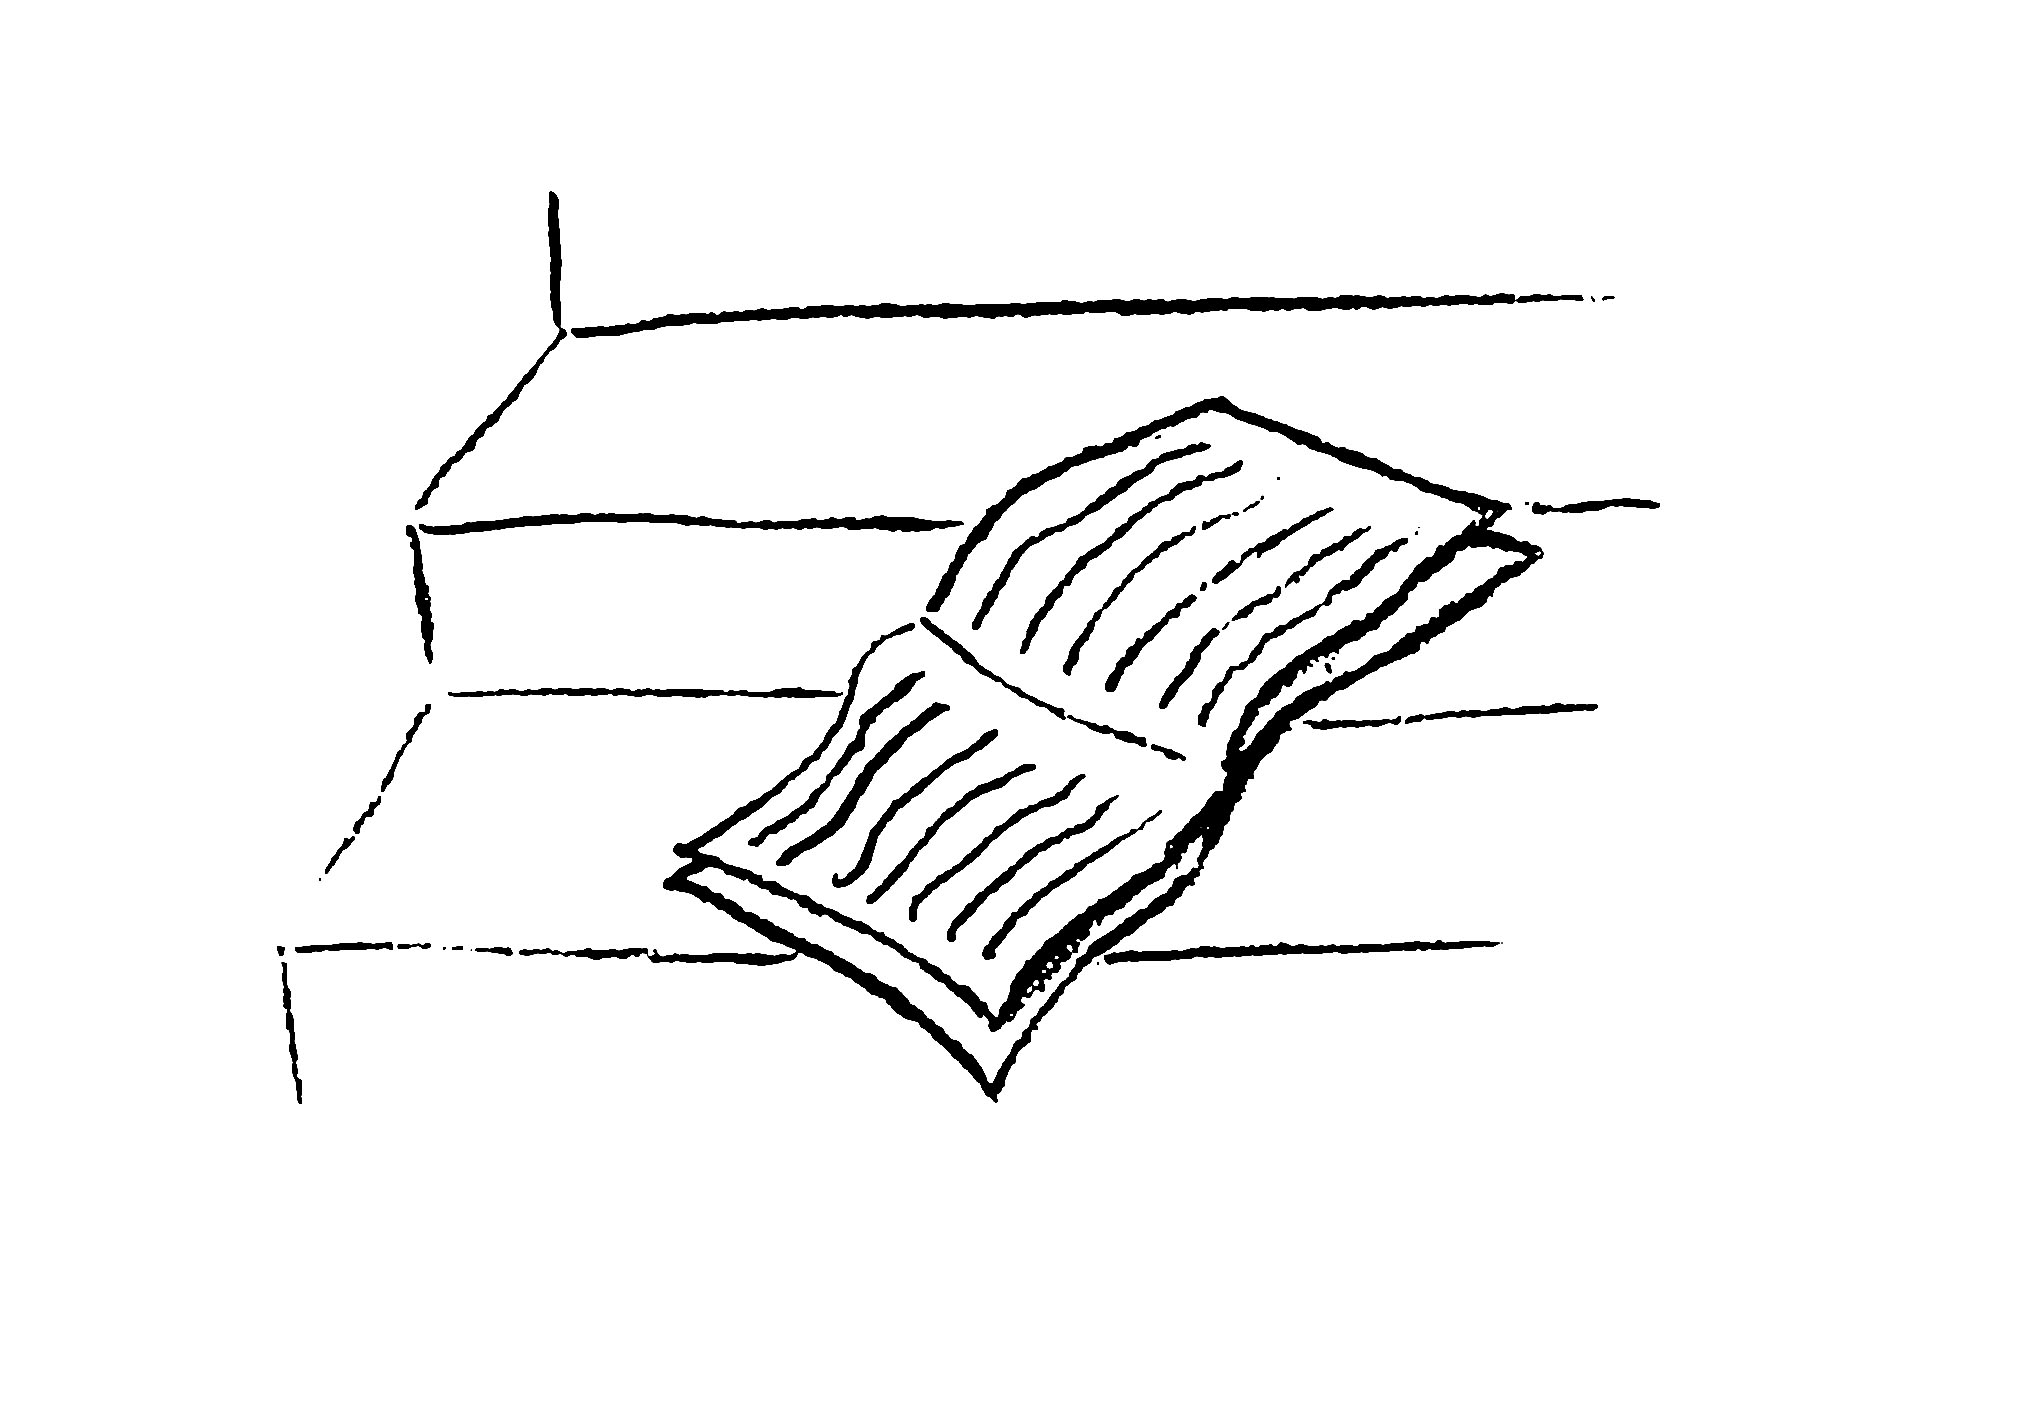
\includegraphics[width=0.95\columnwidth]{img/7.0 1 kniga.jpg}
\end{minipage}
\end{figure} 

\begin{thm}
    В блокноте 10 страниц, на каждой из них написано утверждение: 
    \par
    на первой странице: «В этом блокноте количество неверных утверждений делится на 1»;
    \par
    на второй странице: «В этом блокноте количество неверных утверждений делится на 2»;
    \par
    на третьей: «В этом блокноте количество неверных утверждений делится на 3»;
    \par
    ...
    \par
    на десятой: «В этом блокноте количество неверных утверждений делится на 10».
    \par
    Сколько в блокноте верных утверждений?
\end{thm}

\begin{thm}
    Чего больше: пятниц, кроме тех пятниц, которые не являются тринадцатыми числами, или тринадцатых чисел, кроме тех, которые не являются пятницами?
\end{thm}

\begin{thm}
    Предположим, что справедливы следующие утверждения:
    \par
    а) Среди людей, имеющих обезьянок, есть такие, которые не являются спелеологами.
    \par
    б) Люди, выращивающие кактусы, но не являющиеся спелеологами, не имеют обезьянок.
    \par
    Верно ли тогда, что не все владельцы обезьянок разводят кактусы?
\end{thm}

\begin{thm}
    Известно, что ляпусики, у которых есть варкала, не все бармаглоты. Кроме того, у тех ляпусиков, которые умеют хрюкотать и при этом не бармаглоты, варкал нет. Верно ли, что не все ляпусики, у которых есть варкала, умеют хрюкотать?
\end{thm}

\begin{thm} $^n$
    В тюрьму поместили 2011 узников. Надзиратель сказал им: «Я дам вам вечер поговорить друг с другом, а потом общаться вы не сможете. Иногда я буду одного из вас отводить в комнату, в которой есть лампа (вначале она выключена). Можно её включить или выключить. Если в какой-то момент кто-то из вас скажет мне, что вы все уже побывали в комнате, и будет прав, то я вас освобожу. А если неправ – казню. Если будете молчать, то все побываете в комнате, и ни для кого никакое посещение комнаты не станет последним». 
    \par
    Придумайте стратегию, гарантирующую узникам освобождение.
\end{thm}

\begin{figure}[H]
\begin{minipage}{0.69\linewidth}\setlength{\parindent}{1.5em}
    \begin{thm}
        Эрик увидел двух двухголовых дракончиков, головы которых спутались. Драконы бывают либо правдивые, т.е. все головы говорят только правду, либо лживые, т.е. все головы всегда лгут. Эрик решил помочь дракончикам распутать головы. Но для этого ему надо знать, где чья голова. Он спросил, какая голова чья у дракончиков, на что головы ответили: 
        \par первая голова: «я – правдивая голова»;
        \par вторая голова: «третья голова – моя родная голова»; 
        \par третья голова: «вторая голова – не родная мне голова»; 
        \par четвёртая голова: «третья голова – лживая». 
        \par Какие головы принадлежат каким дракончикам?
    \end{thm}
\end{minipage}
\hfill
\begin{minipage}{0.3\linewidth}
    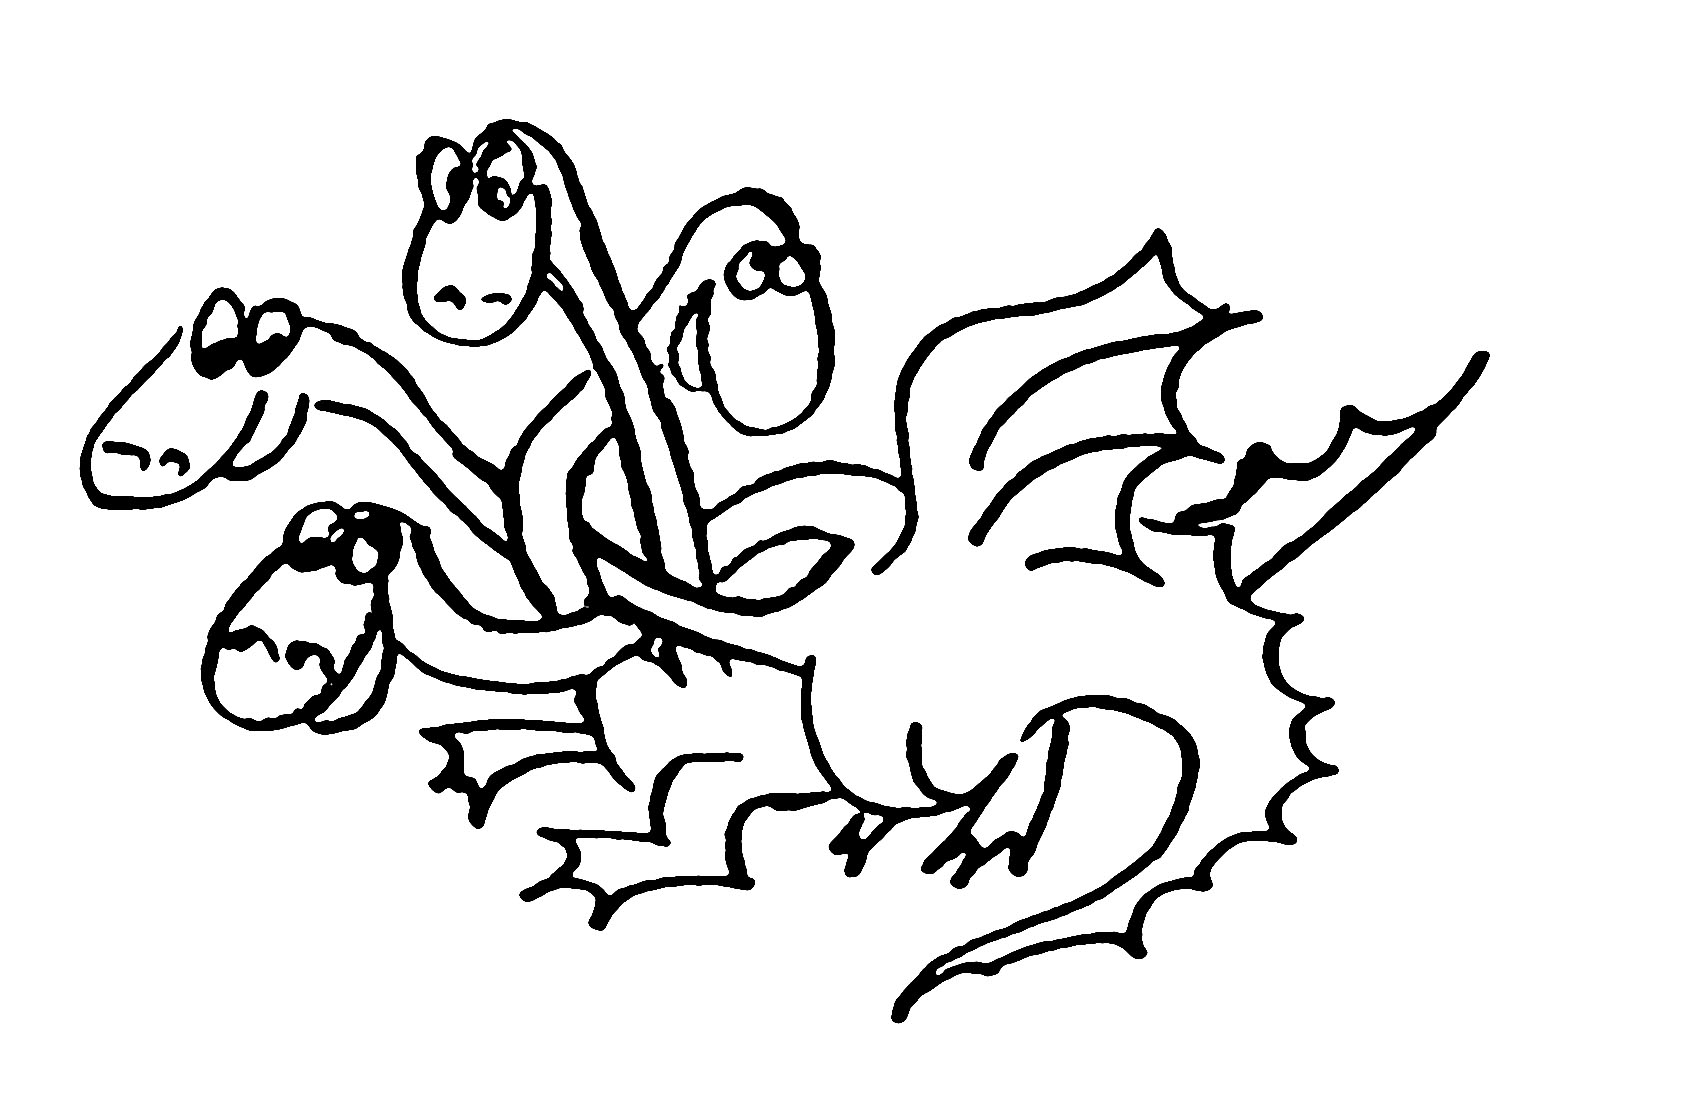
\includegraphics[width=0.95\columnwidth]{img/7.0 2 drakon.jpg}
\end{minipage}
\end{figure} 

\begin{thm} $^*$
    (по мотивам задачи Эйнштейна\footnotemark) В пяти домах с крышами разных цветов на одной стороне улицы живут пять джентльменов, каждый из которых предпочитает определённый напиток, занимается определённым видом спорта и держит животное, птицу, или разводит рыб (напитки, виды спорта и питомцы у всех разные). Известно, что:
    \par \textit{англичанин} живёт в доме с \textit{красной} крышей; 
    \par \textit{швед} держит \textit{собаку};
    \par \textit{датчанин} предпочитает \textit{чай}; 
    \par дом с \textit{зелёной} крышей расположен слева по соседству с домом под \textit{белой} крышей; 
    \par джентльмен из дома под \textit{оранжевой} крышей замечен за игрой в \textit{регби};
    \par \textit{футболист} иногда разговаривает с \textit{попугаем}; 
    \par хозяин дома с \textit{зелёной} крышей пьет \textit{кофе}, а хозяин \textit{среднего} дома – \textit{молоко};
    \par \textit{норвежец} живет в \textit{крайнем} доме, по соседству с домом с \textit{синей} крышей; 
    \par \textit{волейболист} соседствует с \textit{любителем коше}к; 
    \par \textit{любитель лошадей} живет рядом с \textit{регбистом}; 
    \par \textit{немец} играет в \textit{теннис}; 
    \par \textit{сосед волейболиста} пьет только \textit{минеральную воду}, а \textit{баскетболист} предпочитает \textit{квас}.
    \par Выясните, кто в каком доме живёт, каким видом спорта занимается, какие напитки предпочитает, а также кто разводит рыбок.
\end{thm}\footnotetext{Эйнштейн утверждал, что эту задачу не сможет решить более двух процентов мыслящего населения планеты. Интересно, к какой части относитесь вы?}

\section{Высказывания и отрицания.}

\begin{thm}
    Жители города Запузыринска ходят на руках и говорят все наоборот. Например, вместо «здравствуй» они говорят «до свидания», вместо «заходите в гости» – «катись отсюда», а вместо «вышел зайчик погулять» – «зашёл волчище посидеть». А вот какие задачи дают там на уроках математики: «Во вторую ночь заяц выплюнул 100 волков, а в первую – на 5 волков больше. Сколько волков выплюнул заяц в первую ночь?»
    \par
    а) Попробуйте перевести эту задачу на русский язык и дайте ответ.
    \par
    б) Переведите строчку из популярной запузыринской песни: “Огромной берёзе жарко летом”.
\end{thm}

\setlist{nosep} % Убирает вертикальные отступы между айтемами во всех листах


\begin{thm}
    «Все критяне – лжецы», – сказал философ с острова Крит. Какие из следующих утверждений верны, а какие нет, а о каких ничего нельзя сказать? Ответ обоснуйте.
    
    \begin{enumerate}[label=\asbuk*), ref=\asbuk*]
        \item Все критяне – лжецы.
        \item Все критяне говорят правду.
        \item Философ – лжец.
        \item Философ говорит правду.
        \item Среди критян есть лжецы.
        \item Среди критян есть говорящие правду.
    \end{enumerate}
    
\end{thm}


\begin{thm}
    Гоша \textit{верно} решил \textit{все} уравнения. Какие из перечисленных ниже утверждений являются отрицанием этого утверждения?
    
    \begin{enumerate}[label=\asbuk*), ref=\asbuk*]
        \item Петя решил верно все уравнения.
        \item Гоша решил неверно все уравнения.
        \item Гоша решил неверно одно уравнение.
        \item Гоша решил неверно какое-то уравнение.
        \item Гоша решил верно одно уравнение.
        \item Кто-то решил верно все уравнения
        \item Кто-то решил неверно все уравнения.
        \item Кто-то решил неверно какое-то уравнения.
    \end{enumerate}
    
\end{thm}


\begin{thm}
    На Уральском турнире матбоев в \textit{каждом} туре \textit{все} команды решили \textit{все} задачи. Какие из перечисленных ниже утверждений должны быть истинны\footnotemark, чтобы это утверждение стало неверным?
    
    \begin{enumerate}[label=\asbuk*), ref=\asbuk*]
        \item Была команда, которая в каждом туре не решила хотя бы одну задачу
        \item В каждом туре все команды не решили хотя бы одну задачу.
        \item Была команда, которая в каждом туре решила все задачи.
        \item Был тур, в котором ни одна из команд не решила все задачи.
        \item Была команда, которая в одном из туров решила все задачи.
        \item Во всём турнире была задача, которую не решила ни одна команда.
        \item В каждом туре все команды решили хотя бы одну задачу.
    \end{enumerate}
    
\end{thm}\footnotetext{Т.е. истинность этих утверждений является \textit{достаточной}, для того, чтобы сделать вывод.}


\begin{thm}
    На Уральском турнире матбоев \textit{не в каждом} туре \textit{все} команды решили \textit{все} задачи. Пусть это утверждение верно. Какие из перечисленных ниже утверждений обязательно должны быть истинны в этом случае?\footnotemark

    \begin{enumerate}[label=\asbuk*), ref=\asbuk*]
        \item Была команда, которая в каждом туре не решила хотя бы одну задачу
        \item В каждом туре все команды не решили хотя бы одну задачу.
        \item Была команда, которая в каждом туре решила все задачи.
        \item Был тур, в котором ни одна из команд не решила все задачи.
        \item Была команда, которая в одном из туров решила все задачи.
        \item Во всём турнире была задача, которую не решила ни одна команда.
        \item В каждом туре все команды решили хотя бы одну задачу.
    \end{enumerate}
\end{thm}\footnotetext{Т.е. истинность этих утверждений является \textit{необходимой}.}


\begin{thm}
    Назовём контрольную легкой, если за каждой партой найдется ученик, решивший все задачи. Дайте определение \textit{трудной} контрольной.
\end{thm}

\begin{thm}
    Рассмотрим два определения лёгкой контрольной: 
    \par 1) в каждом варианте каждую задачу решил хотя бы один ученик;
    \par 2) в каждом варианте хоты бы один ученик решил все задачи. 
    \par Может ли контрольная быть лёгкой в смысле определения 1) и трудной в смысле определения 2)?
\end{thm}


\section{Логические парадоксы.} 

Мы свободно говорим об истинности утверждений, высказываний... А что такое высказывание?
\par
Например, можно ли что-нибудь сказать об истинности или ложности следующих предложений:

\begin{center}
    \fbox{\begin{varwidth}{0.95\textwidth}
        Утверждение в рамке ложно
    \end{varwidth}}
\end{center}

\begin{center}
    \fbox{\begin{varwidth}{0.95\textwidth}
        \fbox{\begin{varwidth}{0.95\textwidth}
            Утверждение в двойной рамке истинно
        \end{varwidth}}
    \end{varwidth}}
\end{center}

\textit{Высказывание} – это утверждение, о котором можно сказать, истинно ли оно или ложно. Если
какое-то высказывание истинно, то его отрицание\footnote{Если рассматривать утверждения как все возможные события, то само утверждение – это множество некоторых событий, для которых это утверждение справедливо, а отрицание данного утверждения – все события, которые лежат вне этого множества.} ложно (обозначение: $A$ – само высказывание,
$\neg A$ – его отрицание). Понятно, что утверждение ''$A$ или $\neg A$ » всегда истинно (закон исключения третьего, другими словами, третьего не дано), напротив, утверждение ''$A$ и $\neg A$'' всегда ложно (закон противоречия), а двойное отрицание утверждения равносильно самому утверждению: $\neg \neg A = A$ (закон двойного отрицания).

В обычном языке можно придумать много предложений, о которых нельзя сказать, истинны они или ложны. Однако и в рамках логики существуют такие конструкции, о которых нельзя сказать, истинны они или ложны. Такие конструкции называются парадоксами. Например:

\begin{center}
    \begin{tabular}{ | m{6cm} | m{6cm} | } 
        \hline
        \textit{Утверждение справа истинно} & \textit{Утверждение слева ложно.} \\ 
        \hline
    \end{tabular}
\end{center}

\begin{figure}[H]
\begin{minipage}{0.79\linewidth}\setlength{\parindent}{1.5em}
    \begin{thm}
        \textit{(парадокс брадобрея)} Одному солдату отдали приказ брить тех и только тех, кто не бреется сам. Сможет ли он его выполнить?
    \end{thm}
    \begin{thm}
        Существует ли наименьшее целое число, которое нельзя определить при помощи фразы, состоящей не более чем из ста русских слов?
    \end{thm}
    \begin{thm}
        Как-то в 1943 году, шведское радио сообщило о том, что на следующей неделе намечено объявить воздушную учебную тревогу. Чтобы проверить готовность войск ПВО, учение решено провести внезапно так, что даже в день тревоги, ни один человек не сможет предугадать, в котором часу оно будет объявлено. Л. Экбом, преподаватель математики в Стокгольме, усмотрел в этом логический парадокс и обсудил его со своими студентами. Как вам кажется, в чём состоит этот парадокс?
    \end{thm}
\end{minipage}
\hfill
\begin{minipage}{0.2\linewidth}
    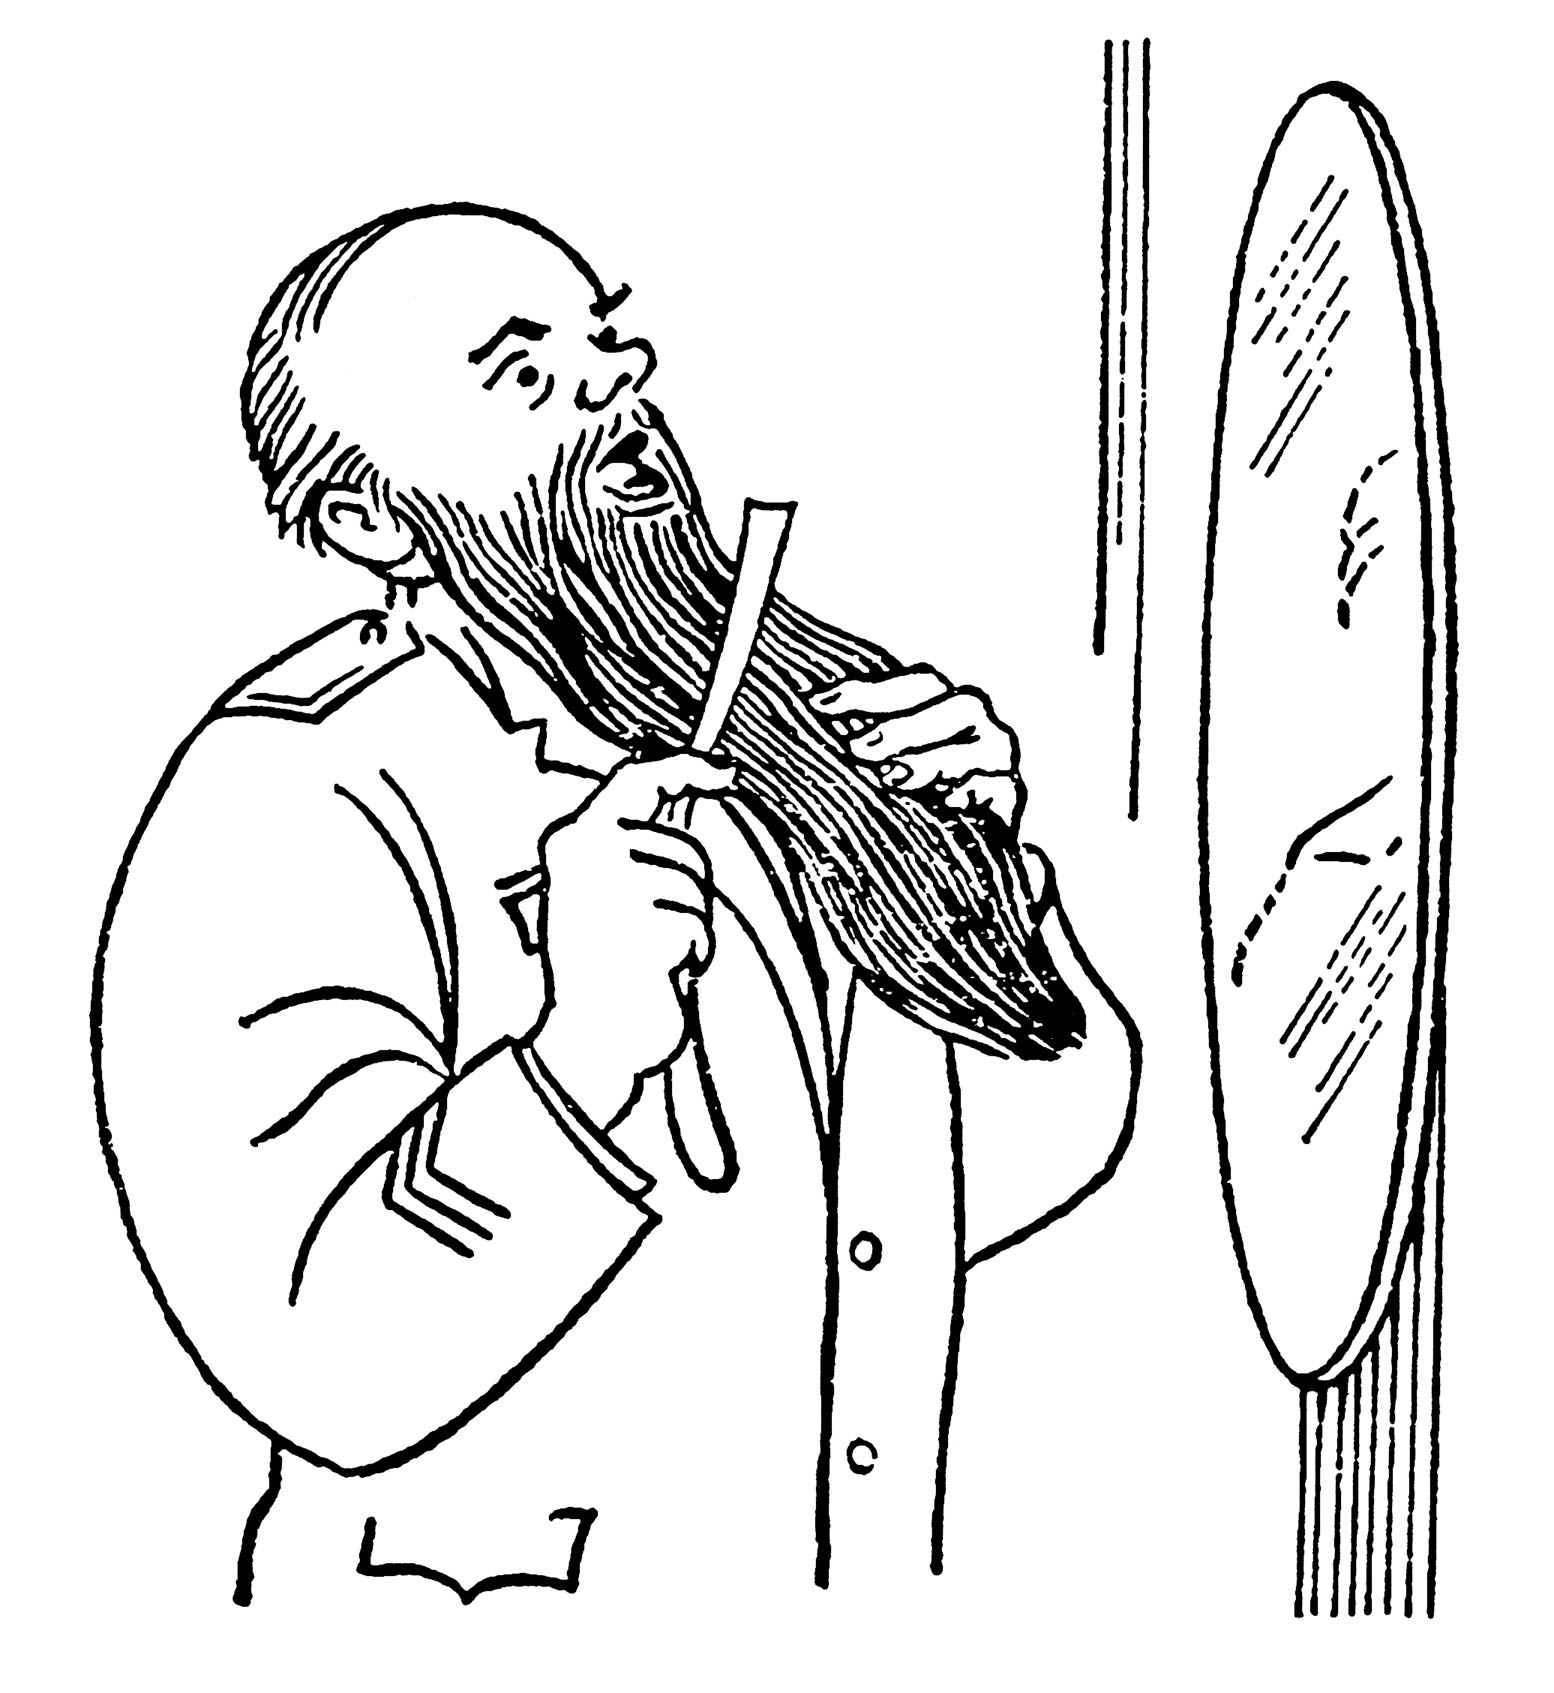
\includegraphics[width=0.95\columnwidth]{img/7.0 3 boroda.jpg}
\end{minipage}
\end{figure} 

\begin{thm}
    Племя людоедов поймало Робинзона Крузо. Вождь сказал: «Мы бы рады отпустить тебя, но по нашему закону ты сначала должен что-нибудь сказать. Если это окажется истиной – мы съедим тебя. Если же это будет ложью – тебя съест наш лев». Как спасти Робинзона?
\end{thm}

\section{Причина и следствие или «Если ... , то ... »}

\epigraph{\textit{«Если дважды два – пять, то существуют ведьмы...»}}{\textit{Феликс Хаусдорф}}

\begin{thm}
    За день до дождя Мюллер всегда чихает. Сегодня Мюллер чихнул. «Завтра будет дождь», – подумал Штирлиц. Прав ли он?
\end{thm}

\begin{figure}[H]
\begin{minipage}{0.79\linewidth}\setlength{\parindent}{1.5em}
    \begin{thm}
    Сформулируйте хотя бы одно
        \begin{enumerate}[label=\asbuk*), ref=\asbuk*]
        \item необходимое и достаточное;
        \item необходимое, но не достаточное;
        \item достаточное, но не необходимое;
        \item не необходимое и не достаточное
        \end{enumerate}
    условие того, что четырехугольник является трапецией.
    \end{thm}
\end{minipage}
\hfill
\begin{minipage}{0.2\linewidth}
    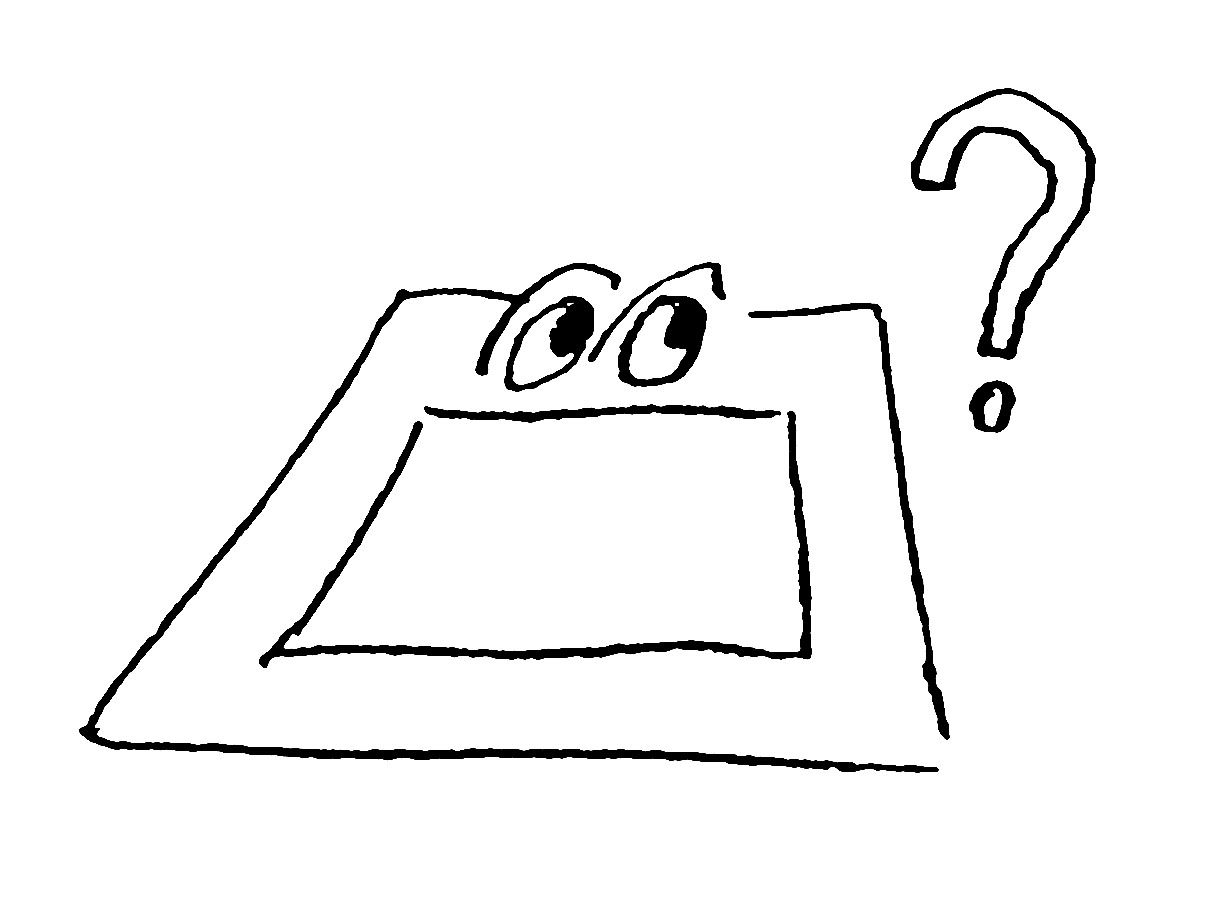
\includegraphics[width=0.95\columnwidth]{img/7.0 4 figura.jpg}
\end{minipage}
\end{figure} 

\begin{thm} \label{8.1 thm1}
    Пусть утверждение $B$: «Этот четырёхугольник – трапеция», а в качестве утверждения $A$ возьмём следующее: «У этого четырёхугольника есть две параллельные стороны». Сформулируйте 8 утверждений:
    \par
    1. Если $A$, то $B$. \hfill 2. Если $A$, то не $B$. \hfill 3. Если не $A$, то $B$. \hfill 4. Если не $A$, то не $B$.
    \par
    5. Если $B$, то $A$. \hfill 6. Если $B$, то не $A$. \hfill 7. Если не $B$, то $A$. \hfill 8. Если не $B$, то не $A$.
    \par
    Какие из этих утверждений верны, а какие нет?
\end{thm}

\begin{thm} \label{8.1 thm3}
    Пусть теперь $A$ и $B$ – какие-то утверждения (каждое из них либо истинно, либо ложно). Рассмотрим восемь теорем:
    \par
    1. Если $A$, то $B$. \hfill 2. Если $\overline{A}$, то $B$. \hfill 3. Если $A$, то $\overline{B}$. \hfill 4. Если $\overline{A}$, то $\overline{B}$.
    \par
    5. Если $B$, то $A$. \hfill 6. Если $\overline{B}$, то $A$. \hfill 7. Если $B$, то $\overline{A}$. \hfill 8. Если $\overline{B}$, то $\overline{A}$.
    \par
    Известно, что теорема 1 верна. Разбейте оставшиеся семь теорем на три группы: те, которые заведомо верны, те, которые заведомо неверны и те, о которых ничего определённо сказать нельзя (т.е. они могут быть верными или неверными в зависимости от выбора утверждений $A$ и $B$).\footnotemark
\end{thm}\footnotetext{Договоримся не рассматривать в качестве $A$ и $B$ утверждения, которые всегда истинны или всегда ложны, например, ''В квадрате все углы тупые'' или ''На плоскости прямые параллельны или пересекаются''.}

Заметим, что предыдущую задачу можно интерпретировать на языке множеств. Т.к. в высказывании речь идёт о некоторых объектах, то по отношению, скажем, к высказыванию $A$ все эти объекты можно разбить на два множества: множество объектов, для которых высказывание верно и множество, для которых неверно. Так сказать, $A$ и $\overline{A}$. (Например, утверждение $A$: «Данный четырёхугольник – параллелограмм», утверждение $B$: «данный четырёхугольник имеет равные стороны».) Тогда что на языке множеств означает наша теорема 1? Только то, что если объект принадлежит множеству $A$, то он принадлежит и множеству $B$!

\begin{thm} $^*$
    Какой смысл по-вашему мнению имеет высказывание Феликса Хаусдорфа, вынесенное в эпиграф?
\end{thm}

\begin{thm} \label{8.1 thm2}
    Однажды утром метеостанция маленького города Новозыбкова передала необычный прогноз погоды. Этот прогноз состоял из нескольких утверждений:
    \begin{enumerate}
        \item Если сегодня дождя не будет, то завтра будет ветреная погода.
        \item Если сегодня пойдёт дождь, то завтра без осадков.
        \item Если сегодня будет холодно, то влажность воздуха сегодня будет высокой.
        \item Если сегодня будет тепло, то завтра безветренно.
        \item Если сегодня ветра нет, то завтра будет тепло при высокой влажности и дождь.
        \item Если сегодня ветреная погода, то завтра – низкая влажность воздуха, но будет дождь.
        \item Если сегодня влажность будет высокой, то завтра она останется без изменений.  
    \end{enumerate}
    Допустим, что каждое утверждение синоптиков верно. Определите в этом случае погоду (т.е. температуру, осадки, влажность и ветер) на сегодня и завтра.
\end{thm}


\begin{center}
    \textit{\textbf{Лирическое отступление.}}
\end{center}

В курсе геометрии вы доказывали следующие утверждения: «Если четырёхугольник – параллелограмм, то его стороны попарно равны.», «Если четырёхугольник – параллелограмм, то его диагонали делятся точкой пересечения пополам.» Отсюда справедливо утверждение: «Если четырёхугольник – параллелограмм, то его стороны попарно равны и диагонали делятся точкой пересечения пополам».
Рассмотрим ещё один пример. В школьной столовой сок стоит 3 руб., а булочка – 2 руб. Справедливы следующие утверждения: «Если у Полины есть 3 рубля, то она может купить булочку.», «Если у Полины
есть 3 рубля, то она может купить сок.» Отсюда справедливо утверждение: «Если у Полины есть 3 рубля, то
она может купить булочку и сок.» ... Рассуждения аналогичны. В чём тут дело?

\section{«Сложносочинённые» утверждения.}

Пусть имеется набор некоторых высказываний, про которые можно узнать, истинны они или ложны. Будем обозначать их заглавными буквами: $A$, $B$, $C$ и т.д. Как и в обычном языке, из уже имеющихся высказываний можно, как из кирпичиков, строить новые. Например, в задачах \ref{8.1 thm1} – \ref{8.1 thm2} высказывания были построены с помощью конструкции «если $A$, то $B$»\footnote{В этом случае высказывание $A$ называется посылкой, а высказывание $B$ – следствием или заключением}. Как из простых предложений можно строить сложносочинённые предложения, где все входящие предложения равноправны, так и из «простых» высказываний можно строить сложные с помощью союзов «и» и «или».

\begin{dfn}
    Пусть $A$ и $B$ – некоторые высказывания. Тогда $A \vee B$ – \textit{дизъюнкция (логическое сложение)} высказываний $A$ и $B$. (Читается «$A$ или $B$» ) Это высказывание истинно, когда хотя бы одно из входящих в него простых высказываний истинно, а ложно, когда ложны все высказывания.
\end{dfn}

\begin{dfn}
    Аналогично, $А \& \ В$\footnote{Также используется обозначение $A \wedge B$.} – \textit{конъюнкция (логическое умножение)} высказываний $A$ и $B$. (Читается «$A$ и $B$» ) Это высказывание истинно только когда истинны все входящие в него высказывания, а ложно, когда ложно хотя бы одно.
\end{dfn}

Для наглядности запишем в табличку:

\begin{figure}[H]
\begin{minipage}{0.45\linewidth}\setlength{\parindent}{1.5em}
    \begin{center}
        \begin{tabular}{ |c|c|c| } 
            \hline
             $A$ & $B$ & $A \vee B$ \\ 
             \hline
             \textit{истина} & \textit{истина} & \textit{истина} \\ 
             \hline
             \textit{истина} & \textit{ложь} & \textit{истина} \\ 
             \hline 
             \textit{ложь} & \textit{истина} & \textit{истина} \\ 
             \hline 
             \textit{ложь} & \textit{ложь} & \textit{ложь} \\ 
             \hline
        \end{tabular}
    \end{center}
\end{minipage}
\hfill
\begin{minipage}{0.45\linewidth}
    \begin{center}
        \begin{tabular}{ |c|c|c| } 
            \hline
             $A$ & $B$ & $A\  \& \ B$ \\ 
             \hline
             \textit{истина} & \textit{истина} & \textit{истина} \\ 
             \hline
             \textit{истина} & \textit{ложь} & \textit{ложь} \\ 
             \hline 
             \textit{ложь} & \textit{истина} & \textit{ложь} \\ 
             \hline 
             \textit{ложь} & \textit{ложь} & \textit{ложь} \\ 
             \hline
        \end{tabular}
    \end{center}
\end{minipage}
\end{figure} 

Почему эти операции называют сложением и умножением станет понятнее, если считать значение «истина» равным 1, а значение «ложь» – 0.\footnote{Правда, при сложении нам придется договориться, что 1 + 1 = 1.}

\begin{ex}
    Решите примеры:
    \par
    \textbf{1}. 1 $\vee$ 0 = ? \hfill 
    \textbf{2}. 0 $\&$ 1 = ? \hfill
    \textbf{3}. 1 $\&$ (0 $\vee$ 1) = ? \hfill
    \textbf{4}. (1 $\&$ 1) $\vee$ (0 $\vee$ 1) = ? \hfill
    \textbf{5}. 0 $\vee$ (0 $\vee$ (0 $\vee$ 1)) = ?
\end{ex}

\begin{ex}
    Вычислите значение выражения, если $A$ истинно, а $B$ - ложно:
    \par
    \textbf{1}. $B$ $\vee$ $A$ \hfill 
    \textbf{2}. $A$ $\&$ $\overline{B}$ \hfill
    \textbf{3}. $A$ $\&$ ($\overline{A}$ $\vee$ $\overline{B}$) = ? \hfill
    \textbf{4}. ($\overline{A}$ $\&$ $\overline{B}$) $\vee$ ($\overline{A}$ $\vee$ $B$) \hfill
    \textbf{5}. $\overline{A}$ $\vee$ ($\overline{B}$ $\vee$ ($B$ $\vee$ $A$))
\end{ex}

\begin{thm}
    Антон лжёт по понедельникам, вторникам и средам, а в остальные дни говорит только правду. Выясните, в какие дни недели Антон может заявить:
    \par а) Я лгал вчера и буду лгать завтра.
    \par б) Я лгал вчера или буду лгать завтра. 
    \par в) Я не лгал вчера и не буду лгать завтра.
    \par г) Я не лгал вчера или не буду лгать завтра.
\end{thm}

\begin{thm}
    Известно, что утверждение «$A$ или не $B$» истинно. Что вы можете сказать про истинность утверждений $A$ и $B$. А если утверждение «$A$ или не $B$» ложно?
\end{thm}

\begin{thm}
    На улице \textit{светит солнце} и у Оли \textit{плохое} настроение. Какие из перечисленных ниже утверждений являются отрицанием этого утверждения?
    \begin{enumerate}[label=\asbuk*), ref=\asbuk*]
        \item На улице пасмурно и у Оли хорошее настроение.
        \item На улице пасмурно или у Оли хорошее настроение.
        \item На улице пасмурно и у Оли плохое настроение.
        \item На улице пасмурно или у Оли плохое настроение.
        \item На улице светит солнце и у Оли хорошее настроение.
        \item На улице светит солнце или у Оли хорошее настроение.
    \end{enumerate}
\end{thm}

\begin{thm}
    На уроке алгебры Андрей получил \textit{пятёрку или четвёрку}. Какие из перечисленных ниже утверждений являются отрицанием этого утверждения?
    \begin{enumerate}[label=\asbuk*), ref=\asbuk*]
        \item На уроке алгебры Андрей получил пятёрку и четвёрку.
        \item На уроке алгебры Андрей получил двойку и тройку.
        \item На уроке алгебры Андрей получил двойку или тройку.
        \item На уроке алгебры Андрей не получил пятёрку и не получил четвёрку.
        \item На уроке алгебры Андрей не получил пятёрку или не получил четвёрку.
        \item На уроке алгебры Андрей получил пятёрку, но не получил четвёрку.
        \item На уроке алгебры Андрей не получил пятёрку, но получил четвёрку.
    \end{enumerate}
\end{thm}

\begin{dfn}
    Пусть $А$ и $В$ – некоторые высказывания. Конструкция «если ... , то ... » называется \textit{логическим следованием} или \textit{импликацией}. Обозначение $А \Rightarrow В$.
\end{dfn}

\begin{ex}
    Составьте табличку значений для импликации и сравните полученные результаты с результатом задачи \ref{8.1 thm3}.
\end{ex}
\head{Сентябрь}{Листок 8. Логика. Уровень 0.}

\epigraph{\textit{– Разве это ложь? – сказала Королева. – Слыхала я такую
ложь, рядом с которой эта правдива, как толковый словарь!}}{\textit{Л. Кэрролл "Алиса в Зазеркалье"}}

Безусловно, вы уже сталкивались с задачами, в которых нужно рассматривать случай, когда кто-то лжёт. Соответственно встаёт вопрос об истинности или ложности некоторых утверждений. Позже мы разберём это подробнее, а пока то, что есть «правда», а что «ложь», мы будем считать интуитивно понятным. Для начала несколько простых упражнений.
\\
Напомним, что «рыцари» всегда говорят правду, а «лжецы» всегда лгут.

\begin{ex}
    Известно, что в ящике лежит 17 шариков. Какие из приведенных ниже утверждений являются всегда истинными, а какие – всегда ложными
    \begin{enumerate}[label=\asbuk*), ref=\asbuk*]
        \item В ящике не менее 17 шариков.
        \item В ящике лежит 17 шариков или 15 шариков.
        \item В ящике найдётся 15 шариков.
        \item В ящике есть шарики разных цветов.
        \item В ящике найдётся не более 17 одноцветных шариков.
        \item В ящике не менее двух шариков одного размера.
        \item Из ящика нельзя вытащить 20 шариков одного цвета.
        \item Шарики в ящике можно сложить по парам.
    \end{enumerate}
\end{ex}

\begin{ex}
    После победы над Змеем Горынычем три богатыря заявили:
    \par
    \underline{Илья Муромец}: «Змея убил Добрыня Никитич».
    \par
    \underline{Добрыня Никитич}: «Змея убил Алёша Попович».
    \par
    \underline{Алёша Попович}: «Змея убил я».
    \par
    Кто убил Змея и почему именно он, если только один из них сказал правду?
\end{ex}

\begin{ex}
    В комнате находятся рыцарь и лжец. Кто из них мог сказать фразу: «Мы оба лжецы»?
\end{ex}

\begin{ex}
    На острове рыцарей и лжецов житель $A$ в присутствии другого жителя $B$ говорит: «По крайней мере один из нас – лжец». Кто такие $A$ и $B$?
\end{ex}

\begin{ex}
    В комнате 2012 жителей острова рыцарей и лжецов. Каждый из них заявил: «Кроме меня в комнате все лжецы!». Сколько рыцарей в комнате?
\end{ex}

\begin{ex}
    В комнате 2012 жителей острова рыцарей и лжецов. Одного из них зовут Ваня. Они встали в круг, и Миша – правый сосед Вани – сказал: «Ваня, ты лжец!». Тогда правый сосед Миши сказал: «Ты не прав!», и так далее: каждый (кроме Вани) по кругу высказал своему соседу, что он неправ. Сколько в комнате лжецов?
\end{ex}

\begin{ex}
    А если в предыдущей задаче каждый (кроме Вани) сказал «Ты прав!», то сколько тогда было бы в комнате лжецов?
\end{ex}

\begin{ex}
    У Снусмумрика украли флейту. Известно, что те, кто крадут флейты, всегда лгут. «Я знаю, кто украл флейту!», – заявил Мумми-тролль. Виновен ли Мумми-тролль?
\end{ex}

\begin{ex}
    Среди трёх человек $A$, $B$ и $C$ один лжец, один рыцарь, а третий – нормальный человек, который может говорить и правду, и ложь. 
    $A$ говорит: «Я нормальный человек».
    $B$ говорит: «$A$ и $C$ иногда говорят правду». 
    $C$ говорит: «$B$ – нормальный человек».
    Кто из них кто?
\end{ex}

\begin{ex}
     В конференции участвовало 100 человек – химиков и алхимиков. Каждому был задан вопрос: «Если не считать Вас, то кого больше среди остальных участников – химиков или алхимиков?». Когда опросили 51 участника, и все ответили, что алхимиков больше, опрос прервался. Алхимики всегда лгут, а химики говорят правду. Сколько химиков среди участников?
\end{ex}

\begin{ex}
    В комнате четыре человека – жители острова рыцарей и лжецов каждый из них сделал заявление.
    \par
    Первый: «среди нас не более одного лжеца».
    \par
    Второй: «среди нас не более двух лжецов».
    \par
    Третий: «среди нас не более трех лжецов».
    \par
    Четвёртый: «среди нас не более четырех лжецов».
    \\
    Сколько рыцарей в комнате?
\end{ex}

\begin{ex}
    У Карабаса-Барабаса украли пять золотых. Карабас подозревает в краже лису Алису, кота Базилио, Дуремара и Буратино, так как неопровержимыми уликами установлено, что 
    \par
    кто-то из них обязательно виновен; 
    \par
    никто больше не мог это сделать;
    \par
    Алиса всегда действует заодно с Базилио;
    \par
    если Дуремар виновен, то у него было ровно 2 соучастника;
    \par
    если Буратино виновен, то у него был ровно 1 соучастник.
    \\
    Нужно определить, виновен ли Базилио.
\end{ex}

\section{Наконец-то, задачи!}

В следующих задачах не требуется ничего, кроме здравых рассуждений. Напоминаем, что задачи, отмеченные значком \textit{п}, являются письменными, и в устном виде приниматься не будут. Отмеченные звёздочками не являются обязательными (это не значит, что они сложнее).

\begin{thm} $^n$
    Мама пришла с работы домой и обнаружила, что коробка с конфетами пуста. На вопрос «Кто съел конфеты?» её дочери Вета, Рая и Соня ответили так:
    \par
    Вета: «Соня не ела последнюю конфету» 
    \par
    Рая: «Соня и Вета обе ели конфеты»
    \par 
    Соня: «Рая и Вета обе не ели конфеты».
    \\ 
    Впоследствии оказалось, что все сказали неправду. Кто съел конфеты?
\end{thm}

\begin{thm}
    На острове невезения живут 2012 человек. Некоторые из них всегда лгут, а остальные всегда говорят правду. Каждому жителю острова не везёт только в один из трёх дней: понедельник, среду или пятницу. Однажды каждому жителю острова задали три вопроса:
    \par
    1. «Вам не везёт в понедельник?»
    \par 
    2. «Вам не везёт в среду?»
    \par
    3. «Вам не везёт в пятницу?»
    \\
    На первый вопрос ответили «да» 999 человек, на второй – 1000, на третий – 1001. Сколько лжецов на острове?
\end{thm}

\begin{thm}
    В комнате сидело 2012 жителей острова рыцарей и лжецов. В какой-то момент один человек обиделся и ушёл. Один из оставшихся, поглядев в след, заметил: «Ушедший – лжец!» После чего встал и тоже вышел. Второй сказал: «Оба ушедшие – лжецы» и тоже ушёл. Далее каждый из оставшихся уходил, говоря: «Все ушедшие – лжецы». Пока последний оставшийся в комнате печально не констатировал: «Да, все ушедшие – лжецы».
    \\
    Определите, сколько в комнате было лжецов первоначально. (Лжецы всегда лгут, рыцари всегда говорят правду)
\end{thm}

\begin{thm}
    На планете «Куб» (имеющей форму куба) каждой гранью владеет рыцарь или лжец. Каждый из них утверждает, что среди его соседей лжецов больше, чем рыцарей. Сколько рыцарей и сколько лжецов владеют гранями планеты?
\end{thm}

\begin{thm}
    Однажды каждый житель планеты «Куб» из предыдущей задачи (возможно, теперь они владеют гранями планеты как--то по--другому) сделал заявление: «Среди моих соседей лжецов больше, чем рыцарей». Можно ли поменять местами двух человек, чтобы каждый из них мог сказать «Среди моих соседей рыцарей больше, чем лжецов»?
\end{thm}

\newpage

\begin{thm}
    Министры иностранных дел Ассирии, Аримака и Такито обсудили за закрытыми дверями проекты соглашения о полном разоружении, представленные каждой из стран. Отвечая затем на вопрос журналистов: «Чей именно проект был принят?», министры дали такие ответы:
    \par
    Ассирия: «Проект не наш. Проект не Аримаки»;
    \par
    Аримака: «Проект не Ассирии. Проект Такито»;
    \par
    Такито: «Проект не наш. Проект Ассирии».
    \\
    Один из них (самый откровенный) оба раза говорил правду; второй (самый скрытный) оба раза говорил неправду, третий (осторожный) один раз сказал правду, а другой раз – неправду. Определите, чей проект был принят.
\end{thm}

\begin{thm}
    а) Обязательно ли является ли старейший шахматист среди музыкантов старейшим музыкантом среди шахматистов?
    \par
    б) Обязательно ли является ли лучший шахматист среди музыкантов лучшим музыкантом среди шахматистов?\footnotemark
\end{thm}\footnotetext{Подумайте сначала, чем отличается шахматист среди музыкантов от музыканта среди шахматистов.}
\head{Сентябрь}{Листок 8. Логика. Уровень 1.}

% Уровень 1

\begin{thm}
    Школьники Иванов, Петров и Никитин сидели на скамейке. Их звали Ваня, Петя и Никита. Неожиданно Никитин сказал Пете: «А ты знаешь, что среди нас нет человека, у которого фамилия образована от его имени?» Назовите полные имена мальчиков. Под полным именем мальчика будем подразумевать его имя и фамилию.
\end{thm}

\begin{thm}
    Вася, Коля, Илья и Женя живут в разных городах: Москве, Киеве, Париже и Берлине. Известно, что если Женя живёт в Москве, то Илья не парижанин. Если же Илья – москвич, то Вася живёт не в Париже. Кроме того, известно, что Вася никогда не был в Москве и Киеве, а Коля – в Берлине и Париже. Илье не довелось побывать в Киеве и Берлине. А Женя мечтает съездить в Париж. В каких городах живёт каждый из мальчиков?
\end{thm}

\begin{thm}
    Костя, Женя и Миша имеют фамилии: Орлов, Соколов и Ястребов. Какую фамилию имеет каждый мальчик, если Женя, Миша и Соколов – члены математического кружка, а Миша и Ястребов занимаются музыкой?
\end{thm}

\begin{thm}
    3 мальчика, приехавшие в выездную школу из разных городов, рассказывают о себе:
    \par
    Петя: «Я живу в Москве, а Миша в Волгограде».
    \par
    Миша: «Я живу в Москве, а Петя в Архангельске».
    \par
    Коля: «Я живу в Москве, а Петя в Волгограде».
    \\
    Их учитель, удивлённый противоречиями в сказанном, попросил их объяснить, где правда, а где ложь. Тогда ребята признались, что в сказанном каждым из них одно утверждение – правда, а второе – ложно. В каком городе живёт каждый из мальчиков?
\end{thm}

\begin{thm} $^n$
    Ниф-Ниф, Наф-Наф и Нуф-Нуф пришли в казино в серебряной, золотой и платиновой цепях. Перстни у них были из тех же металлов. У Ниф-Нифа цепь и перстень были изготовлены из одинакового металла. У Наф-Нафа ни цепь, ни перстень не были серебряными. У Нуф-Нуфа цепь была из платины, а перстень не из платины. У кого из чего были изготовлены украшения?
\end{thm}

\begin{thm}
    Три друга – Пётр, Роман и Сергей – учатся на математическом, физическом и химическом факультетах. Если Пётр – математик, то Сергей не физик. Если Роман не физик, то Пётр - математик. Если Сергей не математик, то Роман – химик. Сможете ли Вы определить специальность каждого?
\end{thm}

\begin{thm}
    Дима, Катя, Миша, Света и Юра проводили лето на даче вместе с родителями. Все дети разного возраста: от 4-x до 8-ми лет. У каждого из них своя любимая еда (бананы, мороженое, пиццa, спагетти, шоколад). И каждый чего-нибудь боится (грозы, пауков, привидений, собак, темноты). Определите сколько лет каждому из них, у кого какая любимая еда, и кто чего боится.

    \begin{enumerate}
        \item Девочки старше остальных, ни одна из них не боится темноты, и обе не любят шоколад.
        \item Света обожает пиццу и не страшится пауков
        \item Пятилетний ребёнок больше всего боится привидений.
        \item Шестилетний ребёнок боится грозы и равнодушен к шоколаду и спагетти.
        \item Самый младший ребёнок любит есть бананы, а самый старший не боится собак.
        \item Ни Дима (ему не пять лет), ни Миша не боятся ни темноты, ни пауков, и оба не любят бананы.
    \end{enumerate}
    \textit{\textbf{Замечание.}} Считается, что возраст выражается целым числом лет без учёта месяцев.
\end{thm}

\begin{thm}
    Четыре подруги пришли на каток, каждая со своим братом. Они разбились на пары и начали кататься. Оказалось, что в каждой паре «кавалер» выше «дамы», и никто не катается со своей сестрой. Самым высоким в компании был Паша Воробьев, следующим по росту – Юра Егоров, потом – Люся Егорова, Серёжа Петров, Оля Петрова, Дима Крымов, Инна Крымова и Аня Воробьева. Кто с кем катался?
\end{thm}

\newpage

\begin{thm}
    В одном из институтов учатся 4 друга. Самый младший учится на 1 курсе, а старший – на 4. Известно, что Борис – персональный стипендиат, Василий летом должен ехать на практику в Омск, а Иванов – домой в Донбасс. Николай курсом старше Петра, Борис и Орлов – коренные ленинградцы, Крылов в прошлом учебном году окончил школу и поступил на факультет, где учится Карпов. Борис иногда пользуется прошлогодними конспектами Василия. Надо определить имя и фамилию каждого из друзей и курс, на котором он учится.
    \\
    \textit{\textbf{Замечание.}} Чтобы получить персональную стипендию нужно отучиться в институте не менее года.
\end{thm}

% Некоторые задачи вырезаны из-за того, что они уже есть в Оверлифе, в файле 8.0

% Уровень 1а

\begin{thm}
    Однажды в летнем лагере за круглым столом собрались пять ребят родом из Москвы, Астрахани, Новгорода, Перми, Костромы. Их звали: Юра, Толя, Лёша, Коля, Витя. Москвич сидел между Витей и жителем Костромы, астраханец – между Юрой и Толей, а напротив его сидели пермяк и Лёша. Коля никогда до этого не был в Астрахани, Юра не был в Москве и Костроме, а костромич с Толей регулярно переписываются. Определите, в каком городе живёт каждый из ребят.
\end{thm}

\begin{thm}
    За столиком в кафе собрались трое друзей: Белокуров, Рыжов и Чернов. Брюнет сказал Белокурову: «Любопытно, что один из нас блондин, другой брюнет, а третий рыжий, но ни у кого цвет волос не совпадает с фамилией». Какой цвет волос у каждого из них?
\end{thm}

% Файл "Уровень 2" состоит из второй половины Оверлифного файла 8.0. Как итог я добавил единственную не дублированную задачу из 2 Уровня сюда.

\begin{center}
    \textbf{«Перевёртыши»}
\end{center}
В выездных школах достаточно популярна игра в перевёртыши – когда известная фраза зашифровывается путём замены каждого из слов на условно противоположное. Например: По морю ёлка плыла (Во поле берёза стояла). Вам предлагается расшифровать приведённые ниже перевёртыши.
\begin{enumerate}
    \item Быстро сутки тонут близко. 
    \item Год помирай, год тупи.
    \item Некоторые жертвы могут догадаться, откуда прыгают ёжики.
    \item От одной лисы побежишь – всех разгонишь. 
    \item Десять на машине, включая кошку.
    \item Вы читали, вы читали, ваши ноженьки взбодрились.
    \item Птичка в небе полетала и сто баксов потеряла. Села птичка на забор – продавала всем топор.
    \item Один, один, один зелёный папоротник. 
    \item Три начала, три квадрата, и в конце гайка.
    \item Стоит Скиф около моря. Слышит Скиф – на море лебедь.
    \item Сиди тут – известно где, убери это – известно кого.
    \item Ежедневно знойным мигом ты в долину убегаешь.
    \item Стоит лягушка замирает, смеётся в остановке.
    \item Сдохли у ребёнка три занудных львёнка.
    \item Жара без мглы – поганый вечер.
    \item Подобрали зайку с крыши, прикрепили зайке крылья.
    \item У лисы какой-то чёрт отнял буханку хлеба.
\end{enumerate}
\head{Сентябрь}{Листок 8. Логика. Математический бой.}

\begin{enumerate}

    \item 
    Каждый житель острова Невезения — либо рыцарь, который всегда говорит правду, либо лжец, который всегда лжёт, причём лжецов на острове ровно 33. Однажды каждый житель острова заявил: «Среди всех жителей острова, не считая меня, не меньше трети лжецов». Сколько жителей может быть на острове? Перечислите все возможности и докажите, что других возможностей нет.
    
    \item 
    На собрании лжецов и рыцарей путешественник пытается определить самого старшего. Ему известно, что среди присутствующих лжецов и рыцарей поровну, а также, что возрасты всех различны. Ему разрешается выбрать любую группу людей и спросить любого из присутствующих, кто в этой группе самый старший. Докажите, что путешественник не сможет гарантированно определить самого старшего, сколько бы вопросов он ни задавал.
    
    \item 
    Рыцари и лжецы встали в хоровод, при этом некоторые из них знакомы, а некоторые -- нет. Каждый сказал своему левому соседу: «Я знаю, кто ты, и я знаю, что ты лжец». Докажите, что лжецов в круге не меньше половины.
    
    \item 
    Каждый островитянин произнёс две фразы: «Среди моих знакомых островитян более двух лжецов» и «Среди моих знакомых островитян более трёх рыцарей». Докажите, что лжецов на острове не меньше, чем рыцарей

    \item 
    На острове Невезения ровно 1 житель сказал: «Есть лжец выше меня», 
    \\ ровно 2 жителя сказали: «Есть хотя бы двое лжецов выше меня», 
    \\ ... , 
    \\ ровно 20 жителей сказали: «Есть хотя бы 20 лжецов выше меня». 
    \par Известно, что все островитяне — разного роста, и каждый житель высказался ровно один раз. Сколько лжецов живёт на острове? Напомним, что рыцари всегда говорят правду, а лжецы всегда лгут.

    \item 
    Среди 300 человек есть 100 Петь, 100 Гош и 100 Мить. После того, как каждому задали вопрос, как его зовут, получилось 100 ответов «Петя», 100 ответов «Гоша» и 100 ответов «Митя». Известно, что ровно 80 Петь и ровно половина Гош всегда лгут, а остальные Пети и Гоши всегда говорят правду. Какое наибольшее число Мить могут быть кристально честными?

    \item 
    На острове живут рыцари, которые всегда говорят правду и лжецы, которые всегда лгут. Встретились три островитянина: Михаил Михайлович, Сергей Сергеевич, и Анатолий Анатольевич. Михаил сказал: «Мы все лжецы». Сергей на это ему ответил: «Нет, только ты». Кто есть Анатолий  — рыцарь, или лжец?

    \item 
    На острове появилось новое сообщество -- хитрецы, которые иногда говорят правду, а иногда лгут. За круглым столом сидят представители рыцарей, лжецов, и хитрецов. Каждый из сидящих произнёс две фразы:
    \par 1) «Слева от меня сидит лжец.» 
    \par 2) «Справа от меня сидит хитрец.»
    \\ Докажите, что за этим столом рыцарей сидит столько же, сколько и лжецов.
    
    \item 
    Дорогу разделили на 2011 частей (не обязательно одинаковой длины). Яна знает длину дороги. Ей разрешено спросить, чему равно расстояние между серединами любых двух частей, при этом количество вопросов не ограничено. Длину каких частей она сможет узнать?

    \item 
    \textit{Лесногородская головоломка}. 
    \par Все жители санатория «Лесной Городок» делятся на 4 типа:
    \\ 1) Титаны в здравом уме; 
    \\ 2) Титаны, лишившиеся рассудка;
    \\ 3) Друиды, находящиеся в здравом уме
    \\ 4) Друиды, лишённые рассудка. 
    \\ Титаны в здравом уме всегда говорят истину (их утверждения правильны и сами титаны честны). Титаны, лишённые рассудка, всегда лгут (в силу собственных заблуждений, но не умышленно!). Друиды в здравом уме тоже всегда лгут (в силу своей природы, а не по заблуждению). 
    \\ Друиды, лишённые рассудка, всегда говорят правду (они убеждены в своих ложных утверждениях, но при этом умышленно лгут).
    \\ Однажды три Титана делились впечатлениями о прогулках по санаторию, совершенными в разное время. Первый Титан сказал:
    \\ -- Я встретил одного человека по имени Лёша и спросил его, является ли он Титаном в здравом уме. Он мне ответил вполне определённо («да» или «нет»), но я так и не понял, к какому типу он принадлежит.
    \\ -- Я тоже встретил этого Лёшу, -- сказал второй Титан. -- Я спросил у него, является ли он Друидом, лишившимся рассудка, и он ответил определённо («да» или «нет»), однако я не понял, кем он был в действительности.
    \\ -- Я тоже встретил этого Лёшу! -- воскликнул третий Титан. -- Я спросил у него, является ли он Друидом в здравом уме, и он также ответил определённо («да» или «нет»), однако я всё равно не понял, кто он!
    \\ Кто же такой -- Лёша?
\end{enumerate}
\head{Сентябрь}{Листок 8. Логика. Уровень 1. Проверочная работа.}

\begin{thm}
    За столиком в кафе собрались трое друзей: Белокуров, Рыжов и Чернов. Брюнет сказал Белокурову: «Любопытно, что один из нас блондин, другой брюнет, а третий рыжий, но ни у кого цвет волос не совпадает с фамилией». Какой цвет волос у каждого из них?
\end{thm}

\begin{thm}
    Однажды в летнем лагере за круглым столом собрались пять ребят родом из Москвы, Астрахани, Новгорода, Перми, Костромы. Их звали: Юра, Толя, Лёша, Коля, Витя. Москвич сидел между Витей и жителем Костромы, астраханец -- между Юрой и Толей, а напротив его сидели пермяк и Лёша. Коля никогда до этого не был в Астрахани, Юра не был в Москве и Костроме, а костромич с Толей регулярно переписываются. Определите, в каком городе живёт каждый из ребят.
\end{thm}

\begin{thm}
    Чего больше: пятниц, кроме тех пятниц, которые не являются тринадцатыми числами, или тринадцатых чисел, кроме тех, которые не являются пятницами?
\end{thm}

\begin{thm}
    Четверо ребят -- Алёша, Боря, Ваня и Гриша -- соревновались в беге. На следующий день на вопрос, кто какое место занял, они ответили так:
\par Алёша: «Я не был ни первым, ни последним». \hfill Боря: «Я не был последним». \par Ваня: «Я был первым». \hfill Гриша: «Я был последним».
\\ Известно, что три из этих ответов правильные, а один неверный. Кто был первым?
\end{thm}
\head{Сентябрь}{Листок 11. Логика. Самостоятельная работа.}

\begin{center}
\begin{tabular}{|m{8.5cm}|m{8.5cm}|}
\hline
Назовём контрольную \textit{лёгкой}, если ... & Назовём контрольную \textit{трудной}, если ... \\
\hline
... все справились с заданием. & \\
\hline
... все решили хотя бы одну задачу. & \\
\hline
... каждый решил не менее двух задач. & \\
\hline
... никто не получил двойку. & \\
\hline
& ... никто не решил все задачи. \\
\hline
 & ... есть человек, который не справился со всеми задачами. \\
\hline
& ... никто не получил пятерку. \\
\hline
& ... более половины класса получило двойки. \\
\hline
... нет двоек и каждый решил хотя бы одну задачу. & \\
\hline
... есть пятёрки и каждый решил хотя бы половину задач. & \\
\hline
& ... нет пятёрок и у каждого есть хотя бы
одна ошибка. \\
\hline
& ... есть двойки или каждый сделал
менее половины задач. \\
\hline
\end{tabular}    
\end{center}

\chapter{Комбинаторика -- 2}
\head{Октябрь}{Листок 9. Комбинаторика -- 2. Уровень 1.}

\epigraph{\textit{Как-то у Насреддина спросили, сколько на небе звёзд. Он ответил:
\\
— Этот вопрос меня интересует с давних пор. Но я думаю, что решить его можно только в том случае, если самому подняться на небо и сосчитать звёзды. Однако тут возникают два препятствия: если начать эту работу днём, то боюсь, что множество дел и толпы зевак помешают мне. Остаётся только подняться ночью на небо и заняться подсчётом звезд. Но это тоже опасно, потому что я не знаю, смогу ли найти на небе свечи или лампу, а в ночной темноте подсчитывать звёзды невозможно. Вот эти два препятствия и мешают мне решить вопрос о количестве звёзд на небе.}}{\textit{«Притчи о Насреддине»}}

В прошлом году мы занимались подсчётом различных вариантов выполнить что-либо. Например, мы выясняли, сколькими способами можно расставить в ряд $k$ из $n$ предметов. В литературе одна такая выборка называется \textit{размещением} и обозначается $A^k_n$. Если мы выбираем все предметы, то получаем перестановку. Число перестановок обозначается $A_n$ или $P_n$. Мы доказывали, что $P_n = n$! Когда мы говорим о размещениях, то для нас имеет значение порядок, в котором мы выбираем предметы. Если же требуется выяснить лишь сколько различных наборов из $k$ элементов можно выбрать из данного множества, то любой такой набор называется сочетанием, а число сочетаний, т.е. количество различных наборов из $k$ элементов, которые можно выбрать из имеющихся $n$, обозначается $C^n_k$. 
\\
В частности справедлива формула \boxed{P_k \cdot C^k_n = A^k_n}

\section{Посчитаем варианты, или «шары и перегородки».}

\epigraph{\textit{-- Чем займёмся, уважаемые кроты?
\\
-- А почему бы нам не посчитать?}}{\textit{Из мультфильма «Дюймовочка»}}

\begin{figure}[H]
\begin{minipage}{0.75\linewidth}\setlength{\parindent}{1.5em}
    \begin{thm}
        Сколькими способами можно разбить наш класс на две (необязательно равные) команды?
    \end{thm}
    \begin{thm}
        У Эрика есть 20 друзей и каждый день он приглашает некоторых из них в гости так, чтобы компания ни разу не повторялась (в какой-то день он может не пригласить никого). Сколько дней он сможет так делать?
    \end{thm}
    \begin{ques}
        Что общего между двумя предыдущими задачами?
    \end{ques}
\end{minipage}
\hfill
\begin{minipage}{0.2\linewidth}
    
\includegraphics[width=0.95\columnwidth]{img/9.0.1 krot.png}
\end{minipage}
\end{figure} 

\begin{thm}
    Сколькими способами можно разложить 2009 конфет в 17 коробок так, чтобы в каждой коробке была хотя бы одна конфета? (Конфеты считать одинаковыми, коробки разными)
    \par
    \textit{\textbf{Ответ.}} $C^{16}_{2008} = \dfrac{2008 \cdot 2007 \cdot ... \cdot 1993}{16!}$
    \par
    \textit{\textbf{Решение.}} Разложим все 2009 конфет в ряд и будем расставлять между ними перегородки. Поскольку коробок 17, то перегородок потребуется 16. Все, что будет ДО первой перегородки, положим в первую коробку, от 1 до 2 – во вторую коробку, от 2 до 3 – в третью и так далее, всё, что ПОСЛЕ шестнадцатой перегородки – положим в семнадцатую коробку. Таким образом, задача свелась к подсчёту количества способов выбрать 16 промежутков (для перегородок) из 2009 возможных (между 2009-ю конфетами 2008 промежутков), а это $C^{16}_{2008}$ или $\dfrac{2008 \cdot 2007 \cdot ... \cdot 1993}{16!}$
\end{thm}

\begin{thm}
    Вета, Рая и Женя купили 40 одинаковых шоколадок. Сколькими различными способами они могут разделить эти шоколадки (не ломая) между собой?
    \par
    \textit{\textbf{Решение.}} Добавим к уже имеющимся шоколадкам два леденца и сосчитаем все возможные способы расположения в ряд этих 42 сладостей. Понятно, что всего существует $C^2_{42}$ таких способов, т.к. порядок зависит только от расположения леденцов, а два леденца можно расположить на 42 местах $C^2_{42}$ способами. Каждому такому способу соответствует свой раздел сластей: отдадим Вете все шоколадки до первого леденца (если этот леденец первый, то не дадим ничего), Рае – от первого до второго, а Жене – все шоколадки после второго леденца. Таким образом, 
    \par
    \textit{\textbf{Ответ}}: $C^2_{42}$ способов.
\end{thm}

\begin{thm}
    Андрей, Гоша и Рома ходили в лес за грибами. Всего они нашли 15 подосиновиков, 10 подберезовиков и 5 мухоморов. Сколькими способами они могут разделить эти грибы между собой? (грибы резать нельзя, необязательно грибы должны быть у каждого, грибы одного сорта считаются неразличимыми.
\end{thm}

\begin{thm}
    Лида, Ира и Ксюша тоже ходили в лес за грибами. Ира собирала только подосиновики, Ксюша – только подберезовики, а Лида – только мухоморы. Всего они нашли 30 грибов. Сколько различных вариантов наборов грибов может быть?
\end{thm}

\begin{thm}
    Батарейка за работу в классе поставила 17 «плюсиков». Сколькими способами она это могла сделать, если в классе 22 человека?
\end{thm}



\begin{thm}
    Чемпионат класса по шахматам проводился в один круг. Сколько было сыграно партий, если в турнире участвовало 17 человек?
\end{thm}

\begin{thm}
    Сколько есть способов расставить 8 ладей не бьющих друг друга на шахматную доску?
\end{thm}

\begin{thm}
    Сколькими способами можно разбить 20 человек на пары? А $2n$ человек?
\end{thm}

\begin{thm}
    На танцплощадке собрались 10 юношей и 10 девушек. Сколькими способами они могут разбиться на пары для участия в следующем танце? А если девушек и юношей $n$?
\end{thm}

\begin{thm}
    Сколько существует 7-мизначных чисел, сумма цифр которых четна?
\end{thm}

\begin{thm}
    Сколько существует 9-тизначных чисел, в которых одинаковы хотя бы 2 цифры?
\end{thm}

\begin{thm} $^*$
    Для какого $n > 1$ количество $n$--значных чисел, у которых есть одинаковые цифры больше количества $n$--значных чисел с разными цифрами?
\end{thm}

% Мы уже говорили о числе размещений и числе сочетаний $n$ предметов, $A^k_n$ и $C^k_n$. Вспомните, в чём разница между этими понятиями и по каким формулам их можно вычислить. О свойствах чисел сочетаний и их связи с треугольником Паскаля мы также уже говорили. Далее приведено несколько несложных задач, в которых используются эти свойства.

\begin{ex}
    У Руслана есть 7 книг по химии, а у Миши – 8 книг по физике. Сколькими способами они могут обменять три книги одного на три книги другого?
\end{ex}

\begin{ex}
    Сколькими способами можно разбить класс из 22 человек на две футбольные команды по 11 человек в каждой?
\end{ex}

\begin{ex}
    На плоскости отмечено 10 точек так, что никакие три из них не лежат на одной прямой. Сколько существует треугольников с вершинами в этих точках?
\end{ex}

\begin{ex}
    На прямой отмечено 10 точек, а на параллельной ей прямой – 11 точек. Сколько существует а) треугольников; б) четырёхугольников с вершинами в этих точках?
\end{ex}

\begin{ex}
    Сколькими способами можно разбить число 11 на три ненулевых слагаемых? (Способы, отличающиеся порядком слагаемых, считаются различными.)
\end{ex}

\begin{ex}
    Сколькими способами можно разложить 12 монет по 5 кошелькам, чтобы ни один не был пуст? (Класть один кошелёк в другой не разрешается)
\end{ex}

\centerline{\textit{\textbf{Лирическое отступление.}}}

Как-то в один из ресторанов некого испанского города пришли 9 студентов. Они только что успешно сдали экзамены и решили отметить сие радостное событие. Однако в ресторане они долго спорили, кто и где должен сидеть за столом, и подняли такой невероятный шум, что хозяин ресторана не выдержал и сказал: ''Да садитесь сегодня как угодно! Вы можете приходить ко мне все вместе каждый день и обедать, рассаживаясь каждый день по--новому. Как только вы сядете так, как вы уже ранее садились, с того дня я буду кормить вас бесплатно!'' Шум был устранён, но, как вы думаете, не погорячился ли хозяин? Как быстро наступит день, когда студенты придут к нему за бесплатным обедом?
\head{Октябрь}{Листок 9. Комбинаторика -- 2. Уровень 2.}

\section{И снова числа сочетаний.}

Итак,

\begin{enumerate}[label=\asbuk*), ref=\asbuk*]
    \item $C^0_n + C^1_n + C^2_n + ... + C^n_n = 2^n$ -- количество всех подмножеств $n$--элементного множества.
    \item $C^0_n - C^1_n + C^2_n - ... + (-1)^n C^n_n$ -- доказывает тот факт, что количество подмножеств из четного числа элементов всегда равно количеству подмножеств из нечетного числа элементов.
    \item $(C^0_n)^2 + (C^1_n)^2 + (C^2_n)^2 + ... + n C^n_n = n 2^{n - 1}$ -- количество способов выбрать $n$ элементов из $2n$ -- элементного множества.
    \item \label{ravenstvo4} $C^1_n + 2C^2_n + 3C^3_n + ... + nC^n_n = n2^{n-1}$ -- количество единиц при выписывании всевозможных последовательностей длины $n$ из нулей и единиц.
    \item \label{ravenstvo5}  $C^k_n = \dfrac{n}{k}C^{k - 1}_{k - 1}$ -- просто полезная формула.
\end{enumerate}

Равенство \ref{ravenstvo4}) мы доказывали, не опираясь на задачу о последовательностях. Напомним, как. 
\\ Мы знаем, что $C^k_n = C^{n - k}_n$, поэтому левую часть требуемого равенства можно переписать как 
\\ $n C^0_n + (n - 1) C^1_n + (n - 2 + 2) C^2_n + ... + C^{n-1}_n + 0 \cdot C^n_n$. Сложим полученное выражение с уже имеющимся: $n C^0_n + (n - 1 + 1) C^1_n + (n - 2 + 2) C^2_n + ... + (1 + n - 1) C^{n-1}_n + (0 + n) C^n_n = n (C^0_n + C^1_n + C^2_n + ... + C^n_n) = n 2^n$.
Тем самым мы сосчитали удвоенную требуемую сумму. Следовательно, сама сумма равна $n 2^{n–1}$.

\par

Отметим, что использованный нами приём очень распространен. Например, аналогично можно вывести формулу для суммы первых $n$ натуральных чисел.
\\
S = 1 + 2 + 3 + ... + $n$ = $n$ + ($n$ $-$ 1) + ... 3 + 2 + 1. Отсюда 2S = (1 + n) + (2 + n $-$ 1) + (3 + n $-$ 2) + ... + ($n$ $-$ 1 + 2) + ($n$ + 1) = $n$ ($n$ + 1). Для удобства будем называть разобранный способ доказательства \textit{методом сложения}.

\begin{dfn}
    Последовательность чисел ${a_n}$ называется \textit{арифметической прогрессией}, если разница между любыми двумя соседними членами одинакова, т.е. $\forall k \in a_{k+1} - a_k = d$ (или $a_{k + 1} = a{k} + d$). Эта разница называется \textit{разностью} или \textit{приращением} арифметической прогрессии. В частности натуральный ряд – это арифметическая прогрессия с разностью 1.
\end{dfn}

\begin{thm}
    Пользуясь методом сложения, выведите формулу для суммы первых $n$ членов арифметической прогрессии (первый член и разность считаются заданными).
\end{thm}

\begin{thm}
    Аналогичным способом вычислите сумму $C^0_n + 2 C^1_n + 3 C^2_n + 4 C^3_n + ... + (n + 1) C^n_n$.
\end{thm}

\begin{thm}
    Вычислите сумму $C^2_n + 2 C^3_n + ... + (n - 1) C^n_n$.
\end{thm}

\begin{thm}
    Вычислите сумму $C^0_n + 3 C^1_n + 5 C^2_n + 7 C^3_n + ... + (2n + 1) C^n_n$.
\end{thm}

\begin{thm}
    Вычислите сумму $3 C^1_n + 7 C^2_n + 11 C^3_n ... + (4n - 1) C^n_n$.
\end{thm}

\begin{thm}
    Вычислите сумму $C^1_n + 2 C^2_n + 3 C^3_n ... + (-1)^{n - 1} n C^n_n$.
\end{thm}

\begin{prf}
    Воспользуемся равенством $C^k_n = C^k_{n - 1} + C^{k - 1}_{n - 1}$. . Искомая сумма равна $S = C^1_{n - 1} + C^0_{n - 1} - 2 (C^2_{n - 1} + C^1_{n - 1}) + 3 (C^3_{n - 1} + C^2_{n - 1}) + ... + (-1)^{n - 1} n C^{n - 1}_{n - 1} = C^0_{n - 1} - C^1_{n - 1} + 2 C^2_{n - 1} - C^3_{n - 1} + ... + (-1)^{n - 1} C^{n - 1}_{n - 1} = 0$ при $n > 1$. 
    \\ Очевидно, что при $n = 1$ эта сумма равна 1.
\end{prf}

\textit{\underline{Замечание.}} Отметим, что для нечётных $n$ равенство легко доказывается методом сложения. 
\\ Всего можно отметить три основных способа доказательства утверждений комбинаторики, в частности равенств о биноминальных коэффициентах. Первый основан на том, что $C^k_n$ -- количество $k$ -- элементных подмножеств $n$ -- элементного множества, второй – на том, что $C^k_n$ -- коэффициент при $x^k$ в разложении $(1 + x)^n$, третий использует свойства треугольника Паскаля, в частности, что $C^k_n$ -- число путей из верхней клетки в $k$ -- ю клетку $n$ -- ой строки. Третьим способом очень элегантно доказывается равенство в) про сумму квадратов. Равенства а) и б) легко получаются, применяя второй способ. Поговорим о первом способе. Напомним доказательство равенства $C^k_n = C^k_{n - 1} + C^{k - 1}_{n - 1}$. Мы среди имеющихся $n$ предметов фиксировали один. После чего рассматривали отдельно выборки включающие этот предмет -- их $C^k_{n - 1}$ и не включавшие его -- их $C^{k - 1}_{n - 1}$.
\\ Складывая, получаем требуемое равенство.

\begin{thm}
    Докажите, что $(C^0_n)^2 + (C^1_n)^2 + (C^2_n)^2 + ... + (C^n_n)^2 = C^n_{2n}$ всеми тремя способами.\footnotemark
\end{thm}\footnotetext{При доказательстве утверждений с помощью бинома Ньютона мы пользуемся фактом, что многочлены тождественно равны тогда и только тогда, когда равны их коэффициенты при соответствующих степенях.}

\begin{thm}
    Докажите, что $(C^0_{2n})^2 + (C^1_{2n})^2 + (C^2_{2n})^2 + ... + (C^{2n}_{2n})^2 = (-1)^n C^n_{2n}$  (знаки в сумме чередуются).
\end{thm}

Разберём ещё два примера.

\begin{thm}
    Докажите, что $C^1_n + 6C^2_n + 6C^3_n = n^3$.
\end{thm}

\begin{prf}
    Заметим, что $n^3$ – это количество способов, какими можно выбрать три предмета из $n$, если
предметы разрешается повторять (например, покрасить три полоски флага, если имеется $n$ возможных цветов – часто такую выборку называют \textit{размещением с повторением}, а само количество способов – \textit{число размещений с повторениями}). Попробуем \textit{увидеть} это же в левой части требуемого равенства. Для этого разобьем все возможные выборки на три непересекающихся типа: 
\\ \underline{первый тип}: все три предмета одинаковы, понятно, что таких способов ровно столько же, сколько и всего различных предметов, т.е. $n = С^1_n$;
\\ \underline{второй тип}: имеется два одинаковых предмета. Выбрать два предмета можно $C^2_n$ способами и ещё 6 способов разместить их на три места. 
\par И, наконец, 
\\ \underline{третий тип}: все три предмета различны. Выбрать три предмета можно $С^3_n$ способами и ещё 6 вариантов их размещения на три места. 
\par Тем самым, искомое равенство доказано.
\end{prf}

\begin{ex}
    Сосчитайте, сколькими способами можно раскрасить флажок из $k$ полосок 
    \\ а) в два цвета (оба цвета обязаны присутствовать); б) в три цвета; в$^*$) в $р (р < k)$ цветов.
\end{ex}

\begin{thm}
    Докажите, что $1 + 7C^1_n + 12C^2_n + 6C^3_n = (n + 1)^3$.
\end{thm}

\begin{prf}
    Будем рассматривать $n + 1$ предмет, среди которых один особенный. По аналогии с предыдущей задачей можно рассмотреть размещения с повторениями, в которые входит особенный предмет и в которые не входит. Число размещений без особенного предмета равно $n^3 = С^1_n + 6С^2_n + 6С^3_n$. Сосчитаем теперь число размещений, в которые обязательно входит особенный предмет. 
    \\Первый случай: все три предмета –
особенные, такой вариант только один.
\\ Второй случай: один или два предмета особенные, а остальные –
какого-то одного другого типа, тогда количество способов выбрать этот другой тип равно $C^1_n$ и умножаем на
6 = количество способов расположить эти предметы на три места. 
\\ И третий случай: только один предмет
особенный, а два другие различны. Тогда число способов равно $6C^2_n$. 
\par Теперь, складывая полученные
значения, мы получаем требуемое равенство.
\end{prf}

Ранее мы говорили о коэффициентах многочлена, полученного после раскрытия скобок в выражении
$(a + b)^n$. (Заметим, что зная обозначения для биномиальных коэффициентов, можно записать нашу
формулу в более коротком универсальном виде: $(а + b)^n = \underset{k = 0}{\overset{n}\sum} C^k_n a^k b^{n - k}$.) Применяя формулу бинома
Ньютона, можно раскладывать и более сложные выражения.

\par

Например, $(a + b + c)^4 = ((a + b) + c)^4 = \underset{k = 0}{\overset{4}{\sum}} C^k_4 (a + b)^k c^{4 - k} = ...$, пользуясь далее формулами уже для выражений $(a + b)^n$. Однако, такой способ слишком сложен уже для небольших степеней, а если степени выше 4? Кроме того с помощью такого способа сложно сразу указать коэффициент при каком-нибудь одночлене (сразу угадывается, пожалуй, только коэффициенты при самых старших степенях). Попробуем
найти другой способ.

\par

При доказательстве формулы для $(a + b)^n$ мы пользовались тем фактом, что коэффициент при одночлене $a^k b^{n – k}$ равен количеству способов выбрать $k$ скобок (или же $n – k$) из $n$. Попытаемся осуществить ту же идею для трёх слагаемых. Понятно, что количество слагаемых вида $a^{k_1} b^{k_2} c^{k_3}$ равно количеству способов, сколькими можно выбрать $k_1$ предметов из имеющихся $n$, а из оставшихся $n – k_1$
предметов ещё $k_2$ предметов.

\begin{thm} \label{9.0 thm 9.0}
    Имеется $n$ различных предметов и $m$ ящиков. Нужно положить в первый ящик $k_1$ предметов, во второй -- $k_2$, в третий -- $k_3$, ... , в $m$-ый -- $k_m$, если $k_1 + k_2 + k_3 + ... + k_m = n$. Докажите, что число способов это сделать равно $P(k_1, k_2, k_3, ... , k_m) = \dfrac{n!}{k_1!k_2!...k_m!}$. 
\end{thm}

Таким образом, пользуясь задачей \ref{9.0 thm 9.0} мы можем вывести формулу для многочлена, полученного после
раскрытия скобок в выражении $(a + b + c)^n = \sum P(k_1, k_2, k_3) a^{k_1} b^{k_2} c^{k_3} = \sum \dfrac{n!}{k_1!k_2!k_3!} a{^k_1} b{^k_2} c{^k_3}.$

\begin{ques}
    Верно ли, что все коэффициенты в этом разложении различны?
\end{ques}

\begin{thm}
    Вычислите сумму:
    \par а) $C^0_5 + 2^1 \cdot C^1_5 + 2^2 \cdot C^2_5 + 2^3 \cdot C^3_5 + 2^4 \cdot C^4_5 + 2^5 \cdot C^5_5$
    \par  б)  $3^0 \cdot C^0_n + 3^1 \cdot C^1_n + 3^2 \cdot C^2_n + ... + 3^{n - 1} \cdot C^{n - 1}_n + 3^n \cdot C^n_n$
\end{thm}

\begin{thm}
    Докажите, что $C^{k + 1}_n = \dfrac{n - k}{k + 1} C^k_n$
\end{thm}

\begin{thm} $^*$
    Докажите, что $C^1_n + 14C^2_n + 36C^3_n + 24C^4_n = n^4$.
\end{thm}

\begin{thm} $^*$
    Докажите, что $C^1_n + 14C^2_n + 36C^3_n + 24C^4_n = n^4$
\end{thm}

\begin{thm} $^*$
    Докажите, что $1 + 14C^1_n + 36C^2_n + 24C^3_n + = (n + 1)^4 - n^4$.
\end{thm}

\begin{thm} $^*$ \label{9.0 thm1}
    Докажите, что $\underset{i = 0}{\overset{k}\sum} C^i_n C^{k - i}_m =  C^0_n C^k_m + C^1_n C^{k - 1}_m + ... + C^k_n C^0_m = C^k_{n + m} (k \leq m, k \leq n)$.
\end{thm}

\begin{thm} $^*$ \label{9.0 thm2}
    Докажите, что $C^{k - 1}_{n - 1} + C^{k - 1}_{n - 2} + ... + C^{k - 1}_{k - 1} = C^k_n (k \leq n)$.
\end{thm}

\textit{\underline{Замечание}}. Решите задачи \ref{9.0 thm1} и \ref{9.0 thm2} двумя – тремя способами.

\begin{thm} $^{**}$
    Докажите, что $(C^1_n)^2 + 2(C^2_n)^2 + 3(C^3_n)^2 + ... n (C^n_n)^2 = \dfrac{(2n - 1)!}{[(n - 1)!]^2}$.
\end{thm}

(\textit{\underline{Указание}}. Воспользуйтесь полезной формулой \ref{ravenstvo5} и тем, что $n (1 + x)^{2n–1} = n(1 + x)^{n–1} (1 + x)^n$, после чего найдите
нужную степень $x$ и сравните коэффициенты.)

\begin{thm} $^{**}$
    Докажите, что $\dfrac{1}{[(n - 1)!]^2} + \dfrac{1}{1!2!} \dfrac{1}{[(n - 2)!]^2} + \dfrac{1}{2!3!} \dfrac{1}{[(n - 3)!]^2} + ... = \dfrac{(2n - 1)!}{[n!(n - 1)!]^2}$.
\end{thm}

(\textit{\underline{Указание}}. Преобразуйте выражения с факториалами к биномиальным коэффициентам).

\begin{thm} $^{**}$
    \textit{(Свойство шестиугольника)} Докажите равенство $C^{k - 1}_{n - 1} \cdot C^{k + 1}_n \cdot C^k_{n + 1} = C^k_{n - 1} \cdot C^{k + 1}_{n + 1} \cdot C^{k - 1}_n$ без использования явных формул для биномиальных коэффициентов. 
\end{thm}

\begin{thm} $^*$
    В  пирамиду выстроены $n$ кубиков $n$ различных цветов. Максим развлекается тем, что аккуратно вынимает снизу пирамиды от 1 до $n$ кубиков и устанавливает их в том же порядке сверху пирамиды, после чего переворачивает пирамиду вверх ногами и повторяет операцию. Сколько различных пирамид может получиться у Максима в процессе этого развлечения?
\end{thm}

\section{Задача для размышления.}

\begin{thm} $^*$
    Имеется бесконечно продолжающаяся вправо и вверх клетчатая доска. В её левом нижнем углу стоит шашка. За один ход с доски снимается одна шашка, а вместо неё выставляется две – одна правее, другая выше исходной (на рисунке сделано четыре хода - та шашка, что снимается, отмечена серым). Можно ли, сделав несколько ходов, добиться того, чтобы в выделенном квадрате $3 \times 3$ не осталось ни одной шашки? % Извините
    
    \begin{tabular}{ |m{.5em}|m{.5em}|m{.5em}|m{.5em} } 
     & & & \\ 
    \hline
     & & & \\
    \hline
     & & & \\
    \hline
    \makecircle{black}{gray} & & & \\
    \hline
    \end{tabular}
        \hfill
            $\rightarrow$
        \hfill
    \begin{tabular}{ |m{.5em}|m{.5em}|m{.5em}|m{.5em} } 
     & & & \\ 
    \hline
     & & & \\
    \hline
    \makecircle{black}{gray} & & & \\
    \hline
     & \makecircle{black}{white} & & \\
    \hline 
    \end{tabular}
        \hfill
            $\rightarrow$
        \hfill
    \begin{tabular}{ |m{.5em}|m{.5em}|m{.5em}|m{.5em} } 
     & & & \\ 
    \hline
    \makecircle{black}{white} & & & \\
    \hline
     & \makecircle{black}{gray} & & \\
    \hline
     & \makecircle{black}{white} & & \\
    \hline
    \end{tabular}
        \hfill
            $\rightarrow$
        \hfill
    \begin{tabular}{ |m{.5em}|m{.5em}|m{.5em}|m{.5em} } 
     & & & \\ 
    \hline
    \makecircle{black}{white} & \makecircle{black}{white} & & \\
    \hline
     & & \makecircle{black}{white} & \\
    \hline
     & \makecircle{black}{gray} & & \\
    \hline
    \end{tabular}
        \hfill
            $\rightarrow$
        \hfill
    \begin{tabular}{ |m{.5em}|m{.5em}|m{.5em}|m{.5em} } 
     & & & \\ 
    \hline
    \makecircle{black}{white} & \makecircle{black}{white} & & \\
    \hline
     & \makecircle{black}{white} & \makecircle{black}{white} & \\
    \hline
     & & \makecircle{black}{white} & \\
    \hline
    \end{tabular}

\end{thm}

\section{Комбинаторая солянка задач.}

\begin{figure}[H]
\begin{minipage}{0.59\linewidth}\setlength{\parindent}{1.5em}
    \begin{thm}
        Из пункта $A$ по сети дорог идёт группа туристов из 27 человек. (см.рис.) На каждом перекрёстке, начиная с $A$, туристы делятся пополам – одна половина идёт по направлению $l$, а другая половина – по направлению $m$. Сколько человек придёт в пункты $B$, $C$, $D$, ... , $I$ соответственно?
    \end{thm}
    \begin{thm}
        Докажите, что $\dfrac{(2n)!}{n!n!}$ делится на $n + 1$.
    \end{thm}
    \begin{thm}
        В ряд стоят 50 стульев. Сколькими способами можно убрать 20 из них, если нельзя убирать никакие два стула, стоящих рядом?
    \end{thm}
\end{minipage}
\hfill
\begin{minipage}{0.4\linewidth}
    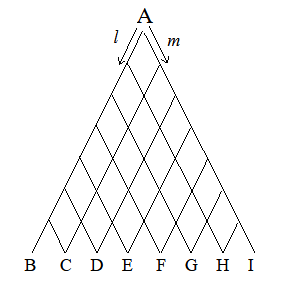
\includegraphics[width=0.95\columnwidth]{img/9.0 triangle.png}
\end{minipage}
\end{figure} 

\begin{thm}
    Фабрика окрашивает кубики в 6 цветов (каждую грань в свой цвет, набор цветов фиксирован). Сколько разновидностей кубиков можно изготовить?
\end{thm}

\begin{thm}
    На окружности даны 10 точек. Сколькими способами можно провести пять непересекающихся отрезков с концами в заданных точках?
\end{thm}

\begin{thm}
    Имеется прямоугольная доска $30 \times 40$. Найдите число прямоугольников, составленных из клеток этой доски.
\end{thm}

\begin{thm}
    У Кости есть $n$ друзей, и каждый день он приглашает некоторых из них в гости так, чтобы компания ни разу не повторялась (в какой-то день он может не пригласить никого). Сколько дней он сможет так делать?
\end{thm}

{\setlength{\intextsep}{2pt}
\begin{figure}[h]
\begin{minipage}{0.55\linewidth}\setlength{\parindent}{1.5em}
    \begin{thm}
    Сколькими способами можно добраться из пункта А
в пункт В по линиям сетки без самопересечений?
    \end{thm}
\end{minipage}
\hfill
\begin{minipage}{0.35\linewidth}\setlength{\parindent}{1.5em}
    A \begin{tabular}{ |m{.1em}|m{.1em}|m{.1em}|m{.1em}|m{.1em}|m{.1em}|m{.1em}|m{.1em}|m{.1em}|c| } 
    \hline
     & & & & & & & & & \\ 
    \hline
    \end{tabular} B
\end{minipage}
\end{figure}}

\begin{thm}
    Сколькими способами можно из последовательности 1, 2, ..., 2$n$ выбрать три числа, образующих арифметическую прогрессию?
\end{thm}

\begin{thm}
    У Вани есть кучка из 2012 морковок. Каждую минуту он произвольным образом делит одну из имеющихся у него кучек на две до тех пор, пока не получит 2012 кучек по одной морковке. При каждом делении Ваня записывает произведение числа морковок в получившихся двух кучках. Чему в результате равна сумма этих произведений?
\end{thm}

\begin{thm}
    Найдите количество клетчатых прямоугольников шахматной доски, содержащих клетку с4.
\end{thm}

\begin{thm}
    Сколько наборов целых чисел удовлетворяют условию:
    \par
    а) $0 < a_1 < a_2 < ... < a_n < n$; \hfill б) $0 \leq a_1 \leq a_2 \leq ... \leq a_n \leq n$? 
\end{thm}

\begin{thm}
    Сколько наборов целых неотрицательных чисел удовлетворяют условию:
    \par
    а) $a_1 + a_2 + ... + a_n = n$; \hfill б) $a_1 + a_2 + ... + a_n \leq n$? 
\end{thm}
\head{Ноябрь}{Ознакомительная самостоятельная работа по теме «Графы».}

\begin{thm}
    В кружке танцев каждая девочка познакомилась с 6 мальчиками и 7 девочками, а каждый мальчик -- с 3 девочками и 4 мальчиками. Кого в кружке больше: мальчиков или девочек?
\end{thm}

\begin{thm}
    Какие рисунки задают один и тот же граф? 
\end{thm}

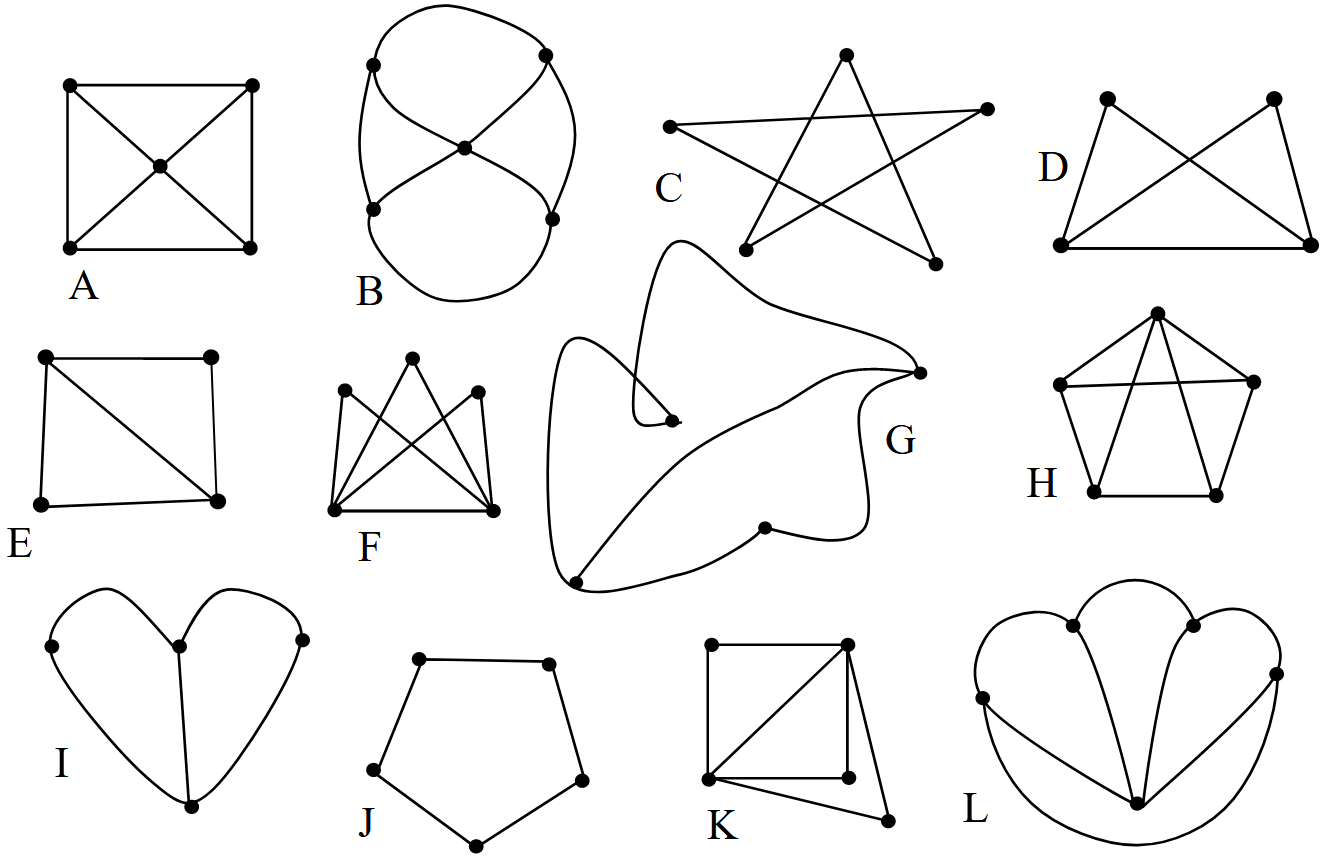
\includegraphics[width=0.95\columnwidth]{img/10.0.0 img1.png}

\begin{figure}[H]
\begin{minipage}{0.7\linewidth}
    \begin{thm}
        Докажите, что в любом графе с числом вершин не менее двух найдутся две вершины одинаковой степени.
    \end{thm}
\end{minipage}
    \hfill
\begin{minipage}{0.29\linewidth}
    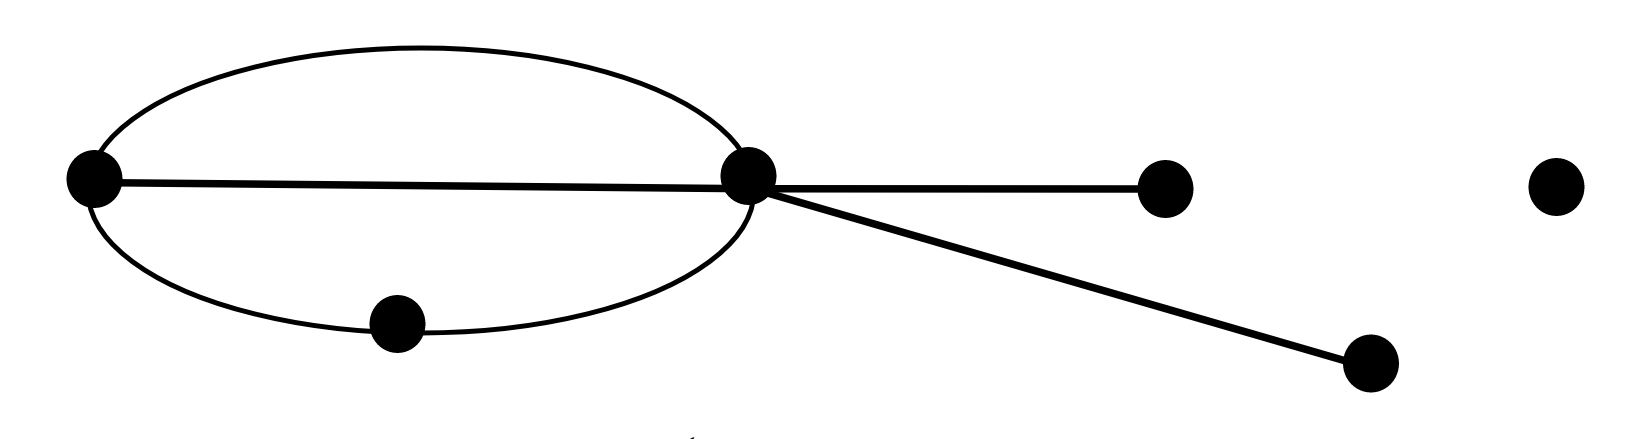
\includegraphics[width=0.95\columnwidth]{img/10.0.0 img2.png}
\end{minipage}
\end{figure}

\begin{thm}
    Запиши степени всех вершин графов $B$.
\end{thm}

\begin{thm}
    Проходит волейбольный турнир школы по круговой системе (каждая команда играет с каждой ровно один раз). Участвует 17 команд. В том числе и команда 8 класса. В некоторый момент времени оказалось, что все команды (кроме команды 8) сыграли разное количество матчей. Сколько матчей к этому моменту сыграла команда 8 класса?
\end{thm}

\begin{thm}
    В стране Миллениум некоторые города связаны между собой авиалиниями. Из столицы выходит 2013 авиалиний, из города Тьма--Таракань -- одна, а из всех остальных городов -- ровно по 2012 авиалинии. Можно ли из Тьмы--Таракани добраться в столицу?
\end{thm}

\begin{thm}
    В графе $n$ вершин. Степень каждой из них не меньше $\dfrac{n - 1}{2}$. Докажите, что граф связен.
\end{thm}

\begin{thm}
    В однокруговом турнире по настольному теннису каждый участник одержал четыре победы. Сколько человек участвовало в турнире?
\end{thm}

\begin{thm}
    Дайте определение эйлерова графа.
\end{thm}
\chapter{Графы}


\section{Подсчёт рёбер, двудольные графы, независимые множества.}

Как уже выводилось ранее, удвоенное количество ребер равно сумме всех степеней вершин графа. Часто идея подсчёта рёбер помогает решить задачу. Одна из идей состоит в подсчете концов рёбер (которая как раз и равна сумме степеней всех вершин). Лемма о рукопожатиях именно так и доказывается. Обобщением этой идеи является подсчёт концов рёбер двумя способами. Часто такая идея применяется, если рассматриваемый граф -- \textit{двудольный}.

\begin{dfn}
    Граф двудольный, если его множество вершин можно разбить на два подмножества так, что все рёбра будут соединять только элементы разных подмножеств.
\end{dfn}

\begin{thm}
    По окончании конкурса бальных танцев, в котором участвовали 7 мальчиков и 8 девочек, каждый назвал количество своих партнеров / партнёрш:3, 3, 3, 3, 3, 5, 6, 6, 6, 6, 6, 6, 6, 6, 6. Не ошибся ли кто--нибудь из них?
\end{thm}

\begin{prf}
    Рассмотрим граф, в котором вершины соответствуют танцорам, и две вершины соединены ребром, если они были партнёрами в танце. Ясно, что такой граф будет двудольным, в одной доле мальчики, в другой -- девочки. Количество партнёров / партнёрш, которое было названо -- это степень соответствующей вершины. Значит, эти степени можно разбить на два подмножества, степени доли мальчиков и степени доли девочек. Ясно, что число концов рёбер доли мальчиков в сумме равно числу концов рёбер доли девочек. Если степень 5 принадлежит одной доле, то к другой доле относятся степени 3 или 6, все они делятся на 3, поэтому сумма степеней одной доли делится на 3, а другой не делится. Следовательно, кто--то ошибся.  
\end{prf}

Часто подсчитывается не число рёбер, а число пар, троек и т.д. рёбер выходящих из одной вершины, как в следующем примере.

\begin{thm}
    Кружок по астрономии проводился в школе 20 раз. На каждое занятие приходило 5 человек. Известно, что никакие 2 школьника не встречались более чем на одном занятии. Доказать, что не менее 20 школьников посетили кружок.
\end{thm}

\begin{prf}
    Предположим, что это не так, и пусть школьников было не более 20. Рассмотрим двудольный граф, в верхней доле которого находятся вершины--школьники, а в нижней находятся вершины--занятия. Соединим их, если школьник посетил соответствующее занятие. Посчитаем число пар школьников двумя способами. С одной стороны их не более $\dfrac{20 \times 19}{2} = 190$. С другой стороны это число равно числу пар рёбер выходящих из вершины в нижней доле (занятия), т.е. их $20 \times (\dfrac{4 \times 5}{2}) = 200$. Противоречие.
\end{prf}

Иногда считается количество ребер, выходящих из какого--либо множества.

\begin{dfn}
    Назовем \textit{независимым} множеством вершин графа такое множество его вершин, что никакие две из них не соединены ребром.
\end{dfn}

\begin{dfn}
    Назовем \textit{доминирующим} множеством такое множество D вершин графа, что любая вершина соединена ребром с вершиной из D.
\end{dfn}

\begin{dfn}
    \textit{Максимальное} независимое множество вершин -- независимое множество вершин, которое становится зависимым при добавлении любой вершины.
\end{dfn}

С помощью подсчёта ребер можно доказать следующее утверждение.

\fbox{\begin{varwidth}{0.95\textwidth}
    \textbf{Теорема.} Если степени всех вершин в графе G не превосходят $l$, то число элементов в любом максимальном независимом множестве не меньше $\dfrac{V}{l + 1}$.
\end{varwidth}}

\textbf{Идеи доказательства.} Если I это максимальное независимое множество, то из I существует ребро
\\ к любой вершине из J -- дополнения к I. Значит $V = |I| + |J| \leq |I| + l |I|$.
\\  
Отсюда уже выводится требуемое неравенство.    
\head{Ноябрь}{Листок 10. Графы. Теория 1.}

\epigraph{\textit{«Бамбук -- дерево, ёжик -– дерево, ёжики с бамбуком –- лес...»}}

\textbf{\textit{Напоминание.}} Связный граф, не имеющий циклов, называется \textit{деревом}.

\fbox{\begin{varwidth}{0.95\textwidth}
    \textbf{\textit{Лемма.}} Граф является деревом тогда и только тогда, когда каждые две его вершины соединены ровно одним путём с различными ребрами.
\end{varwidth}}

\textit{\underline{Замечание}}: иногда дерево определяют именно как граф, в котором любые две вершины соединены ровно одним путём с различными ребрами (т.е. простым путём).

\begin{dfn}
    Вершина, из которой выходит только одно ребро, называется \textit{висячей}.
\end{dfn}

\fbox{\begin{varwidth}{0.95\textwidth}
    \textbf{\textit{Лемма о висячей вершине.}} В любом дереве найдётся висячая вершина.
\end{varwidth}}

\begin{dok}
    Выберем произвольную вершину А и рассмотрим какое--нибудь выходящее из этой вершины ребро. Пусть это ребро АВ. Если из вершины В не выходит других рёбер, то эта вершина –- искомая. В противном случае отметим ребро АВ и продолжим наш путь по любому неотмеченному ребру, выходящему из вершины B и так далее. Заметим, что в строящемся таким образом пути ни одна вершина не встречается дважды, в противном случае получился бы цикл, а дерево циклов не имеет. Поэтому при наличии неотмеченных рёбер мы будем каждый раз переходить в новую вершину, а их конечное число. Следовательно, в конце концов наш путь закончится. Но закончиться он может только в висячей вершине.
\end{dok}

\fbox{\begin{varwidth}{0.95\textwidth}
    \textbf{\textit{Утверждение.}} Число вершин дерева на единицу больше числа его рёбер.
\end{varwidth}}

\begin{thm}
    В стране Древляндии 2012 городов, некоторые из которых соединены дорогами. При этом любые два города соединяет ровно один маршрут. Сколько в этой стране дорог?
\end{thm}

\begin{prf}
    Поскольку любые два города соединяет ровно один маршрут (т.е. путь), то граф дорог этой страны – дерево. Поэтому рёбер (дорог) на единицу меньше, чем вершин. Следовательно вершин 2011.
\end{prf}

\begin{dfn}
    Граф О называется \textit{остовом} связного графа G, если О имеет те же вершины, что и G, получается из G удалением некоторых рёбер, и является деревом.
\end{dfn}

\fbox{\begin{varwidth}{0.95\textwidth}
    \textbf{\textit{Лемма об остове.}} Любой связный граф имеет остов.
\end{varwidth}}

\begin{dok}
    Если граф уже является деревом, то в качества остова можно выбрать его самого. Пусть данный граф не является деревом. Тогда докажем, что в любом таком графе мы можем удалить одно ребро без потери связности. Действительно, если этот граф не дерево, то в нём есть цикл. Удалим в цикле одно ребро. Очевидно, что граф останется связным. Поскольку если две вершины были соединены путём, не проходящим через удалённое ребро, то для них ничего не изменилось. Если же путь проходил через удалённое ребро, то заменим это ребро путём по оставшемуся куску цикла. Следовательно, путь восстановлен и граф остался связным. Таким образом, можно удалять по одному ребру до тех пор, пока граф не станет деревом. Но тогда мы получим искомый остов.
\end{dok}

\begin{figure}[H]
\begin{minipage}{0.65\linewidth}\setlength{\parindent}{1.5em}
    \begin{ques}
     Может ли граф иметь несколько остовов?
    \end{ques}

    \begin{thm}
    Рома и Саша стирают у фигуры, приведённой на рисунке по одной стороне квадратиков. Нельзя стирать вершины квадратиков и сторону так, чтобы фигура распалась на две несвязные части. Кто выигрывает в эту игру, если начинает Рома?
    \end{thm}
\end{minipage}
\hfill
\begin{minipage}{0.3\linewidth}

        \begin{tabular}{ | m{0em} | m{0em} | m{0em} | m{0em} | m{0em} | m{0em} | m{0em} | m{0em} | } 
    \hline
   &  &  &  &  &  &  &  \\ 
     \hline
   &  &  &  &  &  &  &  \\ 
    \hline
   &  &  &  &  &  &  &  \\ 
    \hline
   &  &  &  &  &  &  &  \\ 
    \hline
   &  &  &  &  &  &  &  \\ 
    \hline
\end{tabular}
    
\end{minipage}
\end{figure} 

\begin{prf}
    У данной фигуры $8 \times 6 + 9 \times 5 = 93$ стороны маленьких квадратиков (ребер графа) и $6 \times 9 = 54$ вершины. Не получится стереть сторону лишь тогда, когда граф станет деревом. Но тогда при 54 вершинах должно будет остаться 53 ребра. Поэтому при любых ходах стереть можно ровно 40 отрезков и выиграет Саша, поскольку именно он делает чётные ходы. \textbf{\textit{Ответ}}: выиграет Саша
\end{prf}
\head{Ноябрь}{Листок 10. Графы. Теория 2.}

\section{Эйлеровы и гамильтоновы обходы. Ориентированные графы.}

\begin{dfn}
    Граф называется \textit{эйлеровым}, если в нем существует цикл, проходящий по всем ребрам по одному разу, так называемый \textit{эйлеров цикл}. \textit{Полуэйлеров} (или \textit{почти эйлеров}) граф -- граф, в котором есть путь, проходящий по одному разу по каждому ребру.
\end{dfn}

\textit{\underline{Замечание}}: в частности любой эйлеров граф является почти эйлеровым, т.к. любой цикл является путём. Примером почти эйлеровых графов являются фигуры, которые можно нарисовать, не отрывая карандаша от бумаги и не проводя карандаш повторно по каким-либо линиям. 

\fbox{\begin{varwidth}{0.95\textwidth}
    \textbf{Теорема Эйлера (критерий эйлеровости графа)}. Граф эйлеров тогда и только тогда, когда он связен, и все его вершины имеют чётную степень. Граф полуэйлеров тогда и только тогда, когда он связен и имеет не более двух вершин с нечётной степенью.
\end{varwidth}}

\begin{dfn}
    Граф называется \textit{гамильтоновым}, если в нём существует замкнутый путь, проходящий через все вершины ровно по одному разу. Такой путь, соответственно, называют \textit{гамильтоновым} \textit{циклом}.
\end{dfn}

% \begin{figure}[H]
% \begin{minipage}{0.65\linewidth}\setlength{\parindent}{1.5em}
%     Многие головоломки сводятся к эйлеровости или гамильтоновости определенных графов. Эйлер придумал свою теорему в 1736 году в связи с задачей об обходе кенигсбергских мостов. Именно с теоремы Эйлера теория графов отсчитывает свою историю. Гамильтоновы путь, цикл и граф названы в честь ирландского математика сэра Уильяма Гамильтона, который в 1859 году впервые определил эти классы, исследовав задачу «кругосветного путешествия» по додекаэдру, узловые вершины которого символизировали крупнейшие города Земли, а рёбра – соединяющие их дороги. Играющий должен обойти все города и вернуться в исходный. 
% \end{minipage}
% \hfill
% \begin{minipage}{0.3\linewidth}
%     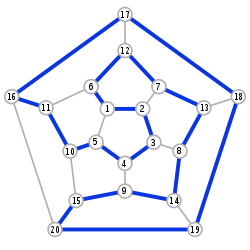
\includegraphics[width=0.95\columnwidth]{img/10.2 1 pyat.png}
% \end{minipage}
% \end{figure} 

\begin{wrapfigure}{R}{0.35\textwidth}
\centering
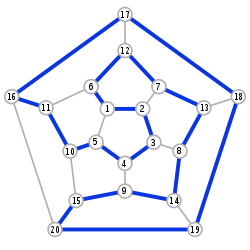
\includegraphics[width=0.3\textwidth]{img/10.2 1 pyat.png}
\end{wrapfigure}

Многие головоломки сводятся к эйлеровости или гамильтоновости определенных графов. Эйлер придумал свою теорему в 1736 году в связи с задачей об обходе кенигсбергских мостов. Именно с теоремы Эйлера теория графов отсчитывает свою историю. Гамильтоновы путь, цикл и граф названы в честь ирландского математика сэра Уильяма Гамильтона, который в 1859 году впервые определил эти классы, исследовав задачу «кругосветного путешествия» по додекаэдру, узловые вершины которого символизировали крупнейшие города Земли, а рёбра – соединяющие их дороги. Играющий должен обойти все города и вернуться в исходный. Справедливости ради следует отметить, что уже до этого была задача, сводящаяся к гамильтоновости некоторого графа, а именно задача обхода конем всех полей шахматной доски с возвращением в исходную клетку. Эта задача была в своё время успешно решена Эйлером. На рисунке изображен граф додекаэдра Гамильтона.

\begin{figure}[H]\begin{minipage}{0.3\linewidth}
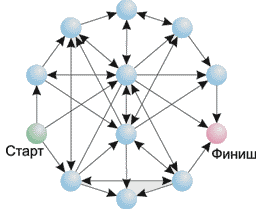
\includegraphics[width=0.95\columnwidth]{img/10.2curse.png}
\end{minipage}
\hfill
\begin{minipage}{0.69\linewidth}\setlength{\parindent}{1.5em}
    \begin{dfn}
    Пусть $n$ -- количество вершин в данном графе. Если степень каждой вершины не менее, чем $\dfrac{n}{2}$, то граф называется \textit{графом Дирака}.
    \end{dfn}
    \begin{ques}
        Почему граф Дирака связен?
    \end{ques} 
    (На рисунке изображён граф из задачи поиска гамильтонова пути с помощью ДНК--вычислений.)
    \\
    Для гамильтоновости графов в отличие от эйлеровости не найдено простых критериев. Тем не менее существует много достаточных условий. Приведём некоторые из них.
\end{minipage}
\end{figure}

\fbox{\begin{varwidth}{0.95\textwidth}
    \textbf{Теорема Поша.} Пусть граф имеет p вершин, где $p \geq 3$. Если для всякого $n$ такого, что $1 \leq n \leq \dfrac{p - 1}{2}$, число вершин со степенями, не превосходящими $n$, меньше чем $n$, и для нечётного $p$ количество вершин степени $\dfrac{p - 1}{2}$ не превосходит $\dfrac{p - 1}{2}$, то такой граф гамильтонов.
    \\
    \textbf{Теорема Оре.} Если граф имеет $p$ вершин, где $p > 2$ и сумма степеней несмежных вершин не меньше $p$, то граф гамильтонов. 
    \\ 
    \textbf{Теорема Дирака.} Если граф имеет $p$ вершин, где $p > 2$ и степень любой вершины не меньше $\dfrac{p}{2}$, то граф гамильтонов.
\end{varwidth}}

\newpage

\begin{ques}
    Является ли дерево эйлеровым графом?
\end{ques}

\begin{ques}
    Является ли дерево гамильтоновым графом?
\end{ques}

\begin{dfn}
    Граф называется \textit{двусвязным}, если между любыми двумя вершинами существует два непересекающихся по вершинам (кроме начала и конца) пути.
\end{dfn}

\textit{\textbf{Утверждение.}} Гамильтонов граф двусвязен.

\begin{dfn}
    \textit{Тэта-графом} называется граф из двух вершин степени 3 и трёх непересекающихся простых путей, соединяющих их, причём длина каждого из путей не меньше 2.
\end{dfn}

\fbox{\begin{varwidth}{0.95\textwidth}
    \begin{thrm}
        Каждый негамильтонов двусвязный граф содержит тэта--подграф.
    \end{thrm}
\end{varwidth}}

Задачи, в которых нужно доказать отсутствие гамильтонова цикла, часто сводятся к поиску инварианта или какой-нибудь величины на вершинах, которая известным образом изменяется при переходе от вершины к смежной вершине. Как, например, шахматная раскраска в следующем примере.

\begin{thm}
    Докажите, что шахматный конь не может обойти доску 5 на 5 и вернуться в исходную клетку.
\end{thm}

\begin{prf}
    Каждым ходом конь встаёт на клетку другого цвета. Так как всего ходов 25 -- нечётное число, то последним ходом он должен встать на клетку, не совпадающую по цвету с начальной. Противоречие.
\end{prf}

\begin{dfn}
    Граф, в котором рёбра снабжены стрелками, называется ориентированным. Полный граф, в котором каждое ребро снабжено ориентацией (стрелкой), называется \textit{полным ориентированным графом }или \textit{турниром}.
\end{dfn}

\begin{dfn}
    \textit{Исходящей степенью} вершины в ориентированном графе называется количество рёбер, выходящих из данной вершины. \textit{Входящей степенью} вершины в ориентированном графе называется количество рёбер, входящих в данную вершину.
\end{dfn}
\hfill \break
Заметим следующий общий факт. Так как каждое ориентированное ребро имеет одно начало и один конец, то сумма всех исходящих степеней вершин равна количеству рёбер. Аналогично каждое ребро имеет один конец, поэтому сумма входящих степеней вершин равна количеству рёбер. Потому сумма исходящих степеней вершин равна сумме входящих степеней вершин.

\begin{thm}
    В однокруговом турнире по настольному теннису каждый участник одержал четыре победы. Сколько человек участвовало в турнире? (Ничьих в теннисе не бывает).
\end{thm}

\begin{prf}
    Обозначим участников за вершины графа. Если участник A выиграл у участника B, поставим стрелку от A к B. Переформулировка на язык графов: «В полном ориентированном графе из каждой вершины выходит четыре ребра. Сколько в нём вершин?».
    \\
    Пусть всего в графе $x$ вершин, у каждой из которых исходящая степень 4. Сумма исходящих степеней вершин -- $4x$, сумма входящих -- такая же. Так как общая степень каждой вершины одна и та же и равна $x – 1$, а исходящая равна 4, то входящая степень у всех вершин тоже одинакова. Значит, она тоже равна 4. Отсюда $x
    – 1 = 8$, и в турнире принимало участие 9 человек.
\end{prf}
\head{Ноябрь}{Листок 10. Теория графов. Подсчет рёбер и лемма Холла.}

\begin{thm}
    В шахматном турнире в один круг участвуют 11 шахматистов. В настоящее время среди любых трёх из них хотя бы двое ещё не сыграли. Доказать, что сыграно не более 30 партий.
\end{thm}

\begin{thm}
    У каждого из жителей города $N$ знакомые составляют не менее 30\% населения города. На выборы каждый из жителей ходит, только если баллотируется хотя бы один его знакомый. Доказать, что можно так провести выборы из двух кандидатов, что на них придёт не менее половины жителей.
\end{thm}

\begin{thm}
    В стране 1993 города, и из каждого выходит не менее 93 дорог. Известно, что из любого города можно проехать по дорогам в любой другой. Доказать, что это можно сделать с не более чем 62 пересадками.
\end{thm}

\begin{thm}
    В некотором парламенте 1600 депутатов, которые образовали 16000 комитетов, в каждом из которых не менее 80 депутатов. Доказать, что существуют два комитета, имеющие не менее 4 общих членов.
\end{thm}

\begin{thm}
    В некоторые 16 клеток доски 88 поставили по ладье. Какое наименьшее количество пар бьющих друг друга ладей могло при этом оказаться?
\end{thm}

\begin{thm}
    \textbf{Лемма Холла:} пусть есть двудольный граф $G$ с двумя долями -- верхней $U$ и нижней $V$. Через $v(X)$, где $X$ -- подмножество верхней доли, будем обозначать множество элементов в нижней доле инцидентных с $M$. Пусть для любого подмножества $X$ верхней доли верно, что $v(X) \geq |X|$. Доказать, что в таком случае в графе существует полное паросочетание, т.е. для каждой вершины верхней доли можно выбрать вершину нижней доли, соединённую с ней так, что никакие две выбранные вершины не совпадают.
\end{thm}

\begin{thm}
    Пусть есть двудольный граф такой, что его верхняя доля есть объединение множеств $A_1, A_2 ... A_k$, а $l_1, l_2 ...$ и $l_k$ -- фиксированные натуральные числа. Доказать, что если для любых $B_1, K B_k$, являющихся подмножествами $A_1, A_2 ... A_k$, верно, что $v(B_1) + K + v(B_k) \geq l_1 B_1 + K + l_k B_k$, то можно выбрать непересекающихся представителей для верхней доли, по $l_i$ для каждого элемента $A_i$.
\end{thm}

\begin{thm}
\begin{enumerate}[itemsep=0.05em]
    \item Доказать, что если в графе степени всех вершин не меньше $n$ и не больше $m$, то можно удалить часть рёбер так, что в полученном графе степени всех вершин будут заключены между $n - k$ и $m - k$.
    \item Доказать, что если в графе степени всех вершин не меньше $n$ и не больше $2n$, то можно удалить часть рёбер так, что в полученном графе степени всех вершин будут заключены между $m$ и $2m$, где $m$ от 1 до $n$. 
    \item Доказать то же самое если степени между $n$ и $kn$ для произвольного натурального $k$.
\end{enumerate}
\end{thm}

\begin{thm}
    В лагерь приехали пионеры. Каждый из них имеет от 50 до 100 знакомых. Доказать, что всем им можно выдать пилотки 1331 цвета так, что среди знакомых каждого найдётся 20 человек с разными цветами пилотки.
\end{thm}
\head{Декабрь}{Листок 10. Графы. Уровень 1.}

\section{Подсчёт рёбер, двудольные графы, независимые множества.}

Как уже выводилось ранее, удвоенное количество ребер равно сумме всех степеней вершин графа. Часто идея подсчёта рёбер помогает решить задачу. Одна из идей состоит в подсчете концов рёбер (которая как раз и равна сумме степеней всех вершин). Лемма о рукопожатиях именно так и доказывается. Обобщением этой идеи является подсчёт концов рёбер двумя способами. Часто такая идея применяется, если рассматриваемый граф -- \textit{двудольный}.

\begin{dfn}
    Граф двудольный, если его множество вершин можно разбить на два подмножества так, что все рёбра будут соединять только элементы разных подмножеств.
\end{dfn}

\begin{thm}
    По окончании конкурса бальных танцев, в котором участвовали 7 мальчиков и 8 девочек, каждый назвал количество своих партнеров / партнёрш:3, 3, 3, 3, 3, 5, 6, 6, 6, 6, 6, 6, 6, 6, 6. Не ошибся ли кто--нибудь из них?
\end{thm}

\begin{prf}
    Рассмотрим граф, в котором вершины соответствуют танцорам, и две вершины соединены ребром, если они были партнёрами в танце. Ясно, что такой граф будет двудольным, в одной доле мальчики, в другой -- девочки. Количество партнёров / партнёрш, которое было названо -- это степень соответствующей вершины. Значит, эти степени можно разбить на два подмножества, степени доли мальчиков и степени доли девочек. Ясно, что число концов рёбер доли мальчиков в сумме равно числу концов рёбер доли девочек. Если степень 5 принадлежит одной доле, то к другой доле относятся степени 3 или 6, все они делятся на 3, поэтому сумма степеней одной доли делится на 3, а другой не делится. Следовательно, кто--то ошибся.  
\end{prf}

Часто подсчитывается не число рёбер, а число пар, троек и т.д. рёбер выходящих из одной вершины, как в следующем примере.

\begin{thm}
    Кружок по астрономии проводился в школе 20 раз. На каждое занятие приходило 5 человек. Известно, что никакие 2 школьника не встречались более чем на одном занятии. Доказать, что не менее 20 школьников посетили кружок.
\end{thm}

\begin{prf}
    Предположим, что это не так, и пусть школьников было не более 20. Рассмотрим двудольный граф, в верхней доле которого находятся вершины--школьники, а в нижней находятся вершины--занятия. Соединим их, если школьник посетил соответствующее занятие. Посчитаем число пар школьников двумя способами. С одной стороны их не более $\dfrac{20 \times 19}{2} = 190$. С другой стороны это число равно числу пар рёбер выходящих из вершины в нижней доле (занятия), т.е. их $20 \times (\dfrac{4 \times 5}{2}) = 200$. Противоречие.
\end{prf}

Иногда считается количество ребер, выходящих из какого--либо множества.

\begin{dfn}
    Назовем \textit{независимым} множеством вершин графа такое множество его вершин, что никакие две из них не соединены ребром.
\end{dfn}

\begin{dfn}
    Назовем \textit{доминирующим} множеством такое множество D вершин графа, что любая вершина соединена ребром с вершиной из D.
\end{dfn}

\begin{dfn}
    \textit{Максимальное} независимое множество вершин -- независимое множество вершин, которое становится зависимым при добавлении любой вершины.
\end{dfn}

С помощью подсчёта ребер можно доказать следующее утверждение.

\fbox{\begin{varwidth}{0.95\textwidth}
    \textbf{Теорема.} Если степени всех вершин в графе G не превосходят $l$, то число элементов в любом максимальном независимом множестве не меньше $\dfrac{V}{l + 1}$.
\end{varwidth}}

\textbf{Идеи доказательства.} Если I это максимальное независимое множество, то из I существует ребро
\\ к любой вершине из J -- дополнения к I. Значит $V = |I| + |J| \leq |I| + l |I|$.
\\  
Отсюда уже выводится требуемое неравенство.    
\head{Декабрь}{Переводная самостоятельная работа. Уровень 1 $\Rightarrow$ уровень 2.}

\section{Подсчёт рёбер, двудольные графы. Обходы.}

\begin{figure}[H]
\begin{minipage}{0.19\linewidth}
    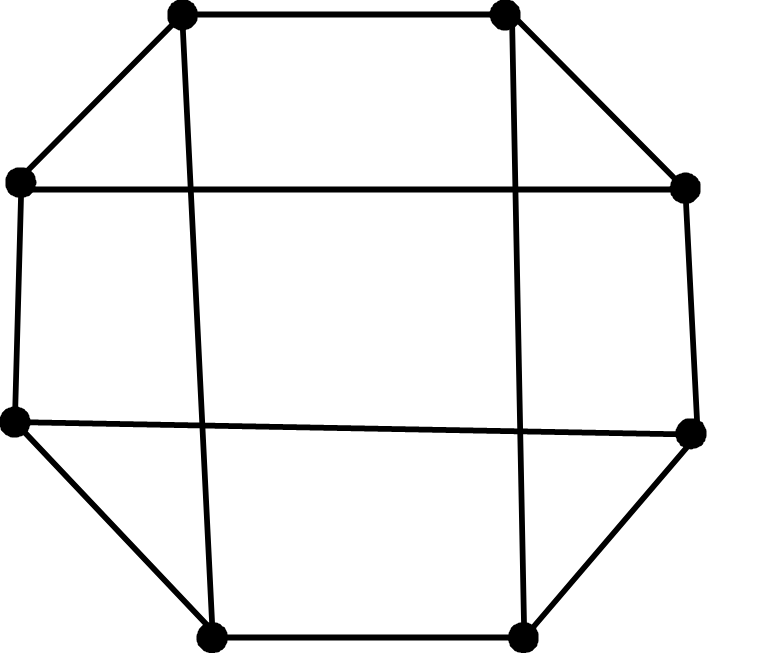
\includegraphics[width=0.95\columnwidth]{img/10.4.0 img1.png}
\end{minipage}
    \hfill
\begin{minipage}{0.8\linewidth}
    \begin{thm}
        Является ли граф, приведённый на рисунке, двудольным?
    \end{thm}
    \begin{thm}
        На конкурсе по математике было 20 задач. На разбор пришло 20 школьников. Известно, что каждый школьник решил ровно две задачи и каждую задачу решило ровно два школьника. Докажите, что можно так организовать разбор задач, что каждую задачу расскажет решивший её школьник.
    \end{thm}
\end{minipage}
\end{figure}

\begin{figure}[H]
\begin{minipage}{0.6\linewidth}
    \begin{thm}
        На рисунке изображён план дома. Линиями отмечены стены. (см. рис.) Можно ли провести по дому освещение (протянуть один провод) так, чтобы при этом просверлить каждую стену ровно один раз?
    \end{thm}
    \begin{thm}
        В одном учреждении каждый сотрудник выписывает две газеты, каждую газету выписывают пять человек, каждую пару газет выписывает только один человек. Сколько человек в учреждении и сколько они выписывают газет?
    \end{thm}
\end{minipage}
    \hfill
\begin{minipage}{0.39\linewidth}
    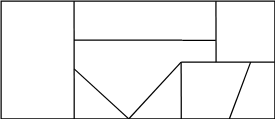
\includegraphics[width=0.95\columnwidth]{img/10.4.0 img2.png}
\end{minipage}
\end{figure}

\begin{thm}
    Докажите, что если граф двудольный, то все его циклы состоят из чётного числа рёбер.
\end{thm}

\begin{thm}
    Докажите, что если в графе все циклы чётной длины, то этот граф -- двудольный.
\end{thm}

\begin{thm}
    В стране Карликании 11 городов. Известно, что среди любых трёх из них хотя бы двое ещё не соединены авиалинией. Докажите, что в стране не более 30 авиалиний.
\end{thm}

\begin{thm}
    Докажите, что независимое множество максимально тогда и только тогда, когда оно доминирующее.
\end{thm}

\begin{thm} $^*$
    Докажите теорему из листка с теорией, воспользовавшись подсказкой.
\end{thm}

\begin{thm}
    В шахматном турнире в один круг участвуют 11 шахматистов. В настоящее время среди любых трёх из них хотя бы двое еще не сыграли. Доказать, что сыграно не более 30 партий.
\end{thm}

\begin{thm}
В классе каждый мальчик дружит ровно с двумя девочками, а девочка -- ровно с тремя мальчиками. Ещё известно, что в классе 31 пионер и 19 парт. Сколько человек в классе?
\end{thm}

\begin{thm}
    В народной дружине 100 человек. В каждый вечер на дежурство выходят трое. Докажите, что нельзя составить график дежурств таким образом, что любые два человека будут дежурить вместе ровно один раз.
\end{thm}

\begin{thm}
    Кружок по астрономии проводился в школе 20 раз. На каждое занятие приходило 6 человек. Известно, что никакие два школьника не встречались более чем на одном занятии. Доказать, что не менее 21 школьника посетили кружок.
\end{thm}

\begin{figure}[H]
    \begin{minipage}{0.89\linewidth}\setlength{\parindent}{1.5em}
        \begin{thm}
             В некоторые 16 клеток доски 8×8 поставили по ладье. Какое наименьшее количество пар бьющих друг друга ладей могло при этом оказаться?
        \end{thm}
        \begin{thm}
            На рисунке изображён план парка и его окрестностей, линиями отмечены заборы. (см. рис.) Можно ли прогуляться по парку так, чтобы при этом перелезть через каждый забор ровно один раз?
        \end{thm}
    \end{minipage}
\hfill
    \begin{minipage}{0.1\linewidth}
        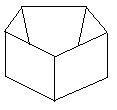
\includegraphics[width=0.95\columnwidth]{img/10.4 figure.png}
    \end{minipage}
\end{figure}

\begin{thm}
    В футбольном турнире участвует 20 команд. После того, как все команды провели по две игры, организаторы турнира решили разбить их на три дивизиона, но так, чтобы в одном дивизионе не было команд, уже игравших друг с другом. Всегда ли они смогут это сделать? (Подсказка. Вспомните теорему о циклических графах)
\end{thm}

\begin{thm}
    На $n$ карточках с двух сторон написаны числа от 1 до $n$ по два раза каждое. Докажите, что карточки можно положить на стол так, чтобы сверху каждое из чисел было написано ровно один раз.
\end{thm}

\begin{thm} $^*$
    В некоторой стране из каждого города выходит по три железные дороги. Две компании хотят их все приватизировать. Антимонопольный комитет требует, чтобы из каждого города выходили дороги обеих компаний. Докажите, что компании могут договориться так, чтобы требование антимонопольного комитета было выполнено.
\end{thm}

\begin{thm}
    Сварщик варит решетку размером 4×4 из кусков ломаных. Сможет ли он это сделать, если у него есть а) 5 ломаных длины 8; б) 8 ломаных длины 5? \textit{(Форма ломаных может быть различной)}
\end{thm}
\head{Январь}{Листок 10. Графы. Уровень 3.}

\section{Деревья. Изоморфные графы.}

\begin{thm}
    Докажите, что граф является деревом тогда и только тогда, когда каждые две его вершины соединены ровно одним путём с различными ребрами.
\end{thm}

\begin{thm}
    В некотором графе все вершины имеют степень три. Докажите, что в нём есть цикл.
\end{thm}

\begin{thm}
    а) Докажите, что в дереве с $n \geq 2$ вершинами найдутся хотя бы две висячие вершины. 
    \par б) Можете ли вы привести пример графа со 101 вершиной, из которых 100 висячих?
\end{thm}

\begin{thm}
    Ребра дерева окрашены в два цвета. Если в какой-то вершине сходятся ребра одного цвета, то можно их все перекрасить в другой цвет. Можно ли всё дерево сделать одноцветным?
\end{thm}

\begin{thm}
    Будем красить в два цвета не рёбра, а вершины графа. Можно ли любое дерево раскрасить так, что любое ребро будет соединять вершины разных цветов?
\end{thm}

\begin{thm}
    Волейбольная сетка имеет вид прямоугольника размером 60х600 клеток. Хулиган Лёша хочет разрезать как можно больше верёвочек так, чтобы сетка не распалась на отдельные куски. Сколько веревочек ему удастся разрезать?
\end{thm}

\begin{thm}
    На планете Абра-Кадабра 100 государств, некоторые из которых соединены авиалиниями. Известно, что из любого государства можно попасть в любое другое (возможно, с пересадками). Докажите, что можно совершить кругосветное путешествие (побывать в каждой стране), сделав не более 196 перелётов.
\end{thm}

\begin{thm}
    Докажите, что в любом связном графе можно удалить вершину вместе со всеми выходящими из неё ребрами так, чтобы он остался связным.
\end{thm}

\begin{thm}
    В группе из нескольких человек некоторые люди знакомы друг с другом, а некоторые нет. Каждый вечер один из них устраивает ужин для всех своих знакомых, на котором знакомит их друг с другом. После того, как каждый человек устроил хотя бы по одному ужину, оказалось, что какие--то два человека вcё ещё не знакомы. Докажите, что они не познакомятся и на следующем ужине.
\end{thm}

\begin{dfn}
    Два графа называются \textit{изоморфными}, если у них поровну вершин, и если  вершины каждого графа можно занумеровать числами от 1 до $n$ так, что вершины $k$ и $l$ соединены ребром в одном графе тогда и только тогда, когда соединены ребром вершины $k$ и $l$ в другом графе.
\end{dfn}

\begin{thm}
    Верно ли, что два графа изоморфны, если
        \begin{enumerate}[noitemsep, label=\asbuk*), ref=\asbuk*]
            \item у них по 10 вершин, степень каждой из которых равна 9?
            \item у них по 8 вершин, степень каждой из которых равна 3, и нет петель?
            \item они связны, без циклов и петель, содержат 5 вершин и 4 ребра?
        \end{enumerate}
\end{thm}

\begin{thm}
    В связном графе степени четырёх вершин равны 3, а степени остальных равны 4. Докажите, что нельзя удалить одно ребро так, чтобы этот граф распался на две изоморфные компоненты связности.
\end{thm}

\begin{thm} $^*$
    Маша нарисовала на доске 7 графов, каждый из которых является деревом с шестью вершинами. Докажите, что среди них найдутся, по крайней мере, два изоморфных.
\end{thm}

\head{Февраль}{Листок 10. Графы. Уровень 4.}

\section{Эйлеровы и гамильтоновы обходы. Ориентированные графы.}

\begin{thm}
    Доказать, что в графе, соответствующем задаче про коней из листка с теорией есть гамильтонов путь.
\end{thm}

\begin{ex}
    Изобразите на додекаэдре гамильтонов цикл.
\end{ex}

\begin{thm}
    В большой книге предсказаний Глеба Лобы написано:
    \begin{enumerate}[itemsep=0.05em]
        \item Если сегодня дождь, то завтра будет солнце.
        \item Если сегодня снег, то завтра дождь.
        \item Если сегодня холод, то завтра будет ветер.
        \item Если сегодня солнце, то завтра будет тепло
        \item Если сегодня тепло, то завтра будет холодно.
        \item Если сегодня холодно, то завтра будет пасмурно.
        \item Если сегодня ветер, то завтра будет снег.
        \item Если сегодня пасмурно, то завтра будет дождь.
    \\ Оказалось, что в январе все предсказания сбылись. 1 января были ветер и солнце. Какая погода была 5 января?
    \end{enumerate}
\end{thm}

\begin{thm}
    В однокруговом шахматном турнире один шахматист заболел и не доиграл свои партии. Всего в турнире было проведено 24 встречи. Сколько шахматистов участвовало в турнире, и сколько партий сыграл выбывший участник?
\end{thm}

\begin{thm}
    Докажите, что на рёбрах любого связного графа можно так расставить стрелки, что найдётся вершина, из которой можно было бы добраться по стрелкам в любую другую.
\end{thm}

\begin{thm}
    Сумасшедший король хочет ввести на дорогах своего королевства одностороннее движение так, чтобы, выехав из одного города, уже будет нельзя в него вернуться. Удастся ли ему осуществить свою затею, если в его государстве любые два города соединены дорогой?
\end{thm}

\begin{thm}
    В некоторой стране каждый город соединён с каждым дорогой с односторонним движением. Докажите, что найдётся город, из которого можно попасть в любой другой.
\end{thm}

\begin{thm}
    В одном государстве 100 городов и каждый соединён с каждым дорогой с односторонним движением. Докажите, что можно поменять направление движения на одной дороге так, что из любого города можно будет доехать до любого другого.
\end{thm}

\begin{thm}
    Ученики одного класса сыграли между собой круговой турнир по настольному теннису. Будем говорить, что игрок А сильнее игрока В, если либо А выиграл у В, либо существует игрок С, у которого А выиграл, а В ему проиграл.
    \\ а) Докажите, что есть игрок, которых сильнее всех.
    \\ б) Докажите, что игрок, выигравший турнир, сильнее всех. (\underline{\textit{Замечание:}} в теннисе ничьих не бывает)
\end{thm}

% \begin{thm}
%     Докажите, что шахматный конь может обойти доску $4 \times n$, побывав в каждой клетке по одному разу. Может ли он при этом вернуться в исходную клетку?
% \end{thm}

\begin{thm}
    При дворе короля Артура собрались $2n$ рыцарей, причём каждый из них имеет среди присутствующих не более $n - 1$ врага. Доказать, что Мерлин может так рассадить рыцарей за круглым столом, что ни один из них не будет сидеть рядом с врагом.
\end{thm}

\begin{thm}
    Докажите, что гамильтонов граф двусвязен.
\end{thm}

\begin{thm} $^*$
    Докажите теорему Поша.
\end{thm}

\begin{thm} $^*$
    Выведите теоремы Дирака и Оре из теоремы Поша.
\end{thm}

\begin{thm}
    Докажите, что в двусвязном негамильтоновом графе содержится тэта--граф в качестве подграфа.
\end{thm}
\head{Февраль}{Листок Весёлый.}

\textit{Для поднятия настроения и «боевого духа» в качестве бонуса для тех, кто раньше всех успешно
справился с предыдущим листком.}

\begin{thmF}
    Однажды король призвал ко двору четырёх великих мудрецов. Он собрал их всех в своём тронном зале и показал им 7 золотых табличек. На первой было написано число 1, на второй 2, ..., на седьмой 7. Затем он объявил мудрецам, что каждый из них получит одну из этих табличек. После чего он перемешал таблички и дал каждому мудрецу по одной. Таким образом, каждый мудрец знал, какое число досталось ему, но не знал, какие числа достались другим. Раздав таблички, король спросил первого мудреца: 
    \par -- Твоё число больше чем числа других мудрецов?
    \par -- Я не знаю, -- ответил первый мудрец. 
    \\ Затем король спросил второго мудреца: 
    \par -- Твоё число больше, чем числа других мудрецов?
    \par -- Я не знаю, -- ответил второй мудрец.
    \\ Король спросил третьего мудреца: 
    \par -- Твоё число больше, чем числа других мудрецов? 
    \par -- Я не знаю, -- ответил третий мудрец.
    \\ Наконец спросил король четвёртого мудреца: 
    \par -- Твоё число больше чем числа других мудрецов?
    \par -- Да, -- ответил тот. 
    \par -- Ты уверен в этом? -- переспросил его король. 
    \par -- Совершенно уверен. Более того, про каждого из мудрецов я точно знаю, какое число ему досталось.
    \\ Подивился король уму своих мудрецов, однако нас их ответы не должны удивлять. Определите про каждого из мудрецов, какое число ему досталось. 
\end{thmF}
{\footnotesize \textit{(Важное пояснение к задаче: про каждого из мудрецов общеизвестным является то, что он обладает совершенным интеллектом, то есть мгновенно может из имеющейся у него информации сделать все логические выводы)}}

\begin{figure}[h]
    \begin{minipage}{0.75\linewidth}
        \begin{thmF}
            Маша положила на стол несколько отрезков и обнаружила четыре квадрата, все стороны которых лежат на этих отрезках. Все четыре квадрата были разных размеров. (Пример такого расположения отрезков показан на рисунке.) Докажите, что Маша может переложить отрезки так, чтобы квадратов оказалось шесть (и все разных размеров).
        \end{thmF}
    \end{minipage}
\hfill
    \begin{minipage}{0.2\linewidth}
        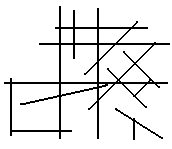
\includegraphics[width=0.95\columnwidth]{img/10.8.0 img1.png}
    \end{minipage}
\end{figure}

\begin{thmF}
    На выборах в Стране Чудаков можно было проголосовать за партию жуликов, партию воров или партию дураков (за какую--то одну). Всего бюллетеней было столько же, сколько избирателей, но некоторые избиратели не пришли, и их бюллетени оказались незаполненными. Тогда партия воров украла половину этих бюллетеней и заполнила в свою пользу. После этого при подсчёте голосов партии жуликов удалось присвоить треть голосов за каждую из остальных партий. В результате партия дураков набрала 25\% (от числа заполненных бюллетеней). Если бы выборы были честными, партия дураков набрала бы более 50\% от числа заполненных бюллетеней. Докажите, что явка на выборы была не более 60\%, если известно, что все бюллетени были заполнены правильно.
\end{thmF}
\chapter{Делимость целых чисел -- 2}
\head{Март}{Листок 11. Делимость целых чисел -- 2.}

\epigraph{\textit{Прошу -- забудь всё, чему ты учился в школе, потому что ты этому не научился.}}{\textit{Э.Ландау «Основы анализа»}}

\section{Часть 1.}

Если $a$ и $b \in \mathbb{Z}$, причём $b > 0$, то существует такое \textit{q (частное)} $\in \mathbb{Z}$, что $a = bq + r$, где \textit{r (остаток)} $\in \mathbb{Z}$ и $0 \leq r < b$. Числа $q$ и $r$ определяются по данным $a$ и $b$ единственным образом: если $r = 0$, мы получаем случай, когда $a$ делится на $b$. В этом случае $b$ называют \textit{делителем} $a$.
\\ Пусть $a$ и $b$ -- два целых числа, не равные одновременно нулю. Рассмотрим все числа, на которые делятся и $a$ и $b$ одновременно, т.е. рассмотрим все \textit{общие делители} $a$ и $b$. Выберем из них наибольший и назовем его \textit{наибольшим общим делителем}. Дальше будем обозначать наибольший общий делитель чисел $a$ и $b$ через НОД($a,~b$) или, для краткости, ($a,~b$). \textit{Наименьшим общим кратным} чисел $a$ и $b$ (НОК($a,~b$) или, для краткости, $[a, b]$) называется наименьшее натуральное число, которое делится на $a$ и $b$. (Вообще, общее кратное двух
или более чисел это число, делящееся на все эти числа)
\par
Пусть $a_1, a_2, ... , a_n$ -- целые числа, не равные одновременно нулю. Будем обозначать:
\begin{center}
    \textbf{НОД($a_1, a_2, ... , a_n$)} или $(a_1, a_2, ... , a_n)$, и \textbf{НОК($a_1, a_2, ... , a_n$)} или $[a_1, a_2, ... , a_n]$.
\end{center}

\begin{dfn}
    Если НОД($a,~b$) = 1, то числа $a$ и $b$ называются взаимно простыми.
\end{dfn}

\begin{ex} \label {10.7 ex1}
    Выберите из следующих чисел все возможные пары взаимно простых чисел: 14, 18, 21, 35, 45, 60, 78, 99.
\end{ex}

\begin{thm}
    При каких натуральных $n$ будут взаимно простыми числа: $7n + 1$ и $5n + 2$?
\end{thm}

\begin{prf}
    Заметим, что первое число не делится на 7, а второе на 5 при любых значениях $n$. Поэтому числа $7n + 1$ и $5n + 2$ взаимно просты тогда и только тогда, когда взаимно просты числа $5(7n + 1) = 35n + 5$ и $7(5n + 2) = 35n +14$. Но если какие--то два числа имеют общий делитель, то их разность имеет тот же самый делитель. Разность чисел $35n + 5$ и $35n + 14$ равна 9. Поэтому, если и есть общий делитель, то это либо 3, либо 9.
    \par Вернёмся к нашим числам. Если $n$ кратно 3 или при делении на 3 даёт остаток 1, то ни одно из чисел на 3 не делится. Если $n$ при делении на 3 даёт остаток 2, то оба числа делятся на 3 и поэтому не взаимно просты.
    \par \textbf{Ответ:} при $n = 3k$ или $n = 3k + 1$, где $k$ -- любое натуральное.
\end{prf}

\begin{thm}
    При каких натуральных $n$ число $n^2 + 1$ делится на $n + 3$?
\end{thm}

\begin{prf}
    \textit{1 способ.} Разделим $n^2 + 1$ на $n + 3$ с остатком: $n^2 + 1 = (n + 3)(n – 3) + 10$. Следовательно, если $n^2 + 1$ и $n + 3$ имеют общий делитель, то 10 делится на этот делитель. Поэтому общим делителем может быть только 2, 5 или 10. Достаточно разобрать случаи 2 и 5. Очевидно, что на 2 оба числа делятся, если $n$ нечётно. Поэтому $n$ должно быть чётно. Разберём теперь случай 5 как общего делителя. Для этого рассмотрим $n$ с точки зрения его делимости на 5. Если $n$ кратно 5, то оба числа на 5 не делятся. Осталось рассмотреть остатки 1, 2, 3 и 4.
    \par
    \textit{2 способ.} Разделим $n^2 + 1$ на $n + 3$ с остатком: $n^2 + 1 = (n + 3)(n - 3) + 10$. Или, другими словами, $\dfrac{n^2 + 1}{n + 3} = (n - 3) + \dfrac{10}{n + 3}$. Если $n^2 + 1$ делится на $n + 3$ -- целое число, т.е. 10 делится на $n + 3$. А это возможно только когда $n + 3$ равно 5 или 10. Следовательно, $n$ равно 2 или 7.
    \par \textbf{Ответ:} при $n = 2$ или $n = 7$.
\end{prf}

\begin{thm} \label{10.8 thm3}
    Докажите, что любое общее кратное чисел $a$ и $b$ делится на НОК($a,~b$). (Другими словами: если какое--то число делится на $a$ и $b$, то данное число делится и на их наименьшее общее кратное.)
\end{thm}

\newpage

\begin{prf}
    Пусть $K$ –- общее кратное чисел $а$ и $b$, которое не делится на НОК($a,~b$) = $m$. Тогда можно поделить $K$ на $m$ с остатком: $K = mt + r$, где $0 < r < m$. Следовательно, $r = K - mt$. Т.к. $K$ делится на $a$ и $m$ делится на $а$, то $r$ делится на $a$. Аналогично, $r$ делится на $b$. Поэтому $r$ также является общим кратным чисел $а$ и $b$. Но $r < m =$ НОК($a,~b$), что противоречит определению наименьшего общего кратного. Мы получили противоречие из предположения существования общего кратного чисел $a$ и $b$, не делящегося на НОК($a,~b$). Тем самым утверждение доказано.\footnotemark
\end{prf}\footnotetext{Этот метод доказательства -- разновидность «правила крайнего». Его смысл состоит в том, что предполагается, что некое утверждение верно (в данном случае утверждение о том, что существует кратное, не делящееся на НОК) и рассматривается «крайний» элемент, в данном случае НОК, после чего в результате рассуждений получается противоречие с тем, что наш выбранный «крайний» элемент действительно является «крайним» (в данном случае наименьшим кратным). Отсюда делается вывод о несправедливости исходного предположения.}

\begin{center}
  \fbox{\begin{varwidth}{0.95\textwidth}
    \begin{thrm} \label{11.0 thrm1}
        Для любых натуральных чисел $a$ и $b$ справедливо $ab = НОД(a, b) \times НОК(a, b)$.
    \end{thrm}
    \par
    \textbf{\textit{Важное следствие:}} если $a$ и $b$ взаимно просты, то $НОК(a, b) = ab$.
    \begin{thrm} \label{10.7 thrm1}
        Пусть $a$ и $b$ – целые числа, $ab \neq 0$, $d = НОД(a, b)$. Тогда существуют целые числа $u$ и $v$, такие, что $au + bv = d$.
    \end{thrm}
    \par
    \textbf{\textit{Пример.}} $НОД(18, 30) = 6$, $6 = 18 \times 2 + 30 \times (-1)$, т.е. $u = 2, v = -1$.
    \par
    \textbf{\textit{Важное следствие:}} если числа $a$ и $b$ взаимно просты, то существуют целые числа $u$ и $v$, такие, что $au + bv = 1$.
    \end{varwidth}}  
\end{center}

Доказательство теоремы \ref{10.7 thrm1}. 

\begin{enumerate}[itemsep=0.05em]
    \item Пусть $M$ -- множество всех натуральных чисел, которые можно представить в виде $ax + by$ с целыми $x$ и $y$. Заметим, что сами числа $a$ и $b$ (или противоположные к ним, если они отрицательны) также можно представить в таком виде; например, если $a$ > 0, то $a$ = $a \times 1 + b \times 0 \in M$. Если же $a < 0$, то $-a = a \times (-1) + b \times 0 \in M$; аналогично для $b$. Ещё пример: если $a + b > 0$, то $a + b=a \times 1 + b \times 1 \in M$. Таким образом, мы показали, что такие числа существуют.\footnote{Заметим, что было вовсе не обязательно предъявлять два примера для доказательства существования чисел, представимых в таком виде. Достаточно было одного примера.}
    \item Пусть $d$ -- наименьшее из чисел, принадлежащих множеству $M$. Тогда, поскольку $d$ натуральное число, $d = au + bv > 0$, где $u$ и $v$ -- целые числа.
    \item Докажем, что $d | a$. Допустим противное: $d \dag a$. Разделим число $a$ на $d$ с остатком: $a = dq + r$, $0 < r < d$. Но тогда $r = a - dq = a - q(au + bv) = a(1 - qu) + b(-qv) = au_1+ bv_1$.
    \\ Следовательно, натуральное число $r$, меньшее $d$, тоже можно представить в виде $r = au_1 + bv_1$, где $u_1 = 1 - qu$, $v_1 = -qv$. Но это противоречит тому, что $d$ -- наименьшее число, которое можно в таком виде представить, т.е. предположение, что $d \dag a$ неверно, а значит $d | a$. Аналогично доказывается, что $d | b$.
    \item Таким образом, $d$ -- общий делитель чисел $a$ и $b$. Докажем, что $d = НОД(a, b)$, то есть, если найдётся другое натуральное число $d_1$, такое, что оно делит $a$ и делит $b$, то $d_1 \leq d$.
\end{enumerate}
Теорема доказана. \hfill \qedsymbol

\textit{\underline{Замечание.}} Отметим, что мы воспользовались тем же методом, что и при доказательстве утверждения задачи \ref{10.8 thm3}.

\textbf{Вопрос.} Зачем нужно было доказывать, что найдутся числа, представимые в рассматриваемом виде? В каком месте доказательства это было использовано?

\begin{ex} \label{10.7 ex2}
    Пусть $au + bv = 2$. Верно ли, что НОД($a,~b$) = 2?
\end{ex}

\begin{ex} \label{10.7 ex3}
    Найдите НОД($a$, $a + 1$).
\end{ex}

Ответы к упражнениям:

\par
\ref{10.7 ex1}. 6 пар (14, 45); (14, 99); (18, 35); (35, 45); (35, 78); (35, 99)
\par
\ref{10.7 ex2}. нет, например $2 \times 5 - 4 \times 2 = 2$, но НОД(5, 2) = 1. 
\par
\ref{10.7 ex3}. 1.
\head{Март}{Листок 11. Делимость целых чисел -- 2.}

\section{Часть 2 -- "простая".}

\begin{center}
    При решении задач части 2 и далее разрешается использовать словосочетания «простое число» и «простые множители».
\end{center}

\begin{figure}[H]
\begin{minipage}{0.3\linewidth}
    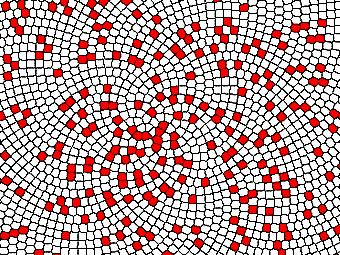
\includegraphics[width=0.95\columnwidth]{img/10.8 img1.jpg}
\end{minipage}
    \hfill
\begin{minipage}{0.5\linewidth}
    \footnotesize{\textit{''О, святая простота!'' - воскликнул Ян Гус, увидев старушку, несшую на его костер последнюю вязанку хвороста. Она была уверена, что делает благое дело, ради которого можно было и без хвороста померзнуть.}}
    \par
    \bigskip
    \normalsize{Для начала суммируем факты, доказанные в первой части и ранее.}
\end{minipage}
\end{figure}

\begin{state} \label{10.8 state1}
    Если $b | (ca)$ и НОД($a,~b$) = 1, то $b | c$.
\end{state}

\begin{dok}
    Воспользуемся теоремой из части 1. Поскольку НОД($a,~b$) = 1, то найдутся целые числа $u$ и $v$, такие, что $au + bv = 1$. Умножим обе части полученного равенства на $c$. Получим $acu + bcv = c$. Тогда первое слагаемое делится на $b$ потому что по условию $ac$ делится на $b$. Второе слагаемое также делится на $b$. Значит, и сумма, равная $c$, тоже делится на $b$.
\end{dok}

\begin{state} \label{10.8 state2}
    Любое общее кратное чисел $a$ и $b$ делится на НОК($a,~b$). \textit{(т.е. если $A$ делится на $a$ и $A$ делится на $b$, то $A$ делится на НОК($a$, $b$.)}
\end{state}

\begin{dok}
    От противного. Пусть существует кратное $K$, не делящееся на НОК($a,~b$) = $k$. Тогда $К = kn + r$, где $k > r > 0$. И $r$ делится на $a$ и $b$, т.е. также является общим кратным, но $r < k$ = НОК. Противоречие. 
\end{dok}

\begin{state}
    Любой общий делитель чисел $a$ и $b$ является делителем НОД($a,~b$)
\end{state}

\begin{state}
    Для любых целых чисел $a$ и $b$ НОД($a,~b$) = НОД($a,~a - b$).\footnotemark 
\end{state}\footnotetext{Напомним доказательство этого факта. Очевидно, что все общие делители чисел $a$ и $b$ являются делителями числа $a - b$. Аналогично, все общие делители чисел $a$ и $a - b$ являются делителями $b$. Следовательно, множества общих делителей чисел $a$ и $b$ и чисел $a$ и $a - b$ совпадают, поэтому совпадают и их наибольшие общие делители. Утверждение доказано.}

\begin{state}
    Если НОК($a,~b$) = $k$ и $m$ -- натуральное число, то НОК($am,~bm$) = $km$.
\end{state}

\begin{state}
    Если НОК($a,~b$) = $k$ и НОД($a,~b$) = $d$, то ($\dfrac{a}{d},~\dfrac{b}{d}$) = $\dfrac{k}{d}$.
\end{state}

\begin{state}
    Для любых натуральных чисел $a$ и $b$ справедливо $ab = НОД(a,~b) \times НОК(a,~b)$. В частности, для взаимно простых чисел $ab = НОК(a,~b)$.
\end{state}

\textbf{\textit{Доказательство факта: $ab = НОД(a,~b) \times НОК(a,~b)$.}}

\begin{enumerate}[itemsep=0.05em]
    \item Пусть $НОК(a,~b) = k$. Т.к. $ab$ является общим кратным для $a$ и $b$, то $ab = сk$ (см. утверждение \ref{10.8 state2}). Докажем, что $c = НОД(a,~b)$. Т.к. $k$ -- общее кратное, то $k M a$. Следовательно $k = am$ и $ab = сam \Rightarrow b = cm$, т.е. $c$ является делителем $b$. Аналогично, $c$ является делителем $a$. Значит, $c$ -- общий делитель $a$ и $b \Rightarrow НОД(a, b) \geq с \Rightarrow k = \dfrac{ab}{c} \geq \dfrac{ab}{d}$.
    
    \item Пусть НОД($a,~b$) = $d$ и $a$ = $a_1d,~b = b_1d$. Тогда $a_1b_1d = \dfrac{ab}{d}$ является общим кратным для $a$ и $b$. Следовательно, $\dfrac{ab}{d} \geq k = НОК(a,~b)$.
    
    \item Таким образом, из $1. \Rightarrow  k \geq \dfrac{ab}{d}$, а из $2. \Rightarrow \dfrac{ab}{d} \geq k$. Поэтому $\dfrac{ab}{d} = k$ и утверждение доказано. \hfill \qedsymbol
\end{enumerate}

\newpage

\textbf{\textit{Доказательство факта: если $ab$ делится на простое $p$, то либо $a$ делится на $p$, либо $b$ делится на $p$.}}

\begin{enumerate}[itemsep=0.05em]
    \item Если $p$ -- простое число, то любое другое натуральное число либо взаимно просто с $p$, либо делится на $p$. (Утверждение \ref{10.8 state1}.)

    \item Если $a$ и $p$ взаимно просты. Тогда $ap = НОК(a,~p)$. Известно, что $ab$ делится на $p$, но $ab$ делится и на $a$, но тогда $ab$ делится и на $НОК(a,~p)$, т.е. на $ap$. Следовательно, $ab = map$ и $b = mp$, т.е. $b$ делится на $p$. \hfill \qedsymbol
\end{enumerate}

\begin{dfn}
    Натуральное число $a$ называется простым, если оно имеет ровно два различных натуральных делителя и составным -- если больше двух. Число 1 не считается ни простым, ни составным.
\end{dfn}

\noindent Простые числа по определению не разлагаются в произведение меньших чисел. Почти очевидно следующее:

\begin{dfn}
    Каждое натуральное число большее 1 можно разложить в произведение простых.
\end{dfn}

\noindent Действительно, пусть нам дано составное число $a$. Мы можем разложить его в произведение двух множителей, меньших $a$. Если среди них есть хотя бы один не простой, то мы можем и его разложить в произведение двух множителей. Если среди них опять будут составные, они вновь разлагаются на множители и т.д. Этот процесс не может продолжаться бесконечно, поскольку каждый сомножитель меньше самого числа. В результате мы придём к разложению на простые множители. Обычно равные простые множители собирают вместе и записывают разложение так: $48 = 2^4 \times 3$. В общем случае: $a = p_1^{k_1} \times p_2^{k_2} \times ... \times p_m^{k_m}$, где $p_1, p_2, ..., p_m$ -- различные простые числа. Позже мы докажем, почему такое разложение единственно.
Чтобы начать процесс разложения данного числа $a$ в произведение простых, нужно найти хотя бы один простой множитель. Никакого простого способа для этого не существует: если про $a$ заранее ничего не известно, приходится перебирать простые числа и по очереди испытывать, делится ли $a$ на 2, 3, 5 и т.д. (В частности, один из способов поиска простых чисел был предложен Эратосфеном (\textit{решето Эратосфена}))

\begin{center}
  \fbox{\begin{varwidth}{0.95\textwidth}
    \begin{thrm} 
        \textit{(«Основная теорема арифметики»)} Каждое натуральное число разлагается на простые множители единственным образом.
    \end{thrm}
    \end{varwidth}}  
\end{center}

\begin{dok}
    Докажем сначала вспомогательную лемму: если числа $q, p_1, p_2, ..., p_n$ -- простые и произведение $p_1 \times р_2 \times ... \times p_n$ делится на $q$, то одно из чисел $p_i$ равно $q$. Для любого числа $p_i$ либо $p_i$ делится на $q$, либо $p_i$ и $q$ взаимно просты. Тогда для любых двух простых чисел справедливо одно из двух: либо они совпадают, либо взаимно просты. Будем доказывать лемму индукцией по количеству простых чисел $n$. 
    \\
    \textbf{База индукции:} $n = 2$. Пусть произведение $p_1 \times p_2$ делится на $q$. Если $p_1$ делится на $q$, то $p_1$ совпадает с $q$ и утверждение леммы доказано. Пусть $p_1$ не делится на $q$, тогда они взаимно просты и по утверждению \ref{10.8 state1} $p_2$ делится на $q$ и, следовательно, $p_2$ совпадает с $q$. База доказана. Пусть доказано для любого произведения $k$ простых чисел. Рассмотрим произведение $k + 1$ числа. Обозначим произведение первых $k$ чисел через $A = p_1 \times p_2 \times ... \times p_k$, тогда рассматриваемое произведение равно $p_1 \times p_2 \times ... \times p_k \times p_{k + 1} = A \times p_{k + 1}$. По условию оно делится на $q$. Если $p_{k + 1}$ делится на $q$, то $p_{k + 1}$ совпадает с $q$ и всё доказано. Если же не делится, то $p_{k + 1}$ и $q$ взаимно просты и, следовательно, $A$ делится на $q$ и мы получаем условие индукционного предположения. Тем самым переход доказан и лемма доказана.
\end{dok}

\begin{figure}[H]
\begin{minipage}{0.7\linewidth}
    Обобщая все доказанное, имеем: если $p_1, p_2, ..., p_n$ -- различные простые числа, а $a_2, a_3, ..., a_n$ -- неотрицательные целые числа. Тогда число $p_2^{a_2} \times p_3^{a_3} \times ... \times p_n^{a_n}$ не делится на $p_1$.
    \\
    Докажем теперь основную теорему арифметики. Понятно, что хотя бы одно разложение на простые множители существует. Докажем, что оно единственно с точностью до порядка сомножителей. От противного. Предположим, такое разложение не единственно. Рассмотрим два различных разложения для некоторого числа:  
    \begin{center}
       $A = p_1^{a_1} \times p_2^{a_2} \times ... \times p_n^{a_n} = q_1^{\beta_1} \times q_2^{\beta_2} \times ... \times q_k^{\beta_k}$. 
    \end{center}
    Сократив все одинаковые множители, получаем $p_1^{a_1} \times p_2^{a_2} \times ... \times p_n^{a_n} = q_1^{\beta_1} \times q_2^{\beta_2} \times ... \times q_k^{\beta_k}$, где все $p_i$ и $q_j$ различны. Но это противоречит доказанной выше лемме, согласно которой если $p_1^{a_1} \times p_2^{a_2} \times ... \times p_n^{a_n}$ делится на $q_1$, то один из множителей совпадает с $q_1$. Следовательно, среди чисел $p_i$ есть хотя бы одно, совпадающее с $q_1$. Получили противоречие с тем, что все $p_i$ и $q_j$ различны. Тем самым теорема доказана.
\end{minipage}
    \hfill
\begin{minipage}{0.29\linewidth}
    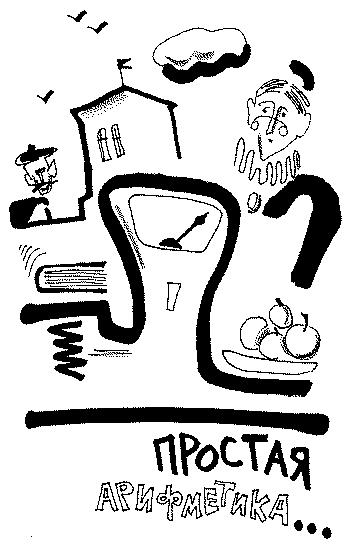
\includegraphics[width=0.95\columnwidth]{img/10.8 img2.png}
\end{minipage}
\end{figure}

\begin{ex}
    Пользуясь основной теоремой арифметики, выпишите общий вид НОД и НОК двух целых чисел.
\end{ex}

\begin{thm} $^{**}$
    Докажите, что если первый член и разность арифметической прогрессии взаимно просты, то среди её членов содержится бесконечно много простых чисел.
\end{thm}

\begin{thm}
    Докажите, что не существует такого многочлена $f(x) = a_0 x^n + a_1 x^{n - 1} + ... + a_{n - 1} x + a_n$ с целыми
коэффициентами, что все числа $f(0), f(1), f(2), f(3), ...$ являются простыми.
\end{thm}

\begin{thm}
    Пусть $p$ -- простое. Докажите, что тогда либо $a$ делится на $p$, либо что НОД($a$, $p$) = 1.
\end{thm}
\head{Апрель}{Листок 11. Делимость целых чисел -- 2.}

\section{Часть 3 -- "Евклидовая".}

\begin{center}
    \footnotesize{\textit{В задачах этого листка речь идёт только о целых числах.}}
\end{center}

\begin{center}
    \textit{\textbf{Лирическое отступление.}}
\end{center}

\begin{center}
  \fbox{\begin{varwidth}{0.95\textwidth}
      \begin{center}
          \textbf{Теорема Дирихле} \textit{(«о простых числах в арифметической прогрессии»)}
      \end{center}
    Каждое арифметическая прогрессия, первый член и разность которой -- натуральные, взаимно
    простые числа, содержит бесконечное число простых чисел.
    \end{varwidth}}  
\end{center}

Теорема Дирихле доказывается весьма сложно, и мы  в курсе её доказывать не будем. В 1950 году датский математик А. Сельберг придумал чрезвычайно сложное и хитроумное элементарное (не использующее аппарат высшей математики) доказательство теоремы Дирихле, однако жить лучше от этого не стало и даже сильно одарённому школьнику. Для желающих поломать голову добавим только, что по сути Дирихле доказал, что при любых фиксированных взаимно простых числах $m$ и $k$ $\underset{s \rightarrow 1+}{\textrm{lim}} \dfrac{ \underset{p}{\sum} \times \dfrac{1}{p^s}}{\textrm{ln} \frac{1}{s - 1}} = \dfrac{1}{\phi(k)}$, где суммирование ведётся по всем простым числам $p$ таким, что $p \equiv m~(\textrm{mod}~k)$, а $\phi (k)$ –- функция Эйлера. Это соотношение можно также интерпретировать как закон равномерного распределения простых чисел по классам вычетов по модулю $k$, так как при суммировании по всем простым числам $\underset{s \rightarrow 1+}{\textrm{lim}} \dfrac{ \underset{p}{\sum} \times \dfrac{1}{p^s}}{\textrm{ln} \frac{1}{s - 1}} = 1$. В качестве следствия из теоремы Дирихле можно также рассматривать утверждение, что ряд, составленный из обратных величин к простым числам из арифметической прогрессии, расходится. Красивым следствием из теоремы Дирихле является

\begin{center}
\fbox{\begin{varwidth}{0.95\textwidth}
    \begin{state}
        Не существует такого многочлена $f(x) = a_0 x^n + a_1 x^{n - 1} + ... + a_{n - 1}x + a_n$~с целыми коэффициентами такими, что все числа $f(0), f(1), f(2), f(3), ...$ являются простыми.
    \end{state}
    \end{varwidth}}
\end{center}

Впервые несложное доказательство этого факта придумал сам Эйлер. Он же напридумывал массу многочленов $f(x)$, значения которых при многих последовательных натуральных $x$ являются простыми числами. Например:

\begin{enumerate}[noitemsep, label=\asbuk*), ref=\asbuk*]
    \item $f(x) = x^2 + x + 41$, при $x = 0, 1, 2, ..., 39$.
    \item $f(x) = x^2 - 79x + 1601$, при $x = 0, 1, 2, ..., 79$.
\end{enumerate}

С первым многочленом вы должны быть хорошо знакомы -- мы рассматривали его в листке «Индукция», когда говорили о догадках по аналогии. Интересно, что если же рассматривать многочлены от нескольких переменных, то многочлены, множество положительных значений которых в точности является множеством всех простых чисел, существуют.\footnote{Этот факт был доказан Юрием Матиясевичем в 1970 году.} Нам удалось разыскать один из таких многочленов от 26 переменных, который и приводим здесь \smiley:

\begin{center}
$P(a, b, c, d, e, f, g, h, i, j, k, l, m, n, o, p, q, r, s, t, u, v, w, x, y, z) = \{k + 2\}\{1 - (wz + h + j – q)^2 - (2n + p + q + z – e)^2 – (a^2y^2 – y^2 + 1 – x^2)^2 – (\{e^4 + 2e^3\}\{a + 1\}^2 – o^2)^2 – (16\{k + 1\}^3\{k + 2\}\{n + 1\}^2 + 1 – f^2)^2 – (\{(a + u^4 – u^2a)^2 – 1\}\{n + 4dy\}^2 + 1 – \{x + cu\}^2)^2 – (ai + k + 1 – l – i)^2 – (\{gk + 2g + k + 1\}\{h + j\} + h – z)^2 – (16r^2y^4\{a^2 – 1\} + 1 - u^2)^2 – (p – m + l\{a – n – 1\} + b\{2an + 2a – n^2 – 2n – 2\})^2 – (z - pm + pla – p^2l + t\{2ap – p^2 – 1\})^2 – (q – x + y\{a – p – 1\} + s\{2ap + 2a – p^2 – 2p – 2\})^2 – (a^2l^2 – l^2 + 1 – m^2)^2 – (n + l + v – y)^2\}$
\end{center}

\section{Решение уравнений в целых числах.}

Отдельным большим разделом математики является область, посвящённая решению уравнений в целых числах. Эта математическая задача является одной из древнейших. Апогея своего расцвета эта область математики достигла в Древней Греции. Наиболее известным источником, дошедшим до нашего времени, является произведение Диофанта –- «Арифметика». Диофант суммировал и расширил накопленный до него опыт решения неопределённых уравнений в целых числах. И до сих пор целочисленные уравнения называются \textit{диофантовыми}.
\par
История сохранила нам мало черт биографии замечательного александрийского учёного-алгебраиста. По некоторым данным Диофант жил до 364 года н.э. Достоверно известно лишь своеобразное жизнеописание учёного, которое по преданию было высечено на его надгробии и представляло задачу-головоломку:

\textit{«Бог ниспослал ему быть мальчиком шестую часть жизни; добавив к сему двенадцатую часть, Он покрыл его щеки пушком; после седьмой части Он зажёг ему свет супружества и через пять лет после вступления в брак даровал ему сына. Увы! Несчастный поздний ребёнок, достигнув меры половины полной жизни отца, он был унесён безжалостным роком. Через четыре года, утешая постигшее его горе наукой о числах, он (Диофант) завершил свою жизнь» (попробуйте решить задачу самостоятельно).}

\begin{ex}
    Пусть $ax = by$ и НОД($a$, $b$) = 1. Докажите, что тогда найдётся такое число $t$, что $x = bt, y = at$.
\end{ex}

\begin{ex}
    Пусть $ax = by$ и НОД($a$, $b$) = 1. Опишите все пары целых чисел ($x$, $y$), являющиеся решениями данного уравнения.
\end{ex}

\begin{ex}
    Найдите все целые решения уравнения $12x + 14y = 0$.
\end{ex}

\begin{figure}[H]
\begin{minipage}{0.6\linewidth}
    Пусть на клетчатой бумаге нарисован прямоугольник размером $a \times b$ клеток (стороны прямоугольника идут по линии сетки). Проведём диагональ и отметим все узлы сетки, которые на ней лежат. На сколько частей эти узлы делят диагональ? (Узлами мы называем точки, где пересекаются линии сетки.)
    \begin{enumerate}[noitemsep, label=\asbuk*), ref=\asbuk*]
    \item  Решите задачу для прямоугольника размером 10$\times$15. (см. рис.)
    \item  Решите задачу в общем виде.
    \end{enumerate}
    \end{minipage}
    \hfill
\begin{minipage}{0.39\linewidth}
    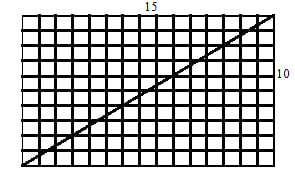
\includegraphics[width=0.95\columnwidth]{img/11.2 img1.jpg}
\end{minipage}
\end{figure}

Рассмотрим уравнение $ax + by = c$, где $a$, $b$ и $c$ -- целые числа. Наша задача -- определить, при каких условиях это уравнение имеет решение в целых числах $x$ и $y$, и какой вид имеют эти решения.

\begin{thm}
    Докажите, что уравнение $ax + by = c$ имеет решение в целых числах тогда и только тогда, когда $c$ делится на $d$ = НОД ($a$, $b$).
\end{thm}

\begin{thm}
    Докажите, что если НОД($a$, $b$) = 1, то уравнение $ax + by = c$ имеет бесконечное множество решений.
\end{thm}

\begin{thm} \ref{11.2 thm1}
    Докажите, что если пара чисел ($x_0$, $y_0$) -- решение уравнения $ax + by = c$, то все решения имеют вид $x = x_0 - bt$, $y = y_0 + at$, где $t$ -- любое целое число
\end{thm}

\textit{\underline{Замечание.}} Когда решение уравнения приводится в виде, зависящем от некоторого параметра, говорят, что приведено общее решение уравнения. Какое--нибудь конкретное значение чисел $x$ и $y$ называется частным решением исходного уравнения. Таким образом, ($x_0$, $y_0$) -- частное решение уравнения, а $x = x_0 - bt$, $y = y_0 + at$ -- общее решение исходного уравнения.

\begin{ex}
    Какие из приведённых ниже наборов чисел являются для уравнения $12x - 15y = 6$
    \par 
    1) решениями; 2) частными решениями; 3) общими решениями.
    \begin{enumerate}[noitemsep, label=\asbuk*), ref=\asbuk*]
        \item $x = -2$,~$y = -2$; 
        \item $x = 3 + 15t,~y = 2 + 12t$, где $t$ -- любое целое число;
        \item $x = -2 + 5t, y = -2 + 4t$, где $t$ -- любое
        целое число;
        \item $x = 15t, y = 12t$, где $t$ -- любое целое число; 
        \item $x = 3 + 5t, y = 2 + 4t$, где $t$ -- любое целое число.
    \end{enumerate}
\end{ex}

\begin{thm}
    Докажите, что если c делится на $d$ = НОД($a$, $b$) и $a$ = $a_1d$, $b = b_1d$, $c = c_1d$, то числа ($x_0$, $y_0$) одновременно являются или не являются решениями уравнений $ay - bx = c$ и $a_1y - b_1x = c_1$.
\end{thm}

\begin{thm}
    Имеют ли следующие уравнения решения в целых числах: 
    \par а) $6x - 16y = 220$; б) $105x + 42y = 56$?
\end{thm}

\begin{center}
    \textbf{Алгоритм Евклида.}\footnote{Евклид -- древнегреческий математик, автор первого из дошедших до нас теоретических трактатов по математике.}
\end{center}

\begin{figure}[H]
\begin{minipage}{0.15\linewidth}
    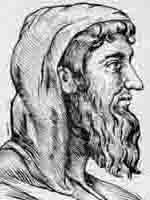
\includegraphics[width=0.95\columnwidth]{img/11.2 img2.jpg}
\end{minipage}
\hfill
\begin{minipage}{0.85\linewidth}
    Слово «алгоритм» означает «общий метод, применимый к целому классу задач». Обычно в математике подразумевается, что этот метод можно сформулировать в виде совершенно точного описания -- настолько точно и определенно, что любой человек, умеющий только читать и считать, может его выполнить (для любой конкретной задачи, т.е. для любых заданных ему значений параметров).
    \\
    \textit{Алгоритм Евклида} -- это правило, которое позволяет по двум натуральным числам $a$ и $b$ найти НОД($a$, $b$).
\end{minipage}
\end{figure}

Например, для нахождения наибольшего общего делителя двух чисел подходит и такой алгоритм:
\begin{enumerate}[noitemsep]
    \item найти все делители числа $a$ (перепробовать все числа: 1, 2, ..., не превосходящие $a$);
    \item найти все делители чисел $a$ и $b$ (проверив, на какие из делителей $a$ делится $b$);
    \item выбрать из общих делителей наибольший.
\end{enumerate}

\begin{figure}[H]
\begin{minipage}{0.74\linewidth}
    Конечно, если числа достаточно малы, то проще найти НОД, отыскав все делители обоих чисел или разложив оба числа на простые множители. А если числа очень велики и даже разложение на простые множители является проблематичным? Алгоритм Евклида позволяет найти НОД($a$, $b$) в этих случаях значительно быстрее, не отыскивая всех делителей ни у одного из чисел $a$ и $b$. Он основан на следующих фактах.
    \begin{thm}
        Докажите утверждение 4 из части 2, т.е. докажите, что НОД($b$, $a$ - $b$) = НОД($a$, $b$).
    \end{thm}
    \begin{thm}
        Пусть $a = bq + r$. Докажите, что тогда НОД($b$, $r$) = НОД($a$, $b$).
    \end{thm}
    Это утверждение позволяет легко и быстро находить НОД двух чисел.
    \\
    Покажем, как это делается.

% здесь нужно вставить таблицу
% \begin{table}[h]
% \begin{tabular}{ll}
%     $1014 = 2733 \times 3 + 195$ \hfill 
%     \\
%     $273 = 195 \times 1 + 78$ \hfill = 
%     \\
%     $195 = 78 \times 2 + 39$ \hfill = 
%     \\
%     $78 = 39 \times 2$ \hfill = 
%  & 
%      НОД(273, 1014) =
%     \\
%     НОД(195, 273) =
%     \\
%     НОД(195, 78) =
%     \\
%     НОД(78, 39) = 39
% \end{tabular}
% \end{table}
{
\begin{tabular}{ll}
$1014 = 2733 \times 3 + 195$ & НОД(273, 1014) = \\
$273 = 195 \times 1 + 78$ & = НОД(195, 273) = \\
$195 = 78 \times 2 + 39$ & = НОД(195, 78) = \\
$78 = 39 \times 2$ & = НОД(78, 39) = 39 \\
\end{tabular}
}

    \noindent \underline{Ответ:} НОД(273, 1014) = 39. \hfill \qedsymbol
\\
Приведённый выше метод отыскания наибольшего делителя и носит название \textit{алгоритма Евклида.}

Алгоритм Евклида в общем случае можно описать так: если имеются два целых числа $a$ и $b$, причем $a$ > $b$ > 0, то сначала делим $a$ на $b$, и получаем остаток $r_1$, который меньше, чем $b$. Затем делим число $b$ на $r_1$, находим остаток $r_2$, который меньше, чем $r_1$. Далее мы делим число $r_1$ на $r_2$, при этом получим остаток $r_3$, меньший, чем $r_2$ и так далее, пока какой-нибудь остаток $r_{n – 1}$ не разделится на остаток $r_n$ нацело, без остатка (т.е. $r_{n + 1} = 0$). Ясно, что указанный процесс обязательно кончится, поскольку каждый остаток меньше предыдущего, а все остатки -- неотрицательные числа. Последний остаток и есть НОД($a$, $b$). Действительно: 
\\
$r_n = НОД(r_n, r_{n - 1}) = НОД(r_{n - 1}, r_{n - 2}) = НОД(r_{n - 2}, r_{n - 3}) = ... = НОД(r_2, r_1) = НОД(r_1, b) = НОД(a, b)$.
\end{minipage}
\begin{minipage}{0.25\linewidth}
    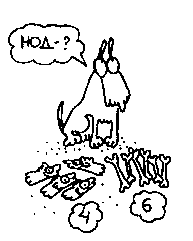
\includegraphics[width=0.95\columnwidth]{img/11.2 img3.png}
    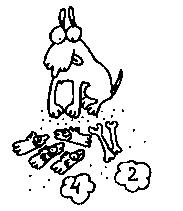
\includegraphics[width=0.95\columnwidth]{img/11.2 img4.png}
    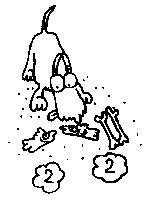
\includegraphics[width=0.95\columnwidth]{img/11.2 img5.png}
\end{minipage}
\end{figure}

\noindent \textbf{\textit{Пример.}} Найти НОД(273, 1014).

\textit{\textbf{Решение.}} Выполняем деление с остатком:
% \begin{figure}[H]
% \begin{minipage}{0.3\linewidth}
    % $1014 = 2733 \times 3 + 195$ \hfill 
    % \\
    % $273 = 195 \times 1 + 78$ \hfill = 
    % \\
    % $195 = 78 \times 2 + 39$ \hfill = 
    % \\
    % $78 = 39 \times 2$ \hfill = 
% \end{minipage}
% \begin{minipage}{0.3\linewidth}
    % НОД(273, 1014) =
    % \\
    % НОД(195, 273) =
    % \\
    % НОД(195, 78) =
    % \\
    % НОД(78, 39) = 39
% \end{minipage}
% \hfill
% \begin{minipage}{0.25\linewidth}
%     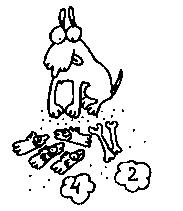
\includegraphics[width=0.95\columnwidth]{img/11.2 img4.png}
% \end{minipage}
% \end{figure}


\begin{ex}
    Найдите наибольший делитель чисел:
    \\
    а) 987654321 и 123456789; \hfill б) 16484 и 42282; \hfill в) 7777777777 и 777777.
\end{ex}

Покажем теперь, как алгоритм Евклида позволяет найти решение уравнения в целых числах. Согласно задаче \label{11.2 thm1} достаточно найти только какое--нибудь частное решение исходного уравнения, после чего общее решение тут же выписывается. Конечно, можно просто угадать, если же угадать сложно, то в нахождении такого решения как раз и поможет алгоритм Евклида. Если нужно решить уравнение $ax - by = c$ (можно считать, что $b$ > 0), отыскиваем с помощью алгоритма Евклида НОД($a$, $b$)

\begin{figure}[H]
    \centering
        \begin{minipage}{0.3\linewidth}
            $a = bq_0 + r_1;$
            \\
            $b = r_1q_1 + r_2;$
            \\
            $r_1 = r_2q_2 + r_3;$
            \\
            $...$
            \\
            $r_{n - 2} = r_{n - 1}q_{n - 1} + r_n;$
            \\
            $r_{n - 1} = r_nq_n$
        \end{minipage}
        \begin{minipage}{0.5\linewidth}
            $d = r_n$
            \\
            Теперь, возвращаясь по цепочке вверх, выписываем
            \\
            представление для $d$ через $a$ и $b$ в виде $a_{x_0} - b_{y_0}$.
            \\
            Найденные целые числа $x_0$ и $y_0$ и есть искомое
            \\
            частное решение исходного уравнения.
            \\

        \end{minipage}
\end{figure}

\begin{thm}
    Найдите решение уравнений в целых числах:
    \par а) 75y - 39x = 1; б) 43x + 250y = 7.
\end{thm}

\begin{thm}
    а) Костя живет в стандартном четырнадцатиэтажном доме в квартире 270. На каком этаже может располагаться его квартира? (На лестничной площадке одно и то же число квартир) 
    \par б)* Вообще, как быстро определить, может ли квартира с данным номером находиться на данном этаже?
\end{thm}

\begin{ques}
    Какая похожая задача была у нас в листке 5 про делимость?
\end{ques}
\section{Часть 4 -- "Цепная".}

\section{Цепные дроби.}

Вернёмся к алгоритму Евклида и посмотрим, что происходит с дробью $\dfrac{a}{b}$ в процессе нахождения наибольшего общего делителя.


$\dfrac{a}{b} = \dfrac{bq_0 + r_1}{b} = q_0 + \cfrac{r_1}{b} = q_0 + \cfrac{1}{\cfrac{b}{r_1}} = q_0+\cfrac{1}{\cfrac{r_1q_1 + r_2}{r_1}} = q_0 + \cfrac{1}{q_1 + \cfrac{1}{\cfrac{r_1}{r_2}}} = \cdots = q_0 + \cfrac{1}{q_1 + \cfrac{1}{q_2 + \cfrac{1}{q_3 + \cdots \cfrac{1}{q_{n - 1} + \cfrac{1}{q_n}}}}}$

\noindent Представление дроби $\dfrac{a}{b}$ в таком виде называется \textit{цепной дробью}.

\underline{\textit{Обозначение:}} $\dfrac{a}{b} = [q_0; q_1, q_2, \cdots, q_n]$ -- если дробь конечна и $\dfrac{a}{b} = [q_0; q_1, q_2 , \cdots]$ -- если дробь бесконечна.

\begin{dfn} 
    \textit{Цепная дробь} (или \textit{непрерывная}) -- это математическое выражение вида $[q_0; q_1, q_2, \cdots] = q_0 + \cfrac{1}{q_1 + \cfrac{1}{q_2 + \cfrac{1}{q_3 + \cdots}}}$, где $q_0$ -- целое число, а остальные $q_i$ -- натуральные. 
\end{dfn} 

\noindent Очевидно, что таким образом можно представить любое действительное число можно представить цепной дробью (конечной или бесконечной).

\begin{thm}
    Докажите, что число представляется конечной цепной дробью тогда и только тогда, когда это число рационально.
\end{thm}

\noindent Если в какой-то момент «оборвать» непрерывную дробь, то можно получить конечную дробь, после преобразований сводящуюся к обыкновенной дроби. Такие дроби называются \textit{подходящими}.

Например, $2 + \cfrac{1}{3 + \dfrac{1}{4}} \left(= \dfrac{30}{13} \right), 5 + \cfrac{1}{1 + \cfrac{1}{3 + \dfrac{1}{2}}} \left(= \dfrac{52}{9}\right).$

Введём обозначения: 
\par $\dfrac{q_0}{1} = \dfrac{P_0}{Q_0}; q_0 + \dfrac{1}{q_1} = \dfrac{P_0}{Q_0}; q_0 + \cfrac{1}{q_1 + \dfrac{1}{q_2}} = \dfrac{P_2}{Q_2}; \cdots q_0 + \cfrac{1}{q_1 + \cfrac{1}{q_2 + \cfrac{1}{{ \substack{q_3 + \cdots\\[1pt]\cdots \cfrac{1}{q_n}}  }} } } = \dfrac{P_n}{Q_n}; \cdots$

\begin{figure}[H]
    \begin{minipage}{0.8\linewidth}
        \begin{thm}
            Представьте число $\dfrac{987}{654}$ виде цепной дроби.
        \end{thm}
        
        \begin{thm}
            Выразите отношение сторон прямоугольного поля, разбитого на квадратные участки (план изображён на рисунке), через цепную дробь.
        \end{thm}
        
        \begin{thm}
            Выразите $\dfrac{P_k}{Q_k} - \dfrac{P_{k - 1}}{Q_{k - 1}}$ и $\dfrac{P_k}{Q_k} - \dfrac{P_{k - 2}}{Q_{k - 2}}$ через $q_0, q_1, \cdots, q_n$. 
        \end{thm}
    \end{minipage}
\hfill
    \begin{minipage}{0.19\linewidth}
        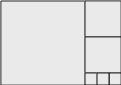
\includegraphics[width=0.95\columnwidth]{img/11.3 img1.png}
    \end{minipage}
\end{figure}

\begin{center}
    \fbox{\begin{varwidth}{\linewidth}
            \begin{thrm}
                («Свойство вилки»).
                \begin{center}
                      $\dfrac{P_1}{Q_1} > \dfrac{P_3}{Q_3} > \cdots > \dfrac{P_{2i - 1}}{Q_{2i - 1}} > \cdots$
                      \par
                      $\dfrac{P_0}{Q_0} < \dfrac{P_2}{Q_2} < \cdots < \dfrac{P_{2k}}{Q_{2k}} < \cdots$
                      \par
                      $\dfrac{P_{2i - 1}}{Q_{2i - 1}} > \dfrac{P_{2k}}{Q_{2k}} (i = 1, 2, \cdots; k = 0, 1, \cdots)$
                  \end{center}
            \end{thrm}
        \end{varwidth}}    
\end{center}


\begin{center}
    \textbf{Замечания к алгоритму Евклида для программистов или что такое алгоритм.}\footnote{День программиста – неофициальный праздник, отмечаемый на 256-й день года. \smiley}
\end{center}

\begin{figure}[H]
    \begin{minipage}{0.65\linewidth}
        Алгоритм Евклида часто (особенно в программировании) называют методом вычитаний. Почему так? По сути, выполняя деление с остатком, мы несколько раз вычитаем делитель, пока результат не станет меньше этого делителя. НОД при этом сохраняется. Попробуем алгоритмизировать приведенный выше пример нахождения НОД (273, 1014).
    \end{minipage}
\hfill
    \begin{minipage}{0.29\linewidth}
        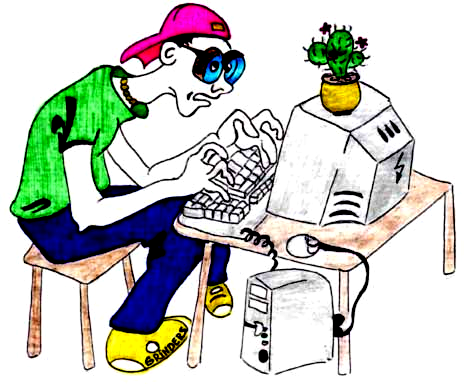
\includegraphics[width=0.95\columnwidth]{img/11.3 img2.png}
    \end{minipage}
\end{figure}


\begin{center}
    \begin{tabularx}{\textwidth} { 
  | >{\centering\arraybackslash}X 
  | >{\centering\arraybackslash}X 
  | >{\centering\arraybackslash}X 
  | >{\raggedright\arraybackslash}X | }
  \hline
   & \textit{математик} & \textit{программист} & \textit{находят} \\
  \hline
    1014 = 273 $\times$ 3 + 195 & делит 1014 на 273 с остатком & вычитает из 1014 число 273 три раза & НОД(273, 1014) \\
  \hline
    273 = 195 $\times$ 1 + 78 & делит 273 на 195 с остатком & вычитает из 273 число 195 & НОД(195, 273) \\
  \hline
    195 = 78 $\times$ 2 + 39 & делит 195 на 78 с остатком & вычитает из 195 число 78 два раза & НОД(195, 78) \\
  \hline
    78 = 39 $\times$ 2 & делит 78 на 39 без остатка & вычитает из 78 число 39 два раза & НОД(78, 39)  \\
  \hline
     & обнаруживает отсутствие остатка & получает ноль & НОД = 39 \\
  \hline
\end{tabularx} 
\end{center}

\noindent Мы продемонстрировали, как сформулировать алгоритм Евклида в виде, удобном для программирования. Очевидно, что гораздо проще запрограммировать действия столбца 3, а не 2, например, записав действие как «вычитать пока…». Когда в программировании употребляется слово «алгоритм», подразумевается, что все выполняемые операции определяются однозначно и для любых допустимых входных данных за конечное время порождается результат (выходные данные). В приведенном выше примере конечность алгоритма следует из уменьшения чисел на каждом шаге.

\begin{exP}
    Напишите программу, находящую НОД двух целых чисел. Заметим, что метод вычитаний эффективно работает и для любого количества целых числе, когда вручную найти НОД уже проблематично. Сформулируем этот метод для нескольких положительных чисел, а затем приведём его в виде, удобном для программирования. Итак, пусть дан набор целых положительных чисел, необходимо найти НОД всех этих чисел.
\end{exP}

\noindent \underline{\textit{Алгоритм:}} 

\begin{enumerate}[label=\arabic*), noitemsep] 
    \item Выберем из набора два различных положительных числа. (если они все равны одному и тому же числу, то НОД уже найден -- это и есть это число)
    \item Вычтем из большего меньшее.
    \item Если ещё есть различные числа, то перейдём к пункту 1), если нет -- НОД найден.
\end{enumerate}

\newpage

Ниже в таблице приведён пошаговый пример программной реализации метода вычитания. При этом вместо выбора двух различных положительных чисел используется «выбор двух случайных положительных числа набора», что возможно благодаря наличию датчиков псевдослучайных чисел в программном обеспечении компьютера.

\begin{center}
    \begin{tabularx}{\textwidth}{ |c|c|c|c|c|c|X| }
\hline
    \textit{номер шага} & \textit{1-е число} & \textit{2-е число} & \textit{3-е число} & \textit{4-е число} & \textit{сумма чисел} & \textit{что ищем} \\
\hline
    Шаг 1 & \textbf{72} & 84 & \textbf{132} & 144 & 432 & НОД(72; 84; 132; 144) \\
\hline
    Шаг 2 & \textbf{72} & \textbf{84} & 60 & 144 & 360 & НОД(72; 84; 60; 144) \\
\hline
    Шаг 3 & 72 & \textbf{12} & 60 & \textbf{144} & 288 & НОД(72; 12; 60; 144) \\
\hline
    Шаг 4 & 72 & 12 & \textbf{60} & \textbf{132} & 276 & НОД(72; 12; 60; 132) \\
\hline
    Шаг 5 & \textbf{72} & 12 & 60 & \textbf{72} & 216 & НОД(72; 12; 60; 72) \\
\hline
    Шаг 6 & \textbf{72} & 12 & \textbf{60} & 0 & 144 & НОД(72; 12; 60) \\
\hline
    Шаг 7 & \textbf{12} & \textbf{12} & 60 & 0 & 84 & НОД(12; 12; 60) \\
\hline
    Шаг 8 & \textbf{12} & 0 & \textbf{60} & 0 & 72 & НОД(12; 60) \\
\hline
    Шаг 9 & \textbf{12} & 0 & \textbf{48} & 0 & 60 & НОД(12; 48) \\
\hline
    Шаг 10 & \textbf{12} & 0 & \textbf{36} & 0 & 48 & НОД(12; 36) \\
\hline
    Шаг 11 & \textbf{12} & 0 & \textbf{24} & 0 & 36 & НОД(12; 24) \\
\hline
    Шаг 12 & \textbf{12} & 0 & \textbf{12} & 0 & 24 & НОД(12; 12) \\
\hline
    Шаг 13 & 12 & 0 & 0 & 0 & 12 & НОД = 12 \\
\hline
    \end{tabularx} 
\end{center}

Выбирая для вычитания различные пары, можно получить разные алгоритмы. Все эти алгоритмы будут решать поставленную задачу. Для того чтобы в этом убедиться, необходимо обосновать корректность алгоритмов, т.е. доказать, что каждый такой алгоритм обязательно закончит свою работу, что полученный в результате работы алгоритма набор будет содержать только одно ненулевое число и что это число будет наибольшим общим делителем исходного набора.

\fbox{\begin{varwidth}{\linewidth}
    \textbf{\textit{Обоснование корректности алгоритма}} -- очень важный этап как для программистов, так и для математиков.
\end{varwidth}}    

\noindent Доказать корректность изложенного метода несложно.

\begin{dok}
    \begin{enumerate}[noitemsep] 
        \item Для доказательства заметим, что НОД($a_1, a_2, ..., a_n$) = НОД($a_1, a_2, ..., a_i, ..., a_j - a_i, ..., a_n$).
            \begin{ex}
                Докажите этот факт.
            \end{ex}
            Следовательно, указанная операция над набором чисел сохраняет общие делители набора. Аналогично можно доказать, что эта операция не добавляет новых общих делителей. Мы доказали, что на каждом шаге алгоритма \textit{множество общих делителей не меняется}.
        \item Далее заметим, что при указанных преобразованиях \textit{числа набора остаются неотрицательными}. Действительно, вычитая из положительного числа меньшее (или равное ему), мы получим неотрицательное число. Поэтому операцию вычитания можно осуществлять до тех пор, пока в наборе есть хотя бы два положительных числа.
        \item Наконец, \textit{процесс изменения набора обязательно закончится}, т.к. после каждого вычитания сумма чисел набора уменьшается. В то же время эта сумма всегда есть положительное целое число, следовательно, процесс не может длиться бесконечно (очевидно, что число шагов не превышает суммы чисел исходного набора).
    \end{enumerate}
    
\end{dok}

\begin{exP}
    Напишите программу, находящую НОД $n$ целых чисел (число $n$ вводится и заранее неизвестно).
\end{exP}
\head{Апрель}{Листок 11. Делимость целых чисел -- 2. Уровень 1}

\section{В задачах этого листка речь идёт только о целых числах.}

\begin{thm}
     Выберите из следующих чисел все пары взаимно простых чисел: 10, 12, 17, 25, 44, 77, 68, 121.
\end{thm}

\begin{thm}
    Найдите: \textbf{а)} НОД(105; 77), НОК (105, 77); \textbf{б)} НОД(100!, 102!); НОК(100! + 101!; 101! + 102!)
\end{thm}

\begin{thm}
    При каких натуральных $n$ будут взаимно простыми числа: \textbf{а)} $10n + 1$ и $3n + 2$ \textbf{б)} $(n + 1)(n + 2)$ и $2n$?
\end{thm}

\begin{thm}
    При каких натуральных $n$ \textbf{а)} число $n + 13$ делится на $n + 3$; \textbf{б)} число $n^3 + 27$ делится на $7 - n$?
\end{thm}

\begin{thm}
    Верно ли, что, если НОД($a$, $b$) = НОД($b$, $c$) = $d$, то и НОД($a$, $c$) = $d$?
\end{thm}

\begin{thm}
    Докажите, что если НОД($a$, $b$) = $d$ и $a$ = $a_1d$, $b$ = $b_1d$, то числа $a_1$, $b_1$ взаимно простые.
\end{thm}

\begin{thm} $^n$
    Докажите, что любой общий делитель чисел $a$ и $b$ является делителем НОД($a$, $b$).
\end{thm}

\begin{thm}
    Докажите, что если НОК($a$, $b$) = $k$ и $m$ -- натуральное число, то НОК($am$, $bm$) = $km$.
\end{thm}

\begin{thm} $^n$
    Докажите, что если НОК($a$, $b$) = $k$ и НОД($a$, $b$) = $d$, то НОК $\left( \dfrac{a}{d}, \dfrac{b}{d} \right) = \dfrac{k}{d}$.
\end{thm}

\begin{thm}
    Докажите теорему \ref{11.0 thrm1} из теоретического листка: для любых натуральных чисел $a$ и $b$ справедливо $ab$ = НОД($a$, $b$) $\times$ НОК($a$, $b$).
\end{thm}

\begin{thm}
    Докажите, что если $b | (ca)$ и НОД($a$, $b$) = 1, то $b | c$.
\end{thm}

\begin{thrm}
    Пусть $ax = by$ и НОД($a$, $b$) = 1. Докажите, что тогда найдётся такое число $t$, что $x = bt$, $y = at$.
\end{thrm}
\head{Апрель}{Листок 11. Делимость целых чисел -- 2. Уровень 2}

\section{В задачах этого листка речь идёт только о целых числах.}

\begin{figure}[h]


    \begin{minipage}{0.25\linewidth}
        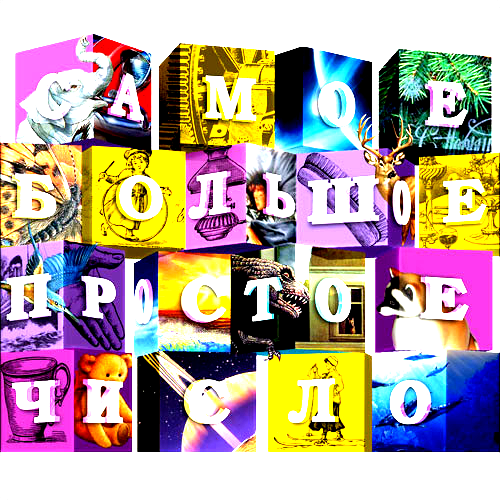
\includegraphics[width=0.95\columnwidth]{img/11.5 sbpch.png}
    \end{minipage}
    \hfill
    \begin{minipage}{0.73\linewidth}
\begin{thm}
    Пусть $p$ -- простое. Докажите, что тогда либо $a$ делится на $p$, либо НОД($a$, $p$) = 1.
\end{thm}

\begin{thm}
    \textbf{а)} Докажите, что если четырехзначное число $p$ не делится ни на одно простое число от 2 до 97, то $p$ -- простое. \textbf{б)} Докажите, что каждое составное число $a$ имеет простой делитель $p$ такой, что $p_2 \leq a$.
\end{thm}

\begin{thm}
    Докажите, что множество простых чисел бесконечно.
\end{thm}

\begin{thm}
    Известно, что $p$, $p$ + 10 и $p$ + 14 -- простые числа. Найдите $p$.
\end{thm}

        
    \end{minipage}

\end{figure}
    
\begin{thm} $^n$
    Известно, что $p$, $4p_2$ + 1 и $6p_2$ + 1 -- простые числа. Найдите $p$.
\end{thm}

\begin{thm}
    Известно, что $p$ и $p^2$ + 2 -- простые числа. Докажите, что $p^3$ + 2 также простое число.
\end{thm}

\begin{thm}
    Докажите, что если $(n - 1)! + 1$ делится на $n$, то $n$ -- простое число.
\end{thm}

\begin{thm}
    Докажите, что существует такое натуральное $n$, что числа $n + 1$, $n + 2$, ..., $n + 2013$ -- составные.
\end{thm}

\begin{thm}
    Пользуясь идеями двух предыдущих задач, докажите, что для любого $n$ существует $n$ подряд идущих составных чисел.
\end{thm}

\begin{thm}
    Докажите, что среди членов каждой из арифметических прогрессий:
    \par а) 3, 7, 11, 15, 19, ... \hfill б) 5, 11, 17, 23, 29, ... \hfill в) 11, 21, 31, 41, 51, ...
    \par имеется бесконечно много простых чисел.
\end{thm}
\head{Апрель}{Листок 12. Дополнительный. Системы счисления.}

«Из подъезда вышел человек лет около 49; пройдя по улице метров 196, он зашел в магазин, купил там две семёрки яиц и пошёл дальше...». Такое описание звучит несколько странно, не правда ли? Обычно, приблизительно оценивая какую--либо величину, мы пользуемся круглыми числами: «метров 200», «лет 50» и т.п. Говоря о круглых числах, мы обычно не отдаём себе отчёта в том, что деление чисел на круглые и некруглые по существу условно, и одно и то же число может быть круглым или некруглым в зависимости от того, какой системой счисления мы пользуемся.

Прежде разберёмся, что представляет собой наша десятичная система счисления, которой мы обычно пользуемся. Например, запись 2345 означает, что данное число содержит 5 единиц, 4 десятка, 3 сотни и 2 тысячи, т.е. 2345 -- сокращённое обозначение выражения

\begin{equation}
    2 \times 10^3 + 3 \times 10^2 + 4 \times 10^1 + 5 \times 10^0.
\end{equation}

Мы получили разложение по степеням числа 10. Как в первом классе, объясняя нам, что такое десятки, учительница предлагала связать в пучок 10 палочек и назвать этот пучок \textit{десятком}, связав десять таких пучков в больший пучок назвать последний \textit{сотней} и т.д. И запись нашего числа означает всего лишь сколько каких “пучков“ надо взять, чтобы получить рассматриваемое число. Однако с таким же успехом можно представить любое число в виде комбинации степеней не числа 10, а любого другого натурального числа (кроме 1), например, семи. В этой системе, называемой \textit{семеричной системой счисления} или \textit{системой счисления с основанием 7}, мы вели бы счёт от 0 до 6 обычным образом, а число 7 приняли бы за единицу следующего разряда. (Тогда бы в первом классе мы связывали бы пучки не по 10 палочек, а по семь.) Т.е. само число 7 в нашей семеричной системе счисления было бы обозначено символом 10. Чтобы не путать обозначения в разных системах счисления принято нижним индексом обозначать, в какой системе счисления мы работаем: 710 = 107.

\begin{thm}
    Верно ли, что для любого натурального числа $p > 1$ справедливо равенство $p_{10} = 10_р$?
\end{thm}

\begin{dfn} \label{11.6 dfn1}
    $\left( \overline{a_ka_{k-1}...a_1a_0} \right)_p = a_k \times p^k + a_{k - 1} \times p^{k - 1} + ... + a_1 \times p + a_0$, \hfill (*)
    \par где натуральные числа $a_i < p$.   
\end{dfn}

\noindent Заметим, что в $p$--ичной системе счисления круглыми будут совсем не те числа, которые были круглыми в десятичной системе. Например, в приведённом в самом начале все используемые в рассказе числа являются круглыми в семеричной системе счисления.

\begin{ex} $^*$
    Запишите числа в рассказе в семеричной системе счисления.
\end{ex} 

\noindent Системы счисления, о которых мы говорим, строятся по одному общему принципу. Выбирается некоторое число $p$ -- \textit{основание системы счисления}, и каждое число $N$ представляется в виде комбинации его степеней с коэффициентами, принимающими значения от 0 до $p - 1$ (см. Определение \ref{11.6 dfn1}). В такой записи значение каждой цифры зависит от того места, которое она занимает. Системы счисления, построенные таким образом, называются \textit{позиционными}.

Существуют также и \textit{непозиционные} системы счисления. Общеизвестный пример такой системы -- римские цифры. В этой системе имеется набор основных символов, и каждое число представляется как комбинация этих символов. Например, число 288 запишется в этой системе как CCLXXXVIII. В этой системе смысл каждого символа не зависит от места, на котором он стоит. Цифра Х, участвуя три раза, обозначает одну и ту же величину -- 10 единиц. А, например, в десятичной системе счисления в числе 222 каждая из двоек имеет разный смысл. Далее мы будем рассматривать только позиционные системы счисления.

Для чисел, записанных в десятичной системе счисления, мы пользуемся правилами сложения и умножения «столбиком», для деления -- «уголком». Те же правила действуют и для чисел, записанных в других системах счисления.

\begin{figure}
    \begin{minipage}{0.2\linewidth}
        \begin{tabular}{ |c|c|c| } 
         \hline
         сл. & 1 & 2 \\ 
         \hline
         1 & 2 & 10 \\ 
         \hline
         2 & 10 & 11 \\ 
         \hline
        \end{tabular}
    \end{minipage}
    \hfill
    \begin{minipage}{0.2\linewidth}
        \begin{tabular}{ |c|c|c| } 
         \hline
         ум. & 1 & 2 \\ 
         \hline
         1 & 1 & 2 \\ 
         \hline
         2 & 2 & 11 \\ 
         \hline
        \end{tabular}
    \end{minipage}
    \hfill
    \begin{minipage}{0.5\linewidth}     
        \textbf{Пример}: таблицы сложения и умножения
        \par для троичной системы счисления.
    \end{minipage}
\end{figure}

\begin{thm}
    Составьте таблицы сложения и умножения для семеричной и восьмеричной систем счисления.
\end{thm}


\begin{figure}
    \begin{minipage}{0.7\linewidth}       
        \begin{thm}
            После урока спец. математики в 8 классе на доске сохранилась 
            полустёртая надпись. Выясните, в какой системе счисления это было записано.
        \end{thm}
    \end{minipage}
    \hfill
    \begin{minipage}{0.21\linewidth}
        \begin{tabular}{ rrrrrr } 
          &2 & 3 & * & 5 & * \\
         + & 1 & * & 6 & 4 & 2 \\
         \hline
          & 4 & 2 & 4 & 2 & 3
         \end{tabular}
    \end{minipage}
\end{figure}

\begin{thm}
    Если цифру 4, которой оканчивается семеричная запись четырёхзначного числа, перенести в начало, то число увеличится в 3 раза. Найдите это число.
\end{thm}

\begin{thm}
    Если цифру 4, которой оканчивается семеричная запись четырехзначного числа, перенести в начало, то число увеличится в 3 раза. Найдите это число.
\end{thm}
 
\begin{thm} $^*$
    Существуют ли натуральные числа, которые увеличиваются в 4 раза после переноса в конец первой цифры в их 8--ричной записи?
\end{thm}

\begin{thm} $^*$
    В какой р--ичной системе счисления существуют неоднозначные натуральные числа, равные произведению своих цифр?
\end{thm}

\begin{thm}
    Верно ли, что $2(p - 1)$ и $(p - 1)^2$ в $р$--ичной системе счисления записываются одними и теми же цифрами, но в обратном порядке?
\end{thm}

\section{Перевод чисел из одной системы счисления в другую.}

Представить какое либо число A в $p$--ичной системе счисления -- это значит представить его в виде (*).
Следовательно, надо найти коэффициенты $a_0, a_1, ...$ Приведём алгоритм этого поиска на примере перевода числа 328710 в семеричную систему счисления.

\begin{center}
\begin{tabular}{|m{7.5cm}|m{9cm}|}
        \hline      
    \textbf{\textit{Шаг 1.}} Разделим заданное число A с остатком на $p$. Очевидно, что остаток при этом будет равен $a_0$. & \textbf{\textit{Шаг 1.}} А = 3287 = $469 \times 7$ + 4 (символ десятичной системы опускаем) \hfill $p = 7$ \hfill $a_0 = 4$ \\
        \hline
    \textbf{\textit{Шаг 2.}} Разделим полученное частное снова на $p$
    Остаток при этом будет равен $a_1$. & \textbf{\textit{Шаг 2}}. 469 = $67 \times 7$ + 0 \hfill  $a_1 = 0$ \\
        \hline
    \textbf{\textit{и так далее, пока частное не будет меньше р}} & \textbf{\textit{Шаг 3.}} 67 = $9 \times 7$ + 4 \hfill $a_2 = 4$ \\
        \hline
    \textbf{\textit{Последний шаг.}} Это последнее частное является цифрой самого старшего разряда в искомом разложении. & \textbf{\textit{Шаг 4.}} 9 = $1 \times 7$ + 2 \hfill  $a_3 = 2$ \par
    \hfill $a_4 = 1$ \\
    \hline
     & \textbf{\textit{Окончательный ответ:}} $3287_{10} = 12404_7$ \\
     \hline
\end{tabular}
\end{center}

\begin{ques}
    Если исходное число записано не в десятичной, а в некоторой другой системе счисления, то будет ли верна приведенная выше схема перевода числа в $p$--ичную систему? И как при этом надо действовать?
\end{ques}

\begin{ex}
    Переведите в восьмеричную и девятеричную систему счисления числа $19998_{10}$ и $16600_7$.
\end{ex}

\begin{ex}
    Запишите в троичной системе счисления числа $3_{10}, 8_{10}$ и $26_{10}$.
\end{ex}

\begin{thm}
    Придумайте признаки делимости на 2, 3, 4, 5 и 7 для чисел, записанных в троичной системе счисления.
\end{thm}

\begin{thm}
    Докажите что $\overline{cdcdcdcdcd_{11}}$ не делится на $\overline{aabb_{11}}$ ни при каких $a, b, c, d$.
\end{thm}

\begin{thm}
    Существует ли такое натуральное число (в десятичной записи), которое при делении на сумму своих цифр даёт 2011 как в частном, так и в остаткe?
\end{thm}

\newpage

\section{Применение различных систем счисления.}

\begin{thm}
а) Предположим, что имеются чашечные весы и гири в 1г, 3г, 9г, 27 г и т.д. (по одной штуке каждого веса). Можно ли с помощью такого набора гирь взвесить любой груз с точностью до 1 грамма?  
\\
б) Какие вы можете предложить наборы гирь, подходящие для описанной выше цели?  
\end{thm}

\begin{thm}
а) Имеется 10 мешков с монетами. В 9 мешках монеты -- настоящие, а в одном -- фальшивые. Известно, что настоящая монета весит 10г, а фальшивая -- 11г. Одним взвешиванием на точных весах со стрелкой определите, в каком мешке фальшивые монеты. 
\\
б) \textbf{*}  Можете ли вы это сделать, если неизвестен точный вес монет, а известно только, что фальшивые монеты на 1г тяжелее настоящих?
\end{thm}

\begin{thm}
а) На этот раз среди десяти мешков с монетами, возможно, есть несколько мешков с фальшивыми монетами (а, возможно, ни одного!). Можно ли одним взвешиванием на точных весах со стрелкой определить, в каких именно мешках фальшивые монеты? Вес фальшивой монеты -- 11г, настоящей -- 10г.
\\
б) \textbf{*} Можете ли вы предложить решение этой задачи в общем случае, если мешков $n$?
\end{thm}

\begin{thm} \textbf{*}
Пятеро друзей сделали покупки на 5, 25, 125, 625 и 3125 франков. По выходе из магазина у
Жана остался 1 франк, у Поля -- 2, у Пьера -- 3, у Жака -- 4, а у Клода -- 5 франков. Если всю сумму, истраченную каждым, умножить на оставшуюся у него сумму и сложить эти пять произведений, то получится 9615. Сколько заплатил каждый из друзей?
\end{thm}

\begin{thm} \textbf{*}
Игрок ставит монету в 1 франк 7 раз подряд, затем вне зависимости от выигрыша или проигрыша, повышает ставку до 7 франков и снова играет 7 раз; затем 7 раз подряд он ставит 49 франков, затем 7 раз по 343 франка, затем 7 раз по 2401, потом 7 раз по 16807, и, наконец, 7 раз по 117649 франков. Сколько раз за всю игру он выиграл, если его выигрыш составил 777777 франков? (Найдите все решения)
\end{thm}

\begin{figure}
    \begin{minipage}{0.6\linewidth}
        \begin{thm}
            В клетках таблицы 7 $\times$ 7 записаны числа от 1 до 49. Выберем одно число и вычеркнем строку и столбец, в которых оно стоит. Затем выберем ещё одно число и т.д. Можете ли вы назвать сумму всех выбранных чисел 
        \end{thm}
    \end{minipage}
\hfill
    \begin{minipage}{0.35\linewidth}
        \begin{tabular}{ |c|c|c|c|c|c|c| } 
        \hline
        1 & 2 & 3 & 4 & 5 & 6 & 7 \\
        \hline
        8 & 9 & 10 & 11 & 12 & 13 & 14 \\
         & & & ... & & & \\
        43 & 44 & 45 & 46 & 47 & 48 & 49 \\
        \hline
        \end{tabular}
    \end{minipage}
\end{figure}

\noindent Наименьшее число, которое можно взять за основание системы счисления, -- это число два. Двоичная система счисления одна из самых старых. Она встречалась (правда в несовершенных формах) у некоторых племён Австралии и Полинезии. Некоторый недостаток этой системы состоит в том, что поскольку основание системы мало, то для записи даже не очень больших чисел приходится использовать много знаков. Однако удобство двоичной системы -- в необычайной простоте, её эквивалентность логическим функциям привело к широкому использованию двоичной системы в вычислительной технике.

\par \textbf{Задача.} Я загадал какое--то целое число от 1 до 1000. Как за 10 вопросов, на каждый из которых я буду отвечать «да» или «нет», отгадать это число?

\begin{prf}
    \textit{1--й вопрос:} разделите задуманное число на два с остатком. Делится оно на два без остатка? Если ответ «да», то запишем 0, если «нет», то 1.
    \par \textit{2--й вопрос:} разделите на два частное, полученное при предыдущем делении. Делится оно на два без остатка? Снова если ответ «да», то запишем 0, если «нет», то 1, и т.д. Каждый следующий вопрос будем составлять по тому же принципу: «Разделите на два частное, полученное при предыдущем делении. Делится ли оно без остатка?» Всякий раз пишем слева от уже написанного числа нуль при положительном ответе и единицу при отрицательном ответе. Повторив эту процедуру 10 раз, мы получим 10 цифр, каждая из которых есть нуль или единица. Легко видеть, что полученная запись является записью задуманного числа в двоичной системе. Действительно, система наших вопросов воспроизводит ту же процедуру, с помощью которой осуществляется перевод числа в двоичную систему счисления. При этом десяти вопросов достаточно, т.к. $2^{10}$ > 1000, и, следовательно, для записи числа от 0 до 1000 потребуется не более 10 знаков.

    Заметим, что решить задачу можно было и по-другому.
    \par
    \textit{1--й вопрос:} «Задуманное число больше 500?». Этот вопрос разбивает зону поиска на две половины: числа от 1 до 500 и числа от 501 до 1000. Ответ на вопрос сужает количество возможностей в два раза. Следующий вопрос зависит от ответа. Предположим, что был ответ «нет». Это значит, что следует рассматривать числа от 1 до 500. 
    \par \textit{2--й вопрос:} «Задуманное число больше 250?». (Если бы был ответ «да», мы бы задали вопрос: «Задуманное число больше 750?») Пусть был также дан ответ «нет». 
    \par \textit{3--й вопрос:} «Задуманное число больше 125?». Ответ: «нет». 
    \par \textit{4-й вопрос:} «Задуманное число больше 63?». Неважно, что полученные промежутки не равны. Важно, что каждый из промежутков не больше 64 = $2^6$. Отметим также, что и первый вопрос мог бы быть другим. Вместо 500 можно назвать любое число от 488 до 512. (\textbf{Контрольный вопрос:} почему?)
\end{prf}

\noindent Такой способ (когда область поиска последовательно делится пополам) активно используется, например, в программировании, и называется методом бинарного поиска.

\begin{thm}
    Оцените количество проб, достаточное для попадания точки в загаданный, заранее неизвестный, интервал длины 0,03см на отрезке длины 1м.
\end{thm}

\begin{thm}
    Ниже изображены пять табличек для следующего фокуса. Задумайте любое число от 1 до 31. Укажите, в каких табличках это число записано. После чего я угадаю ваше число. На чем основан этот фокус? По какому принципу записаны числа в таблицы?
\end{thm}

\begin{tabular}{ |c|c|c|c| } 
\hline
1 & 3 & 5 & 7 \\ 
\hline
9 & 11 & 13 & 15 \\ 
\hline
17 & 19 & 21 & 23 \\ 
\hline
25 & 27 & 29 & 31 \\ 
\hline
\end{tabular}
\hfill
\begin{tabular}{ |c|c|c|c| } 
\hline
2 & 3 & 6 & 7 \\ 
\hline
10 & 11 & 14 & 15 \\ 
\hline
18 & 19 & 22 & 23 \\ 
\hline
26 & 27 & 30 & 31 \\ 
\hline
\end{tabular}
\hfill
\begin{tabular}{ |c|c|c|c| } 
\hline
4 & 5 & 6 & 7 \\ 
\hline
12 & 13 & 14 & 15 \\ 
\hline
20 & 21 & 22 & 23 \\ 
\hline
28 & 29 & 30 & 31 \\ 
\hline
\end{tabular}
\hfill
\begin{tabular}{ |c|c|c|c| } 
\hline
8 & 9 & 10 & 11 \\ 
\hline
12 & 13 & 14 & 15 \\ 
\hline
24 & 25 & 26 & 27 \\ 
\hline
28 & 29 & 30 & 31 \\ 
\hline
\end{tabular}
\hfill
\begin{tabular}{ |c|c|c|c| } 
\hline
16 & 17 & 18 & 19 \\ 
\hline
20 & 21 & 22 & 23 \\ 
\hline
24 & 25 & 26 & 27 \\ 
\hline
28 & 29 & 30 & 31 \\ 
\hline
\end{tabular}
\end{document}